\documentclass[10pt,a4paper,twoside,openany]{book}
\usepackage{etoolbox}
\usepackage{emptypage}
\pagestyle{myheadings}
\patchcmd{\chapter}{\thispagestyle{plain}}{\thispagestyle{myheadings}}{}{}
\patchcmd{\part}{\thispagestyle{plain}}{\thispagestyle{empty}}{}{}
\let\stdpart\part\renewcommand*\part{\cleardoublepage\stdpart}
\usepackage[paperwidth=6in,paperheight=9in,top=19mm,bottom=10mm,outer=10mm,inner=14mm,pdftex]{geometry}
\usepackage[utf8]{inputenc}
\usepackage[american]{babel}
\usepackage{lmodern}
\usepackage[T1]{fontenc}
\usepackage[pdftex,pdfauthor=Sébastien\ Fauvel,pdftitle=Quantum\ Ethics:\ A\ Spinozist\ Interpretation\ of\ Quantum\ Field\ Theory]{hyperref}
\usepackage{appendix}
%\usepackage{makeidx}
\usepackage{latexsym}
\usepackage{amssymb}
\usepackage{amsmath}
\usepackage{amsbsy}
\usepackage{mathbbol}
\usepackage[pdftex]{graphicx}
\usepackage{flafter}
\usepackage{epigraph}
\renewcommand{\thefootnote}{\fnsymbol{footnote}}
%\makeindex
\setlength{\parskip}{2pt}

\begin{document}

% Layout elements
\newcommand{\paragraphtitle}[1]{\textsc{#1}\ } % Paragraph title

% Physical constants
\renewcommand{\c}{\mathrm c} % Speed of light
\newcommand{\h}{\mathrm h} % Plank constant
\newcommand{\G}{\mathrm G} % Gravitational constant
\newcommand{\RH}{\mathrm {R_H}} % Hubble radius
\newcommand{\e}{\mathrm e} % Elementary electric charge
\newcommand{\vpty}{\mathrm \varepsilon_0} % Permittivity of the bare vacuum

% Mathematical notations
\let\minusplus\mp % Minus/plus
\newcommand{\eqdef}{:=} % Equals by definition
\newcommand{\IN}{\mathbb{N}} % Integers
\newcommand{\IZ}{\mathbb{Z}} % Relative integers
\newcommand{\IR}{\mathbb{R}} % Real numbers
\newcommand{\IC}{\mathbb{C}} % Complex numbers
\newcommand{\IntRange}[2]{\Lbrack{#1},{#2}\Rbrack} % Integer range
\renewcommand{\exp}[1]{\mathrm{exp} \left( {#1} \right)} % Exponential function
\renewcommand{\ln}[1]{\mathrm{ln} \left( {#1} \right)} % Logarithm function
\renewcommand{\sin}[1]{\mathrm{sin} \left( {#1} \right)} % Sine function
\renewcommand{\cos}[1]{\mathrm{cos} \left( {#1} \right)} % Cosine function
\newcommand{\sinc}[1]{\mathrm{sinc} \left( {#1} \right)} % Cardinal sine function
\newcommand{\esinc}[1]{\mathrm{esinc} \left( {#1} \right)} % Exponential cardinal sine function
\renewcommand{\tan}[1]{\mathrm{tan} \left( {#1} \right)} % Tangent function
\renewcommand{\arctan}[1]{\mathrm{arctan} \left( {#1} \right)} % Inverse tangent function
\renewcommand{\i}{\mathrm{i}} % Imaginary unit
\newcommand{\cc}[1]{\overline{#1}} % Complex conjugate
\newcommand{\CC}{\mathrm{c.c.}} % Complex conjugate of preceding
\newcommand{\FT}[1]{\widetilde{#1}} % Fourier transform
\newcommand{\PV}{\mathrm{P.V.}} % Cauchy principal value
\newcommand{\dx}{\mathrm dx} % Infinitesimal variation
\newcommand{\dX}{\mathrm dX} % Infinitesimal variation
\newcommand{\dt}{\mathrm dt} % Infinitesimal duration
\newcommand{\dE}{\mathrm dE} % Infinitesimal energy
\newcommand{\dnp}{\mathrm dp} % Infinitesimal momentum
\newcommand{\dtp}{\mathrm d^3\p} % Infinitesimal 3-momentum
\newcommand{\dtq}{\mathrm d^3\q} % Infinitesimal 3-wave vector
\newcommand{\dO}{\mathrm d\Omega} % Infinitesimal solid angle
\newcommand{\ddt}{\frac{\mathrm d}{\dt}} % Time derivative
\newcommand{\Id}{\mathbb{1}} % Identity
\renewcommand{\matrix}[1]{\begin{pmatrix} #1 \end{pmatrix}} % Matrix
\newcommand{\operp}{\overset{\perp}{\oplus}} % Orthogonal direct sum

% Delta functions
\newcommand{\deltaX}[1]{\delta_{\sv x} \left({#1}\right)}
\newcommand{\deltaE}[2]{\delta^{({#1})}_{t - t_0} \left({#2}\right)}

% Minkowski space-time
\newcommand{\ST}{\mathcal E} % Space-time

\newcommand{\sv}[1]{\boldsymbol{#1}} % 3-vector
\newcommand{\ssp}{\cdot} % Scalar product of 3-vectors
\newcommand{\scp}{\times} % Cross product of 3-vectors
\newcommand{\svc}[2]{{#1}_{#2}} % 3-vector component
\newcommand{\norm}[1]{\|{#1}\|}

\newcommand{\stv}[1]{\boldsymbol{#1}} % 4-vector
\newcommand{\stsp}{\cdot} % Scalar product of 4-vectors
\newcommand{\stvh}[2]{{#1}^{#2}} % Covariant 4-vector component
\newcommand{\stvl}[2]{{#1}_{#2}} % Contravariant 4-vector component

\newcommand{\stt}[1]{\boldsymbol{#1}} % 4-tensor
\newcommand{\stthh}[3]{{#1}^{#2#3}} % Covariant 4-tensor component
\newcommand{\sttll}[3]{{#1}_{#2#3}} % Contravariant 4-tensor component

% Lattice parameters
\newcommand{\N}{\mathrm N} % Lattice size
\renewcommand{\a}{\mathrm a} % Lattice step
\newcommand{\M}[1]{\mathrm M_{#1}} % Maximum occupation number for a given particle type

% Lattice notations
\newcommand{\FL}{\IntRange{-\N}{\N}^3} % Lattice
\newcommand{\FLD}{\left( \frac{\IntRange{-\N}{\N}}{1 + 2 \N} \right)^3} % Dual lattice
\newcommand{\ILD}{\left( \frac{\IZ}{1 + 2 \N} \right)^3} % Infinite dual lattice
\newcommand{\eqp}[1]{\underline{#1}} % Equivalent in the dual lattice
\newcommand{\wl}[1]{\stv x_{#1}} % World line
\newcommand{\wlt}[2]{\stv x_{#1}({#2})} % World line with proper time
\newcommand{\wltp}[2]{{\stv x}'_{#1}({#2})} % World line with proper time in alternative reference frame

% Hilbert spaces
\newcommand{\bra}[1]{\left\langle{#1}\right|\ } % Bra
\newcommand{\ket}[1]{\ \left|{#1}\right\rangle} % Ket
\newcommand{\braket}[2]{\left\langle{#1}|{#2}\right\rangle} % Bracket
\newcommand{\op}[1]{\widehat{#1}} % Linear operator
\newcommand{\dop}[1]{\widehat{#1}^{\dagger}} % Dual operator
\newcommand{\wf}[4]{{#1}^{#2}_{#3}\left({#4}\right)} % Wave function

% Particle fields
\renewcommand{\H}{\mathcal H} % Hilbert space
\newcommand{\F}{\mathcal F} % Subspace of final states
\newcommand{\Hn}[1]{\mathcal H_{#1}} % N particles Hilbert space
\newcommand{\Hp}[1]{\mathcal H^{#1}} % One field Hilbert space
\newcommand{\vac}{\Omega} % Vacuum
\newcommand{\bX}[4]{{#1}^{#2}_{{#3}, {#4}}} % Position basis indices
\newcommand{\ketX}[4]{\ket{\bX{#1}{#2}{#3}{#4}}} % Position basis ket
\newcommand{\bFX}[4]{({#1}^{#2}_{{#3}, {#4}})} % Position basis field indices
\newcommand{\ketFX}[4]{\ket{\bFX{#1}{#2}{#3}{#4}}} % Position basis field ket
\newcommand{\bQ}[4]{{#1}^{#2}_{{#3}, {#4}}} % Wave number basis indices
\newcommand{\ketQ}[4]{\ket{\bQ{#1}{#2}{#3}{#4}}} % Wave number ket
\newcommand{\bFQ}[4]{({#1}^{#2}_{{#3}, {#4}})} % Wave number basis field indices

% Particles
\newcommand{\antiparticle}[1]{\overline{#1}} % Antiparticle notation
\newcommand{\neutrino}[1]{\nu_{#1}} % Neutrino notation
\newcommand{\antineutrino}[1]{\atiparticle{\nu}_{#1}} % Anti-neutrino notation

\newcommand{\electron}{e} % Electron
\newcommand{\positron}{\antiparticle \electron} % Positron
\newcommand{\muon}{\mu} % Muon
\newcommand{\antimuon}{\antiparticle \muon} % Anti-muon
\newcommand{\tauon}{\tau} % Tauon
\newcommand{\antitauon}{\antiparticle \tauon} % Anti-tauon

\newcommand{\neutrinoelectron}{\neutrino \electron} % Neutrino electron
\newcommand{\antineutrinoelectron}{\antineutrino \electron} % Anti-neutrino electron
\newcommand{\neutrinomuon}{\neutrino \muon} % Neutrino muon
\newcommand{\antineutrinomuon}{\antineutrino \muon} % Anti-neutrino muon
\newcommand{\neutrinotauon}{\neutrino \tauon} % Neutrino tauon
\newcommand{\antineutrinotauon}{\antineutrino \tauon} % Anti-neutrino tauon
\newcommand{\quarkup}{u} % Quark up
\newcommand{\antiquarkup}{\antiparticle \quarkup} % Anti-quark up
\newcommand{\quarkcharm}{c} % Quark charm
\newcommand{\antiquarkcharm}{\antiparticle \quarkcharm} % Anti-quark charm
\newcommand{\quarktop}{t} % Quark top
\newcommand{\antiquarktop}{\antiparticle \quarktop} % Anti-quark top
\newcommand{\quarkdown}{d} % Quark down
\newcommand{\antiquarkdown}{\antiparticle \quarkdown} % Anti-quark down
\newcommand{\quarkstrange}{s} % Quark strange
\newcommand{\antiquarkstrange}{\antiparticle \quarkstrange} % Anti-quark strange
\newcommand{\quarkbottom}{b} % Quark bottom
\newcommand{\antiquarkbottom}{\antiparticle \quarkbottom} % Anti-quark bottom

\newcommand{\photon}{\gamma} % Photon

% Operators
\newcommand{\Rop}{\op{\sv r}} % Position operator
\newcommand{\Pop}{\op{\sv p}} % Momentum operator
\newcommand{\Hop}{\op{\mathrm H}} % Hamiltonian operator
\newcommand{\HopQED}{\Hop'_{QED}} % QED Hamiltonian operator
\newcommand{\Qop}[1]{\op{Q}_{#1}} % Electric charge operator
\newcommand{\Jop}[1]{\op{\sv J}_{#1}} % Electric current operator
\newcommand{\Vop}[1]{\op{V}_{#1}} % Electric potential operator
\newcommand{\Aop}[1]{\op{\sv A}_{#1}} % Magnetic potential operator
\newcommand{\Uop}[2]{\op{\mathrm U}({#1},{#2})} % Evolution operator
\newcommand{\Um}[4]{\mathrm U_{{#1}{#2}}({#3},{#4})} % Evolution matrix
\newcommand{\Uopn}[3]{\op{\mathrm U}^{({#1})}({#2},{#3})} % Evolution operator to the order n
\newcommand{\Umn}[5]{\mathrm U_{{#1}{#2}}^{({#3})}({#4},{#5})} % Evolution matrix to the order n
\newcommand{\UopK}[2]{\op{\mathrm U}_0({#1},{#2})} % Kinetic evolution operator
\newcommand{\UopI}[2]{\op{\mathrm U}_\I({#1},{#2})} % Evolution operator in the interaction picture
\newcommand{\UopIn}[3]{\op{\mathrm U}_\I^{({#1})}({#2},{#3})} % Evolution operator in the interaction picture to the order n
\newcommand{\Sop}{\op{\mathrm S}} % Scattering operator
\newcommand{\Sm}[2]{\mathrm S_{{#1}{#2}}} % Scattering matrix
\newcommand{\Smn}[3]{\mathrm S_{{#1}{#2}}^{({#3})}} % Scattering matrix to the order n
\newcommand{\Smp}[2]{\mathrm S^{(#1)}_{#2}} % Scattering matrix on a path
\newcommand{\SmE}[2]{\mathrm S^{(#1)}_{t - t_0}\left({#2}\right)} % Scattering matrix on an energy path
\newcommand{\aop}[3]{\op{a^{#1}}_{{#2}, {#3}}} % Annihilation operator
\newcommand{\cop}[3]{\dop{a^{#1}}_{{#2}, {#3}}} % Creation operator
\newcommand{\aAlg}{\mathcal A} % Algebra of the annihilation operators
\newcommand{\cAlg}{\mathcal A^{\dagger}} % Algebra of the creation operators
\newcommand{\Nop}[3]{\op{N^{#1}}_{{#2}, {#3}}} % Particle number operator
\newcommand{\tSAop}[3]{\op{\sv{\psi}^{#1}}_{{#2}, {#3}}} % 3-Spinor annihilation operator
\newcommand{\tSCop}[3]{\dop{\sv{\psi}^{#1}}_{{#2}, {#3}}} % 3-Spinor creation operator
\newcommand{\SAop}[3]{\op{\psi^{#1}}_{{#2}, {#3}}} % 4-Spinor annihilation operator
\newcommand{\SCop}[3]{\op{\overline \psi^{#1}}_{{#2}, {#3}}} % 4-Spinor creation operator
\newcommand{\Faop}[3]{\op{\epsilon^{#1}}_{{#2}, {#3}}} % Fermion antisymmetrization operator
\newcommand{\Pn}[2]{\pi^{#1}_{#2}} % Standard particle numbering function

% Physical notations
\newcommand{\pt}{\phi} % Placeholder particle type
\newcommand{\ptf}{f} % Placeholder fermion particle type
\newcommand{\n}{\sv n} % Placeholder position
\newcommand{\q}{\sv q} % Placeholder wave number
\renewcommand{\sp}{\lambda} % Placeholder spin state
\newcommand{\p}{\sv p} % Placeholder 3-momentum
\newcommand{\E}{E} % Placeholder energy
\newcommand{\Ek}[2]{\E^{#1}_{#2}} % Kinetic energy
\newcommand{\vk}[2]{\sv v^{#1}_{#2}} % Kinetic velocity
\newcommand{\bkn}[2]{\beta^{#1}_{#2}} % Kinetic beta factor
\newcommand{\bk}[2]{\sv \beta^{#1}_{#2}} % Kinetic beta vector
\newcommand{\gk}[2]{\gamma^{#1}_{#2}} % Kinetic gamma factor
\newcommand{\mk}[2]{\mathrm m^{#1}_{#2}} % Kinetic mass
\newcommand{\mkn}[3]{\mathrm m^{#1 ({#3})}_{#2}} % Kinetic mass to the order n
\renewcommand{\mp}[1]{\mathrm m_{#1}} % Rest mass of a bare particle
\newcommand{\mpr}[1]{\mathrm M_{#1}} % Reduced rest mass of a bare particle
\newcommand{\qp}[1]{\mathrm q_{#1}} % Electric charge of a dressed particle
\newcommand{\Qp}[1]{\mathrm Q_{#1}} % Particle electric charge number
\newcommand{\I}{I} % Interaction picture
\newcommand{\TP}[2]{\mathcal P \left( {#1} \to {#2} \right)} % Transition probability
\newcommand{\TPn}[3]{\mathcal P^{({#3})} \left( {#1} \to {#2} \right)} % Transition probability to the order n
\newcommand{\CSn}[3]{\sigma^{({#3})} \left( {#1} \to {#2} \right)} % Cross section to the order n
\newcommand{\V}{V} % Coulomb potential

% Spinors
\newcommand{\sigmat}[1]{\sigma_{#1}} % Pauli matrices
\newcommand{\gammat}[1]{\gamma^{#1}} % Dirac matrices
\newcommand{\gamvec}{\sv \gamma} % Dirac matrices 3-vector
\newcommand{\dirspin}[3]{u^{#1}_{{#2}, {#3}}} % Dirac spinor
\newcommand{\ddirspin}[3]{{u^{#1}}^{\dagger}_{{#2}, {#3}}} % Dual Dirac spinor
\newcommand{\photonspin}[2]{\sv \varepsilon_{{#1},{#2}}} % Photon polarization vector
\newcommand{\cphotonspin}[2]{\sv \varepsilon_{{#1},{#2}}^*} % Conjugate photon polarization vector

% Mental notations
\newcommand{\CMS}{\mathcal M} % Set of all collective mental states
\newcommand{\ims}{\mathfrak{m}} % Placeholder individual mind state
\newcommand{\cms}{\mathfrak{M}} % Placeholder collective mind state
\newcommand{\bM}[2]{{#1}_{#2}} % Mental state indices
\newcommand{\bFM}[2]{({#1}_{#2})} % Mental field indices
\newcommand{\God}{\mathfrak{G}} % God

% Symbols
\newcommand{\ExcitedAtom}{$\vcenter{\hbox{
\includegraphics[height=.6cm]{images/pictures/atom.pdf}}}$} % Excited atom
\newcommand{\DetectorOff}{$\vcenter{\hbox{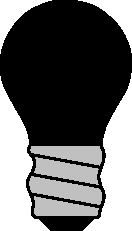
\includegraphics[height=.6cm]{images/pictures/bulb_off.pdf}}}$} % Detector off (waiting)
\newcommand{\DetectorOn}{$\vcenter{\hbox{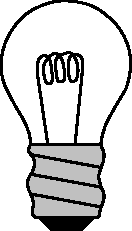
\includegraphics[height=.6cm]{images/pictures/bulb_on.pdf}}}$} % Detector on (activated)
\newcommand{\Atom}{$\vcenter{\hbox{
\includegraphics[height=.4cm]{images/pictures/atom.pdf}}}$} % Atom
\newcommand{\Photon}{$\vcenter{\hbox{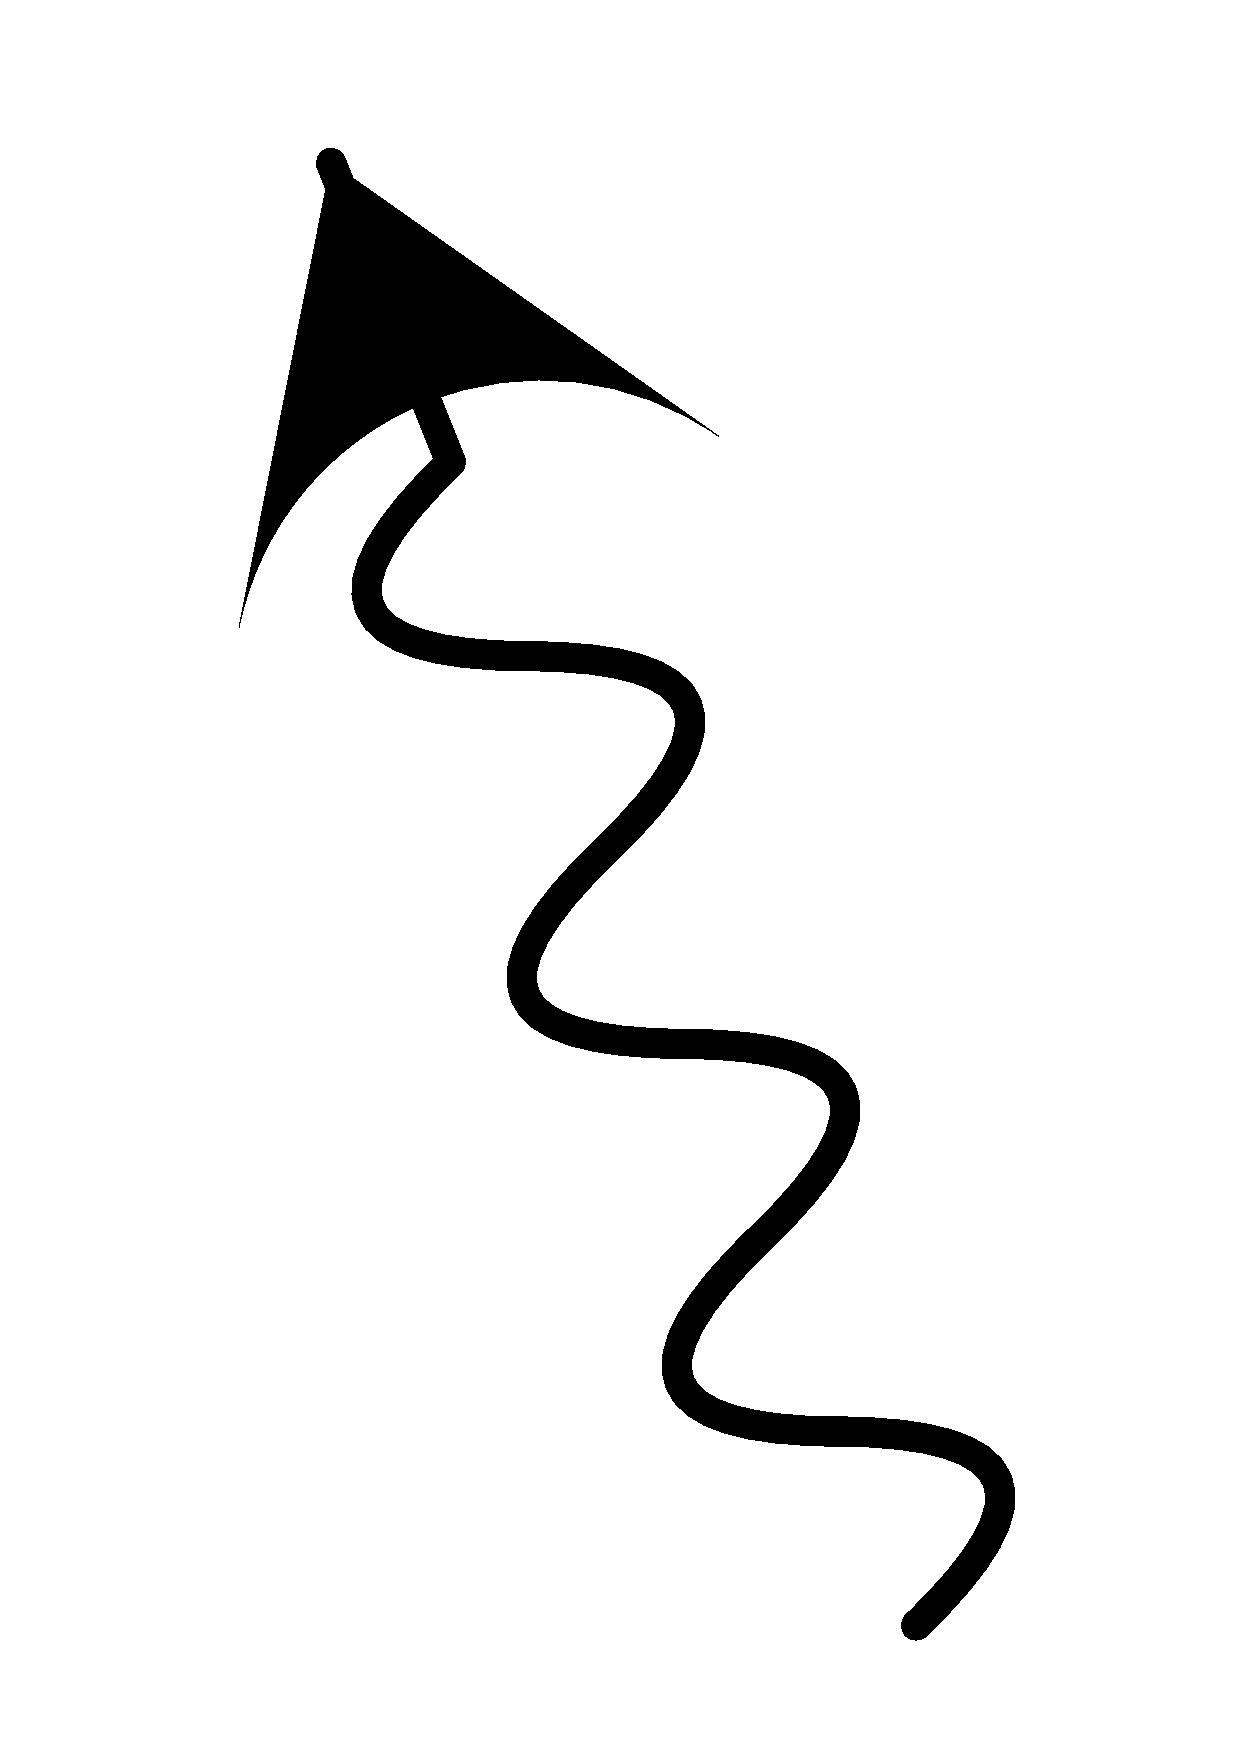
\includegraphics[height=.6cm,angle=-90,origin=c]{images/diagrams/Photon.pdf}}}$} % Photon
\newcommand{\ObserverOff}{$\vcenter{\hbox{\huge\textit?}}$} % Observer off (waiting)
\newcommand{\ObserverOn}{$\vcenter{\hbox{\huge\textit!}}$} % Observer on (having observed the expected result)
\newcommand{\Superposition}{$\vcenter{\hbox{\huge+}}$} % Quantum superposition

\frontmatter

\thispagestyle{empty}

\null
\vfill
\begin{center}
{\Huge \textbf{Quantum\\Ethics}}
\vskip 1.2cm
A Spinozist Interpretation \\
of Quantum Field Theory
\vskip 2cm
{\large Sébastien Fauvel}
\end{center}
\vfill
\null

\newpage

\null
\vfill
\noindent{\small Cover image: Hubble telescope image of the Carina Nebula, 2007.\\
Photograph: NASA, ESA, N. Smith (University of California, Berkeley), and The Hubble Heritage Team (STScI/AURA).}

\cleardoublepage
\section*{Acknowledgements}

First and foremost, I would like to thank my wife Angela for having let me enjoy her wisdom and love radiating being for all these years. She made me discover Spinoza's philosophy and this publication would never have been possible without the help of her brilliant intelligence, of her constructive criticism, of all her love and support. Thank you!

I would also like to thank my colleague Markus Matteucci for initiating me into the art of book publishing, my fellow students Christian Hagendorf and Tristan Machado for some fruitful discussions that did much for my understanding of Physics, my teachers Christian Swit and Stéphane Gentil who introduced me to the joys of Philosophy and Mathematics, my uncle Bertrand Liaudet and my regretted ``godfather'' Frédéric Poupaud for having made me discover the world of Algorithmic and Informatics at a far too early age. They all did very much for my personal evolution.

\cleardoublepage
\section*{Preface}

This book has been written with the main concern of providing the scientific community with a mean of building a bridge between physicists and philosophers in the field of Quantum Physics. It defines a common language to describe the realm of our experience of the world and I truly hope that this new language will find a large audience in both communities. For physicists, it stresses the importance of developing a well-defined mathematical formalism for Quantum Field Theory, since this is the necessary condition for philosophers to identify the underlying ontology, which builds the base of every philosophical discourse on the implications of Quantum Physics. The development of a coherent, convincing discourse by philosophers builds in turn the ground on which every conceptually and technically correct vulgarization effort can foot, and contributes thereby to broaden the popularity and acceptance of Quantum Physics through the whole society and especially among prospective students. Philosophers, on the other hand, gain a mean of confronting their ideas with the latest insights into fundamental physics, of expressing these ideas in terms of naturalistically grounded metaphysics and of articulating speculative thoughts in the uncertainty zones remaining within the physical theory itself or inherent to it.

The careful reader already familiar with Quantum Physics will find here the very first mathematically well-defined formulation of Quantum Field Theory coming along with an intellectually satisfactory interpretation, perfectly capable of explaining all known quantum phenomena, and I am very pleased to present it to your curiosity today! However, although you will find, in the first edition of this book, all the main ideas I wanted to develop here, there still are a few areas which I couldn't yet find the time to develop to the extend they would have deserved. For instance, I do consider the formulation of Quantum Field Theory presented in this book, which is essentially a lattice regularization, as an acceptable fundamental theory, although it obviously lacks to respect the heuristical principles of Gauge and Poincaré invariance on which any textbook introduction to Quantum Field Theory relies. I included a few calculation examples in order to demonstrate that, at usual energy and distance scales, the resulting physics is the same as expected, but it would have been useful, to convince the skeptical reader, to add a classical renormalization example, a treatment of the weak and strong interactions as well as of the Higgs mechanism and of some gravitational model. The philosophical aspects of this book might have deserved a more extensive treatment, too. I have given a few basic examples to show how the physical theory can be used as a reference language in order to express philosophical questions, but I would have to add more various examples to give an adequate idea of the potential of this method.

I am preparing a second, augmented edition of this work so that the ideas presented here become more explicit and accessible to a broader public. For the time being, I wish you a fruitful and enjoyable reading as well as long hours of delightful meditation!

\begin{flushright}
\begin{tabular}{l}
January, 2013\\
Sébastien Fauvel
\end{tabular}
\end{flushright}

\cleardoublepage
\tableofcontents

\mainmatter

\chapter*{History of this book}

\renewcommand{\epigraphwidth}{8.3cm}
\epigraph{For one of the most stringent tests of any physical theory is the prediction of its own creation process.}{Sébastien Fauvel,\\\textit{Quantum Ethics}~\cite{Fauvel2013}}

How would Quantum Field Theory look like if we stopped for a while developing it further as if it were the draft of a yet-to-be-discovered Theory of Everything, and just started to reformulate the Standard Model as a mathematically and conceptually coherent physical theory? And what would such a theory tell us about the world and about ourselves, which remains hidden in the ill-defined formulations we've grown up with through the last decades? As I started back in 2010 to reflect on these questions, I didn't have yet a clear vision of what this work would lead me to. I just had the feeling that these very basic questions hadn't been interesting anyone any more for a far too long time, and that we should actually have the means by now, with our understanding of Renormalization, of writing down a well-defined Quantum Field Theory, reasonably accounting for all known experimental data (excepted General Relativity phenomena), which means essentially that it has to be compatible with the Standard Model at known energy scales. I was quite confident that I could find a physically sound regularization of the Standard Model, which I simply wouldn't consider as an approximation, but take as the exact theory itself, the Standard Model being an ill-defined idealization of it. The models used in computer simulations of lattice Quantum Chromodynamics, for instance, would show me the way. Of course, I knew that I wouldn't be able to derive the theory from the usual first principles any more, but given that all the attempts of axiomatic Quantum Field Theory to construct well-defined interacting fields upon these first principles had failed miserably, I thought that maybe they could be misleading in the end. Anyhow, I had never been very fond of the heuristical construction of Quantum Field Theory based on Gauge and Poincaré invariance. Developing the whole mathematical apparatus of Representation Theory to simply derive the expression of spin 1 and spin 1/2 spinors as irreducible unitary representations of the Poincaré group had always seemed far too expensive to me, and Gauge transformations mixing particle fields far too artificial to make up a fundamental symmetry of Nature.

\chapter*{Introduction}

\section*{Interpreting Quantum Field Theory}

The birth of Quantum Physics in the 1920s has been marked by a long period of intense controversies about its interpretation, which has been recently reviewed by Juan Miguel Marin in his paper \textit{‘Mysticism’ in quantum mechanics: the forgotten controversy}~\cite{Marin2009}. The Copenhagen interpretation which emerged from these debates is dominating the scene since the 1950s-1960s, certainly not because it is intrinsically better than others, but because it seems to challenge the materialist world view of classical, `everyday' physics as little as possible. Since the 1970s, however, numerous alternative interpretations have been proposed and further developed: Pilot-Wave Theory, Dynamical Collapse Theories, Many-Worlds interpretation, Many-Minds interpretation, Decoherent Histories... All these attempts to give Quantum Physics a sound interpretation are facing the problem that the mathematical theory itself, in the form of the Standard Model of Quantum Field Theory (or of slight variants regarding the existence of the Higgs field, of neutrino masses...), is still ill-defined, and that it is therefore impossible to assign a physical or metaphysical meaning to the fundamental mathematical entities of the theory, i.e. to define an ontology. Of course, it is possible to choose a specific, mathematically well-defined regularization of the theory for this purpose, but since renormalization methods are leading, in the singular limit of the original theory, to the same results for different regularization schemes, we don't know which regularization is the right one, and as a consequence we don't know either which are the fundamental mathematical entities to be interpreted. Quite surprisingly, however, it seems that this issue has never been seriously accounted for yet. Existing interpretations of Quantum Physics are either restricted to non-relativistic Quantum Mechanics, which is no fundamental theory, or are formulated so vaguely that they are hardly more than the mere idea of an interpretation, which has made many physicists doubt that such an interpretation is possible at all. This book will have reached his goal if it convinces the reader of the contrary and helps interpretation issues recovering again their place at the heart of the research on Quantum Field Theory. For this purpose, I shall take as an example a lattice regularization scheme, formulate in this well-defined framework a rather conservative interpretation inspired by Spinoza's philosophy and show that classical philosophical questions can be formulated as simple physical hypotheses in the frame of the resulting naturalistic metaphysics.

\section*{Philosophical motivation}

Most philosophers have ascribed a central role to the ethics in their work, as the answer to the question ``How should I live?'' requires a preliminary reflection about all the fields of our existence, from metaphysics via physics, psychology and morals up to politics. Up to the emergence of Quantum Field Theory in the late 1920s, philosophers have always been able to integrate the knowledge gathered in the field of physics into their world view: In 17th-century Europe, for instance, the Dutch philosopher Baruch Spinoza worked out in his \textit{Ethics}~\cite{Spinoza1677} the deterministic materialism of classical mechanics and based his philosophy on the idea that everything in Nature happens according to the divine necessity, both at the material and at the spiritual level. In fact, from the Antics up to the Age of Enlightenment, physicists used to consider themselves primarily as Nature philosophers. In the modern ages, however, the scientific community began to split under the influence of industrial work organization into small groups of specialists lacking interdisciplinary skills. Nowadays, mainstream physicists even consider philosophical interpretations of Physics as non-scientific and pointless. Needless to say, such a lack of intellectual rigor has had serious consequences for the conceptual and formal quality of physical theories. In the case of Quantum Field Theory, this attitude has resulted in the fact that, for the last eighty years, no consensus could be reached on its two major issues, known as the \textit{measurement problem} and the \textit{main issue}. The latter is a formal issue consisting in conceiving a mathematically well-defined quantum field theory formally compatible to Special Relativity\footnotemark[1], which would be highly desirable but is thought to be technically impossible, although this hasn't been proved definitely yet. The former is an interpretation issue concerning the relation between ``mind'', i.e. the primitive form of our experience of the world, and ``body'', i.e. the physical world described in terms of quantum fields. There have been numerous propositions for this interpretation, from the very beginning of Quantum Field Theory in the 1920s and 1930s until now, but as long as the mathematical formalism of the theory is ill-defined, these interpretations cannot be formulated precisely either. Strictly speaking, however, the whole theory doesn't make any sense if this interpretation issue doesn't become precisely answered. In order to give a sound philosophical interpretation of Quantum Field Theory, it is therefore necessary in the first place to put the mathematical formalism on a well-defined basis. The theory cannot be formally compatible with Special Relativity if the main issue really cannot be solved; Relativity Theory should then emerge as an approximation at usual energy and distance scales. In this book, I shall propose an answer to both issues, describe very precisely the form of the relation between mind and body according to Quantum Physics and thus lay the foundations of an ethic taking into account the world view sustained by Quantum Field Theory.

\footnotetext[1]{Precisely, one requires that the classical Lagrangian used in the heuristical construction of the theory be Poincaré invariant and describes local (contact) interactions of point particles in the Minkowski space-time.}

\section*{Abstract}

In the formulation of Quantum Field Theory proposed in this book, Nature presents the two aspects of a physical and of a mental world in mutual interaction. The mental world can be adequately experienced by the collectivity of all sentient beings: A state of the mental world is given by a set of a various number of individual minds with definite conscious thoughts. Though we are experiencing this mental world directly, we only experience it partially under the aspect of a single individual mind (which we're used to call ``our'' mind), and must communicate with others in order to get closer to an adequate representation of the mental world as a whole. Communication happens in the physical world, which is an aspect of Nature that we don't experience directly but only through its influence on our subjective mental experience. This physical world, best described in terms of quantum fields, is by nature holistic and doesn't involve precise boundaries of individual bodies as they may exist for individual minds. A state of this physical world is given by a quantum superposition of so-called localized states, which are given by the number of elementary particles of each kind present at each point of space. Each physical state can be uniquely decomposed into a sum of components corresponding to each possible mental state, and this decomposition defines a probability law on the set of all possible mental states. The joined temporal evolution of both aspects of Nature is a tree-steps process repeated indefinitely: First, the initial state of the physical world undergoes a deterministic, Hamiltonian evolution of a given, ``elementary'' duration. Then, the final physical state defines a probability law according to which a mental state is being selected and becomes collectively experienced. Finally, the component of the physical state corresponding to the selected mind state becomes the initial state of the next evolution process. In this world view, the mystery of consciousness consists in the fact that there is, to some extent, an adequation between the conscious thoughts of individual minds and some physical processes happening in the corresponding physical states, e.g. the biological processes of consciousness within a human brain.

\section*{Overview}

This book begins in chapter \ref{Quantum fields} with the formulation of a mathematically well-defined frame for any theory of mutually interacting quantum fields of point particles. Well-definedness is achieved by making sure that the Hamilton space of the quantum states is finite dimensional, so that the Hamiltonian evolution is trivially well-defined for any interaction Hamiltonian. The ``ingredients'' of this mathematical frame are already well-known in Quantum Field Theory: Space is supposed to have the structure of a finite three dimensional lattice, the definition of the kinetic energy Hamiltonian making use of the SLAC derivative, and the occupation number of single modes of the particle fields is supposed to be bounded for bosons as well as for fermions.

The Hamiltonian evolution of quantum fields is then defined very classically for an arbitrary interaction Hamiltonian in chapter \ref{Hamiltonian evolution}, where general results of scattering theory are being derived.

A general model for the mental world is defined in chapter \ref{Mental states} and the joint stochastic evolution of the physical and mental worlds in chapter \ref{Stochastic evolution}. The basic idea of this model -- that ``mind causes collapse'' -- isn't quite new, as it has first been formulated by John von Neumann~\cite{Neumann1932} and was once known as the `standard interpretation' of Quantum Mechanics. As far as I know, however, it is the first time with this book that a precise interpretation of a mathematically well-defined Quantum Field Theory has ever been given. This provides thus the first sound basis for a discussion of the philosophical implications of the theory, which is the main goal of this book.

The metaphysics of the theory are been sketched in chapter \ref{Metaphysics} and its interpretation discussed at length in chapter \ref{Interpretation}. A few classical philosophical questions are then addressed on this background in chapter \ref{Philosophical issues}.

The interaction Hamiltonian of Quantum  Electrodynamics is then defined in chapter \ref{Quantum Electrodynamics} and, as an example, the semi-classical cross-section of Coulomb scattering is calculated to the leading order in chapter \ref{Coulomb scattering}.

Finally, some usual mathematical functions, notations and operators are being defined in the appendix.

\part{Physical world}

\chapter{Quantum fields}
\label{Quantum fields}

\renewcommand{\epigraphwidth}{7cm}
\epigraph{The first simplification to be considered involves the very existence of the theory.}{John Collins,\\\textit{Renormalization}~\cite{Collins1984}}

The aim of this chapter is to develop a well-defined, divergence-free mathematical formalism for the Standard Model of particle physics. To achieve this, we suppose that elementary particles are bounded to a finite lattice, also a finite set of world lines in the flat space-time (so that the particle field only has a finite number of modes), and that there is a maximum occupation number for any single mode of the field, for bosons as well as for fermions. This makes the Hilbert space of the states of the universe finite dimensional, so that the theory is trivially well-defined. We will develop here a general formalism, valid for any set of elementary particles and for any form of the interaction Hamiltonian, and define the notations used in the rest of this book.

\section{Space}

\paragraphtitle{Definition} Space is a finite set of points of the form $\FL$, where the physical constant $\N$ is a positive integer.

\paragraphtitle{Remarks} This constant is supposed to be a ``huge'' integer ($\gtrsim~10^{46}$) which hasn't been measured experimentally yet. The finiteness of space is one of the conditions of the finite dimensionality of the Hilbert space of the physical states, which will be defined in section \ref{Many particles states}. This is in turn a necessary condition of the well-definedness of the evolution equation \ref{Schrödinger equation} for an arbitrary Hamiltonian operator. It is therefore a theoretical necessity, which I shall assume although this fact hasn't been proved experimentally yet.

\paragraphtitle{Commentaries} No notion of distance emerges from this definition of space. Indeed, according to the ideas developed in Einstein's vulgarization work \textit{Relativity: The Special and General Theory}~\cite{Einstein1916}, we consider that distance and duration are actually no fundamental notions but have to be defined on an empirical basis. Distance and duration are measured using physical apparatus like rods or clocks, and their theoretical definition must rely on a theoretical modeling of these apparatus and of the observer making use of them. These concepts will emerge from the evolution equation \ref{Schrödinger equation} and from the expression of the Hamiltonian operator defined in sections \ref{Kinetic energy Hamiltonian} and \ref{QED interaction Hamiltonian}. According to this expression, we will see that space has a toroidal structure, i.e. that opposite points on the boundary of the lattice $\FL$ are actually nearest neighbors. This boundary is also a mere artifact, like the boundary of a world map, and doesn't represent in any way the ``frontier of the universe''. The physical constant $\a$ in the expression of the interaction Hamiltonian plays the role of the lattice step, i.e. of the distance between nearest neighbors. It is supposed to be very small ($\lesssim~10^{-20}~\mathrm m$) and hasn't yet been measured experimentally either.

\paragraphtitle{Complements} We could equivalently postulate that, in the Minkowski space-time $(\ST,\stt g)$, defined by:
\begin{eqnarray*}
\ST & \eqdef & \IR^4 \\
\stt g & \eqdef & diag(1,-1,-1,-1) \\
\stv x \stsp \stv y & \eqdef & \sttll g \mu \nu \stvh x \mu \stvh y \nu
\end{eqnarray*}
elementary particles cannot occupy an arbitrary point of space but are bounded to a finite set of $(1+2 \N)^3$ world lines $\wl \n$ forming in some reference frame a finite lattice of step $\a$:
\begin{eqnarray*}
\wlt \n \tau & \eqdef & \matrix{\c \tau \\ \a \n} \\
\n & \in & \FL
\end{eqnarray*}

In a reference frame moving with a velocity $\sv v$ relative to the lattice, the space-time coordinates of these world lines would be given (up to a translation of the origin) by:
\begin{eqnarray*}
\wltp \n t & = & \matrix{\c t \\ \a  \n_\perp + \gamma^{-1} \a  \n_\parallel - \sv v t} \\
\gamma & \eqdef & \frac 1 {\sqrt{1 - (v / \c)^2}}
\end{eqnarray*}
where we use the notations $\n_\parallel \eqdef ( \n \ssp \sv v ) \sv v / v^2$ and $\n_\perp \eqdef \n - \n_\parallel$.

The lattice reference frame itself as well as the physical constants $\N$ and $\a$ are free parameters of the theory. As a working hypothesis, we will assume that the lattice reference frame corresponds to a rest frame of the cosmic microwave background radiation. The relative velocity $\sv v$ of the sun relative to the lattice would then verify~\cite{Kogut1993}:
\begin{equation*}
v \approx 3.7~10^5\ \mathrm m / \mathrm s
\end{equation*}
We will also assume that the lattice step is of the order of the Plank length:
\begin{equation*}
\a \sim \sqrt{4\pi\G \h/\c^3}\approx1.4~10^{-34}\ \mathrm m
\end{equation*}
and that the lattice size is of the order of the Hubble length~\cite{Freedman2001}:
\begin{eqnarray*}
(1+2 \N) \a & \sim & \RH\approx1.3\ 10^{26}\ \mathrm m\\
\N & \sim & 4.6~10^{59}
\end{eqnarray*}
Incidentally, with this values, the cosmological constant of the $\Lambda$-Cold Dark Matter model of Big-Bang cosmology coincides numerically (with a relative error of only 8\%) with~\cite{Komatsu2010}:
\begin{equation*}
\rho_{vac} \sim 2 \N \frac{\h \c}{\a} \left( ( 1 + 2 \N ) \a \right)^{-3} \approx 5.6~10^{-10}\ \mathrm J / \mathrm m^3
\end{equation*}
Deriving such a relation, however, isn't the goal of this book.

\section{One particle states}

\paragraphtitle{Particle types} We don't make in this chapter any assumption about the existing particle types, e.g. electrons, positrons and photons. We are noting them $\pt$ in a generic way. The corresponding spin states $\sp$ depend implicitly, in the notations, on the particle type. The spin state influences the way a particle interacts with other particle fields; this effect is described quantitatively in the expression of the spinor operators in appendix \ref{Photon spinors} and \ref{Dirac spinors}.

\paragraphtitle{Definition} The (hypothetical) physical state $\ket{\Psi}$ in which the universe only contains a single particle, of type $\pt$, at point $\n$ and in the spin state $\sp$, is written:
\begin{equation*}
\ket{\Psi} = \ketX 1 \pt \n \sp
\end{equation*}

We postulate that a one particle state is given by any linear combination of the form:
\begin{equation*}
\ket{\Psi} = \sum_{\pt,\n,\sp} \Psi(\bX 1 \pt \n \sp) \ketX 1 \pt \n \sp
\end{equation*}
with arbitrary complex coefficients $\Psi(\bX 1 \pt \n \sp)$. The set of all these vectors, taken as an orthonormal basis, forms a finite dimensional Hilbert space written $\Hn 1$ and given by:
\begin{equation*}
\Hn 1 \eqdef \bigoplus^\perp_{\pt,\n,\sp} \IC \ketX 1 \pt \n \sp
\end{equation*}

\paragraphtitle{Momentum representation} We postulate that the momentum $\p$ of a particle in the lattice reference frame can only take values of the form:
\begin{eqnarray*}
\p & = & \frac \h \a \q\\
\q & \in & \FLD
\end{eqnarray*}
and that the (hypothetical) physical state in which the universe only contains a single particle, of type $\pt$, in the spin state $\sp$ with the momentum $\h\q / \a$ in the lattice reference frame, is given by:
\begin{equation*}
\ketQ 1 \pt \q \sp \eqdef (1+2 \N)^{-3/2} \sum_{\n} \exp{\i 2 \pi \n \ssp \q} \ketX 1 \pt \n \sp
\end{equation*}

These vectors form an orthonormal basis of the Hilbert space $\Hn 1$ and we will use the notation:
\begin{equation*}
\ket\Psi = \sum_{\pt,\q,\sp} \FT\Psi(\bQ 1 \pt \q \sp) \ketQ 1 \pt \q \sp
\end{equation*}

\paragraphtitle{Notation} In order to simplify the notations, when defining and using periodical functions on all $\q \in \IR^3$, we will define $\eqp \q \in \left]-\frac 1 2,\frac 1 2\right]^3$ by the equivalence relation $\eqp \q - \q \in \IZ^3$. We have then in particular $\eqp \q = \q$ for all $\q \in \FLD$ and $\eqp \q \in \FLD$ for all $\q \in \ILD$.

\section{Position and momentum operators}

\paragraphtitle{Definition} In the lattice reference frame, we define on $\Hn 1$ the position and momentum operators by:
\begin{eqnarray*}
\Rop \ketX 1 \pt \n \sp & \eqdef & \a \n \ketX 1 \pt \n \sp \\
\Pop \ketQ 1 \pt \q \sp & \eqdef & \frac \h \a \q \ketQ 1 \pt \q \sp
\end{eqnarray*}

\paragraphtitle{Remark} This definition of the momentum operator follows the same principle as the SLAC derivative~\cite{Rabin1981}, but can be expressed as a proper eigenvalue equation, since momentum eigenstates are well-defined on a finite lattice.

\paragraphtitle{Complements} In another reference frame, moving with a velocity $\sv v$ relative to the lattice, these operators are given (up to a translation of the origin) by:
\begin{eqnarray*}
\Rop \ketX 1 \pt \n \sp & \eqdef & \left( \a \n_\perp + \gamma^{-1} \a  \n_\parallel - \sv v t \right) \ketX 1 \pt \n \sp \\
\Pop \ketQ 1 \pt \q \sp & \eqdef & \left( \frac \h \a \q_\perp + \gamma \frac \h \a \q_\parallel - \gamma \frac {\Ek \pt \q} {\c^2} \sv v \right) \ketQ 1 \pt \q \sp
\end{eqnarray*}
where $\Ek \pt \q$ is the kinetic energy of the particle in the lattice reference frame, defined as a function of its (bare) rest mass $\mp \pt$ by:
\begin{equation*}
\Ek \pt \q \eqdef \sqrt{\left( \mp \pt \c^2 \right)^2 + \left( \frac{\h \c}{\a} \eqp \q \right)^2}
\end{equation*}
Similarly, we define the relativistic factors $\bk \pt \q$ and $\gk \pt \q$, with the help of the reduced mass $\mpr \pt \eqdef \mp \pt \a \c / \h$, by:
\begin{equation*}
\bk \pt \q \eqdef \frac{\eqp \q}{\sqrt{\mpr \pt^2 + \eqp \q^2}}
\end{equation*}
\begin{equation*}
\gk \pt \q \eqdef \sqrt{1 + \left( \frac{\eqp \q}{\mpr \pt} \right)^2}
\end{equation*}
and the velocity by $\vk \pt \q \eqdef \bk \pt \q \c$.

\section{Wave function}

\paragraphtitle{Remark} We can associate following wave function components to each one particle state:
\begin{equation*}
\wf \Psi \pt \sp {\sv x} \eqdef (1+2 \N)^{-3/2} \sum_{\q} \FT\Psi(\bQ 1 \pt \q \sp) \exp{\i 2 \pi \frac{\sv x \ssp \q}{\a}}
\end{equation*}
Eigenstates of the momentum operator are thus associated with plane waves on $\IR^3$. Equivalently, we can write:
\begin{eqnarray*}
\wf \Psi \pt \sp {\sv x} & = & \sum_{\n} \Psi(\bX 1 \pt \n \sp) \deltaX{\sv x - \a \n} \\
\deltaX{\sv x} & \eqdef & (1+2 \N)^{-3} \prod_i \frac{\sin{\pi \svc x i / \a}}{\sin{\pi \svc x i / (1+2 \N)\a}}
\end{eqnarray*}
We define thus an isomorphism between a finite set, indexed on $( \pt,\sp )$, of complementary subspaces of $\Hn 1$, and a finite dimensional subspace of $\mathrm C^\infty\left(\IR^3,\IC\right)$ containing functions of period $(1+2\N)\a$ along each coordinate.

\paragraphtitle{Complements} In that space, the (image of the) momentum operator acts according to:
\begin{equation*}
\Pop \wf \Psi \pt \sp {\sv x} = \frac{\h}{\i 2 \pi} \sv \nabla \wf \Psi \pt \sp {\sv x}
\end{equation*}
The dynamic of the free fields on the lattice is also identical to the usual dynamic of the free fields on the continuum in the box $\left]-(\N+\frac 1 2)\a,(\N+\frac 1 2)\a\right[^3$ with periodical boundary conditions.

\section{Many particles states}
\label{Many particles states}

The physical state $\ket{\Psi}$ in which each point $\n$ is being occupied by $\bX N \pt \n \sp$ particles of each type $\pt$ in each spin state $\sp$ is written:
\begin{equation*}
\ket{\Psi} = \ketFX N \pt \n \sp
\end{equation*}
and is called a ``localized state''. We postulate that a many particles state is given by any linear combination of the form:
\begin{eqnarray*}
\ket{\Psi} & = & \sum_{\bFX N \pt \n \sp} \Psi \left(\bFX N \pt \n \sp \right) \ketFX N \pt \n \sp \\
\bX N \pt \n \sp & \in & \IntRange{0}{\M \pt}
\end{eqnarray*}
where the (finite) integer $\M \pt$ is the maximum occupation number of the field $\pt$.

The set of all these vectors, taken as an orthonormal basis, forms a finite dimensional Hilbert space given by:
\begin{equation*}
\H \eqdef \bigoplus^\perp_{\bFX N \pt \n \sp} \IC \ketFX N \pt \n \sp
\end{equation*}
and the basis of the localized states is called ``position basis''.

\paragraphtitle{Remark} For fermions, we have experimentally $\M \pt = 1$. For bosons, no upper limit of the occupation number is experimentally known; a lower limit of about $\M \photon \gtrsim 10^{21}$ for photons has been reached experimentally by high intensity lasers.

\section{Creation and annihilation operators}

\paragraphtitle{Definition} The annihilation operators are given by:
\begin{equation*}
\aop \pt \n \sp \ket{\bFX N \pt \n \sp} \eqdef \begin{cases}
\ket{\bFX N \pt \n \sp - \bX 1 \pt \n \sp} & \text{if $\bX N \pt \n \sp > 0$} \\
0 & \text{otherwise}
\end{cases}
\end{equation*}
and the creation operators by:
\begin{equation*}
\cop \pt \n \sp \ket{\bFX N \pt \n \sp} \eqdef \begin{cases}
\ket{\bFX N \pt \n \sp + \bX 1 \pt \n \sp} & \text{if $\bX N \pt \n \sp < \M \pt$} \\
0 & \text{otherwise}
\end{cases}
\end{equation*}

The (hypothetical) state of the universe in which no particles are present is written:
\begin{equation*}
\ket \Psi = \ket{\vac} \eqdef \ket{\bFX 0 \pt \n \sp}
\end{equation*}

\paragraphtitle{Remark} The annihilation (resp. creation) operators form a (finite) set of generators of a commutative algebra $\aAlg$ (resp. $\cAlg$). Any state of the universe can be obtained by applying creation operators on the vacuum according to:
\begin{eqnarray*}
\ket{\Psi} & = & \dop{\Psi} \ket{\vac} \\
\dop{\Psi} & \eqdef & \sum_{\bFX N \pt \n \sp} \Psi \left(\bFX N \pt \n \sp \right) \prod_{\pt,\n,\sp} \left( \cop \pt \n \sp \right)^{\bX N \pt \n \sp}
\end{eqnarray*}
associating thus an operator $\dop{\Psi} \in \cAlg$ to each vector $\ket{\Psi} \in \H$ canonically.

\paragraphtitle{Commentaries} We are defining here at purpose very basic creation and annihilation operators. The normalization factor relevant for boson fields and the antisymmetry factor relevant for fermion fields are included explicitly in the interaction Hamiltonian, e.g. in the photon spinor operators defined in appendix \ref{Photon spinors} and in the Dirac spinor operators defined in appendix \ref{Dirac spinors}.

\section{Plane wave field modes}

\paragraphtitle{Definition} Creation and annihilation operators can also be defined for the plane wave modes of the field by:
\begin{eqnarray*}
\aop \pt \q \sp & \eqdef & (1+2 \N)^{-3/2} \sum_{\n} \exp{-\i 2 \pi \n \ssp \q} \aop \pt \n \sp \\
\cop \pt \q \sp & \eqdef & (1+2 \N)^{-3/2} \sum_{\n} \exp{\i 2 \pi \n \ssp \q} \cop \pt \n \sp
\end{eqnarray*}
Note that this definition can be extended to all $\q \in \IR^3$. The plane wave states of the field are then defined by:
\begin{equation*}
\ket{\bFQ N \pt \q \sp} \eqdef \prod_{\pt,\q,\sp} \left( \cop \pt \q \sp \right)^{\bQ N \pt \q \sp} \ket{\vac}
\end{equation*}
These vectors form an orthonormal basis of the Hilbert space $\H$ called the ``momentum basis'' and we will use the notation:
\begin{equation*}
\ket\Psi = \sum_{\bFQ N \pt \q \sp} \FT\Psi \left( \bFQ N \pt \q \sp \right) \ket{\bFQ N \pt \q \sp}
\end{equation*}

\paragraphtitle{Remark} The decomposition of the plane wave state $\ket{\bFQ {N'} \pt \q \sp}$ on the position basis is given by:
\begin{eqnarray*}
\braket{\bFX N \pt \n \sp}{\bFQ {N'} \pt \q \sp} & = & \left[ \prod_{\pt, \sp} \delta\left( {N'}^\pt_\sp - N^\pt_\sp \right) \right] \psi \left( ( \q^{\pt, \sp}_j ), ( \n^{\pt, \sp}_j ) \right) \\
\psi \left( ( \q^{\pt, \sp}_j ), ( \n^{\pt, \sp}_j ) \right) & \eqdef & \prod_{\substack{\pt, \sp \\ N^\pt_\sp \neq 0}} \frac{(1+2 \N)^{-3 N^\pt_\sp / 2} }{\prod_{\n} \bX N \pt \n \sp !} \sum_{\sigma \in \mathfrak{S}_{N^\pt_\sp}} \prod_{j = 1}^{N^\pt_\sp} \exp{\i 2 \pi \n^{\pt, \sp}_{\sigma_j} \ssp \q^{\pt, \sp}_j}
\end{eqnarray*}
where we use the notations ${N'}^\pt_\sp \eqdef \sum_{\q} \bQ {N'} \pt \q \sp$ and $N^\pt_\sp \eqdef \sum_{\n} \bX N \pt \n \sp$, where $\mathfrak{S}_{N^\pt_\sp}$ denotes the symmetric group of order $N^\pt_\sp$ and where we have chosen for each mode $( \pt, \sp )$ of the field the families $( \n^{\pt, \sp}_j )$ and $( \q^{\pt, \sp}_j )$ such as:
\begin{eqnarray*}
\ket{\bFX N \pt \n \sp} & = & \prod_{\pt, \sp, j} \cop \pt {\n^{\pt, \sp}_j} \sp \ket{\vac} \\
\ket{\bFQ {N'} \pt \q \sp} & = & \prod_{\pt, \sp, j} \cop \pt {\q^{\pt, \sp}_j} \sp \ket{\vac}
\end{eqnarray*}
In the definition of $\psi \left( ( \q^{\pt, \sp}_j ), ( \n^{\pt, \sp}_j ) \right)$, we used for convenience the symbols $\bX N \pt \n \sp$ and $N^\pt_\sp$, which can be defined as a function of $( \n^{\pt, \sp}_j )$ with $\bX N \pt \n \sp \eqdef \left|  \{ j | \n^{\pt, \sp}_j = \n \} \right|$.

\section{Particle number operators}

\paragraphtitle{Definition} The particle number operators are defined by:
\begin{eqnarray*}
\Nop \pt \n \sp \ket{\bFX N \pt \n \sp} & \eqdef & \bX N \pt \n \sp \ket{\bFX N \pt \n \sp} \\
\Nop \pt \q \sp \ket{\bFQ N \pt \q \sp} & \eqdef & \bQ N \pt \q \sp \ket{\bFQ N \pt \q \sp}
\end{eqnarray*}
The total particle number operator is defined as the (finite) sum:
\begin{equation*}
\op N \eqdef \sum_{\pt,\n,\sp} \Nop \pt \n \sp = \sum_{\pt,\q,\sp} \Nop \pt \q \sp
\end{equation*}
Its eigenspace for the eigenvalue $N$ is written $\Hn N$ and its elements are called ``$N$ particle states'' of the field. The Hilbert space can be decomposed as a (finite) sum of the form:
\begin{equation*}
\H = \bigoplus_{N}^\perp \Hn N
\end{equation*}
The maximum number of particles in a $N$ particle state is given by $N = (1+2 \N)^3 \sum_{\pt,\sp} \M \pt$.

\chapter{Hamiltonian evolution}
\label{Hamiltonian evolution}

\section{Schrödinger equation}
\label{Schrödinger equation}

We postulate that the state of the quantum field evolves according to an equation of the form:
\begin{equation*}
\ddt \ket\Psi = -\i 2 \pi \frac 1 \h \Hop \ket\Psi
\end{equation*}
called ``Schrödinger equation'' where $\Hop$ is the (time independent) Hamiltonian operator of the field. This operator is supposed to be hermitian and is therefore diagonalizable (with real eigenvalues) on the finite dimensional Hilbert space $\H$. The equation can also be integrated as:
\begin{eqnarray*}
\ket{\Psi(t)} & = & \Uop t {t_0} \ket{\Psi(t_0)} \\
\Uop t {t_0} & \eqdef & \exp{- \i 2 \pi \frac{t - t_0} \h \Hop}
\end{eqnarray*}

\section{Kinetic energy Hamiltonian}
\label{Kinetic energy Hamiltonian}

The Hamiltonian operator of the field can be separated into a kinetic energy Hamiltonian depending only on the momentum of the particles and an interaction term as follows:
\begin{equation*}
\Hop = \Hop_0 + \Hop'
\end{equation*}
In the lattice reference frame, the kinetic energy Hamiltonian is given by:
\begin{equation*}
\Hop_0 \eqdef \sum_{\pt,\q,\sp} \Ek \pt \q \Nop \pt \q \sp
\end{equation*}

In another reference frame, moving with a velocity $\sv v$ relative to the lattice, this operator is given by:
\begin{equation*}
\Hop_0 \eqdef \sum_{\pt,\q,\sp} \gamma \left\{ \Ek \pt \q - \frac \h \a \q \ssp \sv v \right\} \Nop \pt \q \sp
\end{equation*}

\section{Interaction picture}

The kinetic energy Hamiltonian can be integrated as:
\begin{equation*}
\UopK t {t_0} \eqdef \exp{- \i 2 \pi \frac{t - t_0} \h \Hop_0}
\end{equation*}

The state of the quantum field in the interaction picture is defined in such a way that it would be a time constant if the interaction term $\Hop'$ vanishes:
\begin{equation*}
\ket{\Psi_\I} \eqdef \UopK 0 t \ket{\Psi}
\end{equation*}

The Hamiltonian operator in the interaction picture is defined is such a way that the state of the quantum field in the interaction picture obeys following Schrödinger-like equation, where the Hamiltonian is time-dependent:
\begin{eqnarray*}
\ddt \ket{\Psi_\I} & = & -\i 2 \pi \frac 1 \h \Hop_\I \ket{\Psi_\I} \\
\Hop_\I & \eqdef & \UopK 0 t \Hop' \UopK t 0
\end{eqnarray*}

The integration of this equation yields to:
\begin{equation*}
\ket{\Psi_\I(t)} = \UopI t {t_0} \ket{\Psi_I({t_0})} \\
\end{equation*}
where the evolution operator in the interaction picture is given by a series of the form (assuming $t > t_0$):
\begin{eqnarray*}
\UopI t {t_0} & \eqdef & \Id + \sum_{n=1}^\infty \UopIn n t {t_0} \\
\UopIn n t {t_0} & \eqdef & \left( \frac{-\i 2 \pi} \h \right)^n \int_{t > t_n > \dotsb > t_1 > t_0} \dt_1 \dotsm \dt_n \\
&& \UopK 0 {t_n} \Hop' \UopK {t_n} {t_{n-1}} \dotsm \UopK {t_2} {t_1} \Hop' \UopK {t_1} 0
\end{eqnarray*}
The evolution operator in the interaction picture verifies:
\begin{equation*}
\UopI t {t_0} = \UopK 0 t \Uop t {t_0} \UopK {t_0} 0
\end{equation*}
The usual evolution operator can also be written too as a series of the form:
\begin{eqnarray*}
\Uop t {t_0} & \eqdef & \sum_{n=0}^\infty \Uopn n t {t_0} \\
\Uopn 0 t {t_0} & \eqdef & \UopK t {t_0} \\
\Uopn n t {t_0} & \eqdef & \left( \frac{-\i 2 \pi} \h \right)^n \int_{t > t_n > \dotsb > t_1 > t_0} \dt_1 \dotsm \dt_n \\
&& \UopK t {t_n} \Hop' \UopK {t_n} {t_{n-1}} \dotsm \UopK {t_2} {t_1} \Hop' \UopK {t_1} {t_0}
\end{eqnarray*}

\section{Transition amplitudes}

In scattering experiments, the evolution operator in the interaction picture is often called ``scattering operator''. In this context, cross sections are usually calculated in the limit $t_0 \to - \infty$ and $t \to + \infty$, so the variables $t_0$ and $t$ are implicit in the notation:
\begin{equation*}
\Sop \eqdef \UopI t {t_0}
\end{equation*}
Its matrix elements, called ``scattering amplitudes'' and written:
\begin{eqnarray*}
\Sm f i & \eqdef & \bra{\Psi_f} \Sop \ket{\Psi_i} \\
& = & \bra{\Psi_f} \UopI t {t_0} \ket{\Psi_i}
\end{eqnarray*}
can be developed in a series of the form (assuming $t > t_0$):
\begin{eqnarray*}
\Sm f i & = & \sum_{n=0}^\infty \Smn f i n \\
\Smn f i 0 & \eqdef & \braket{\Psi_f}{\Psi_i} \\
\Smn f i n & \eqdef & \left( \frac{-\i 2 \pi} \h \right)^n \int_{t > t_n > \dotsb > t_1 > t_0} \dt_1 \dotsm \dt_n \\
&& \bra{\Psi_f} \UopK 0 {t_n} \Hop' \UopK {t_n} {t_{n-1}} \dotsm \UopK {t_2} {t_1} \Hop' \UopK {t_1} 0 \ket{\Psi_i}
\end{eqnarray*}
For plane wave states $\ket{\Psi_i} = \ket{\bFQ {N_i} \pt \q \sp}$ and $\ket{\Psi_f} = \ket{\bFQ {N_f} \pt \q \sp}$, they are directly related to the matrix elements of the evolution operator, called ``transition amplitudes'', by:
\begin{eqnarray*}
\Um f i t {t_0} & = & \exp{-\i 2 \pi ( t E_f - t_0 E_i ) / \h} \Sm f i \\
\Um f i t {t_0} & \eqdef & \bra{\Psi_f} \Uop t {t_0} \ket{\Psi_i} \\
E_i & \eqdef & \bra{\Psi_i} \Hop_0 \ket{\Psi_i} \\
E_f & \eqdef & \bra{\Psi_f} \Hop_0 \ket{\Psi_f}
\end{eqnarray*}
The transition amplitude from a plane wave state $\ket{\Psi_i} = \ket{\bFQ {N_i} \pt \q \sp}$ to a localized state $\ket{\Psi_f} = \ket{\bFX {N_f} \pt \n \sp}$ can in turn be written as:
\begin{equation*}
\Um f i t {t_0} = \sum_{\bFQ {N_f} \pt \q \sp} \Sm f i \exp{\i 2 \pi t_0 E_i / \h} \psi \left( ( \q^{\pt, \sp}_j ), ( \n^{\pt, \sp}_j ), t \right)
\end{equation*}
with:
\begin{multline*}
\psi \left( ( \q^{\pt, \sp}_j ), ( \n^{\pt, \sp}_j ), t \right) \eqdef \prod_{\substack{\pt, \sp \\ {N_f}^\pt_\sp \neq 0}} \frac{(1+2 \N)^{-3 {N_f}^\pt_\sp / 2} }{\prod_{\n} \bX {N_f} \pt \n \sp !} \sum_{\sigma \in \mathfrak{S}_{{N_f}^\pt_\sp}} \prod_{j = 1}^{{N_f}^\pt_\sp} \\
\exp{\i 2 \pi ( \n^{\pt, \sp}_{\sigma_j} \ssp \q^{\pt, \sp}_j - \Ek \pt {\q^{\pt, \sp}_j} t / \h )}
\end{multline*}
where the summation runs over plane wave states $\bFQ {N_f} \pt \q \sp$ such as $\sum_{\q} \bQ {N_f} \pt \q \sp = \sum_{\n} \bX {N_f} \pt \n \sp$ for each mode $( \pt, \sp )$ of the field, where we use the notations $\Sm f i \eqdef \bra{\bFQ {N_f} \pt \q \sp} \Sop \ket{\bFQ {N_i} \pt \q \sp}$ and ${N_f}^\pt_\sp \eqdef \sum_{\n} \bX {N_f} \pt \n \sp$, where $\mathfrak{S}_{{N_f}^\pt_\sp}$ denotes the symmetric group of order ${N_f}^\pt_\sp$ and where we have chosen for each mode $( \pt, \sp )$ of the field the families $( \n^{\pt, \sp}_j )$ and $( \q^{\pt, \sp}_j )$ such as:
\begin{eqnarray*}
\ket{\bFX {N_f} \pt \n \sp} & = & \prod_{\pt, \sp, j} \cop \pt {\n^{\pt, \sp}_j} \sp \ket{\vac} \\
\ket{\bFQ {N_f} \pt \q \sp} & = & \prod_{\pt, \sp, j} \cop \pt {\q^{\pt, \sp}_j} \sp \ket{\vac}
\end{eqnarray*}
In the definition of $\psi \left( ( \q^{\pt, \sp}_j ), ( \n^{\pt, \sp}_j ), t \right)$, we used for convenience the symbols $\bX {N_f} \pt \n \sp$ and ${N_f}^\pt_\sp$, which can be defined as a function of $( \n^{\pt, \sp}_j )$ with $\bX {N_f} \pt \n \sp \eqdef \left|  \{ j | \n^{\pt, \sp}_j = \n \} \right|$.

The transition amplitude from any initial state $\ket{\Psi_i}$ to a localized final state $\ket{\Psi_f} = \ket{\bFX {N_f} \pt \n \sp}$ is finally given by:
\begin{equation*}
\Um f i t {t_0} = \sum_{\bFQ {N_i} \pt \q \sp} \sum_{\bFQ {N_f} \pt \q \sp} \Sm f i \FT{\Psi_i} \left( \bFQ {N_i} \pt \q \sp \right) \exp{\i 2 \pi t_0 E_i / \h} \psi \left( ( \q^{\pt, \sp}_j ), ( \n^{\pt, \sp}_j ), t \right)
\end{equation*}
with the same notations.

\section{Scattering matrix}
\label{Scattering matrix}

The scattering matrix can be developed quite easily on the basis of the plane wave states, i.e. by developing the initial and final states as:
\begin{eqnarray*}
\ket{\Psi_i} & = & \sum_{\bFQ N \pt \q \sp} \FT{\Psi_i} \left( \bFQ N \pt \q \sp \right) \ket{\bFQ N \pt \q \sp} \\
\ket{\Psi_f} & = & \sum_{\bFQ N \pt \q \sp} \FT{\Psi_f} \left( \bFQ N \pt \q \sp \right) \ket{\bFQ N \pt \q \sp}
\end{eqnarray*}

With these notations, we have to the zeroth order:
\begin{equation*}
\Smn f i 0 = \sum_{\bFQ {N_0} \pt \q \sp} \cc{\FT{\Psi_f} \left( \bFQ {N_0} \pt \q \sp \right) } \FT{\Psi_i} \left( \bFQ {N_0} \pt \q \sp \right)
\end{equation*}
and to the n-th order:
\begin{eqnarray*}
\Smn f i n & = & \sideset{}{_{k=0}^n}\sum_{\bFQ {N_k} \pt \q \sp} \cc{\FT{\Psi_f} \left( \bFQ {N_n} \pt \q \sp \right) } \FT{\Psi_i} \left( \bFQ {N_0} \pt \q \sp \right) \Smp n {n,\dotsc,0} \\
\Smp n {n,\dotsc,0} & \eqdef & \exp{\i 2 \pi \frac{t_0} \h ( E_n - E_0 )} \left( \prod_{k=1}^n H'_{k,k-1} \right) \SmE n {E_n, \dotsc, E_0}
\end{eqnarray*}
\begin{multline*}
\SmE n {E_n, \dotsc, E_0} \eqdef \left( \frac{-\i 2 \pi} \h \right)^n \int_{t - t_0 > t_n > \dotsb > t_1 > 0} \\
\prod_{k=1}^n \exp{\i 2 \pi \frac{t_k} \h ( E_k - E_{k - 1} )} \dt_n \dotsm \dt_1
\end{multline*}
The functions $\SmE n {E_n, \dotsc, E_0}$ can be calculated recursively according to:
\begin{equation*}
\SmE 1 {E_1, E_0} = -\i 2 \pi \frac{t - t_0} \h \esinc{\frac{t - t_0} \h ( E_1 - E_0 )}
\end{equation*}
\begin{multline*}
\SmE{n + 1}{E_{n + 1}, E_n, \dotsc, E_0} = \frac 1 {E_{n + 1} - E_n} \left( \SmE n {E_{n + 1}, \dotsc, E_0} \right. \\
\left. - \exp{\i 2 \pi \frac{t - t_0} \h ( E_{n + 1} - E_n )} \SmE n {E_n, \dotsc, E_0} \right)
\end{multline*}
where the esinc function is defined as in appendix \ref{esinc}. To the second order, for instance, we have:
\begin{multline*}
\SmE 2 {E_2, E_1, E_0} = -\i 2 \pi \frac{t - t_0} \h \exp{\i \pi \frac{t - t_0} \h ( E_2 - E_0 )} \frac 1 {E_2 - E_1} \\
\left[ \sinc{\frac{t - t_0} \h ( E_2 - E_0 )} - \exp{\i \pi \frac{t - t_0} \h ( E_2 - E_1 )} \sinc{\frac{t - t_0} \h ( E_1 - E_0 )} \right]
\end{multline*}
where the sinc function is defined as in appendix \ref{sinc}.

\section{Perturbative development}

The explicit perturbative development of the transition amplitude between two plane wave states $\ket{\Psi_i} = \ket{\bFQ {N_i} \pt \q \sp}$ and $\ket{\Psi_f} = \ket{\bFQ {N_f} \pt \q \sp}$ is therefore given by:
\begin{equation*}
\Umn f i 0 t {t_0} = \exp{-\i 2 \pi \frac{t - t_0} \h E_f} \delta_{f,i}
\end{equation*}
\begin{equation*}
\Umn f i 1 t {t_0} = -\i 2 \pi \frac{t - t_0} \h \exp{-\i \pi \frac{t - t_0} \h ( E_f + E_i )} \sinc{\frac{t - t_0} \h ( E_f - E_i )} H'_{f,i}
\end{equation*}
\begin{equation*}
\Umn f i n t {t_0} = \exp{-\i 2 \pi \frac{t - t_0} \h E_f} \sideset{}{_{k=0}^n}\sum_{\bFQ {N_k} \pt \q \sp} \SmE n {E_n, \dotsc, E_0} \prod_{k=1}^n H'_{k,k-1}
\end{equation*}
where we take in the last sum $\bFQ {N_0} \pt \q \sp = \bFQ {N_i} \pt \q \sp$ and $\bFQ {N_n} \pt \q \sp = \bFQ {N_f} \pt \q \sp$ and where we have:
\begin{multline*}
\SmE n {E_n, \dotsc, E_0} \eqdef \left( \frac{-\i 2 \pi} \h \right)^n \int_{t - t_0 > t_n > \dotsb > t_1 > 0} \\
\prod_{k=1}^n \exp{\i 2 \pi \frac{t_k} \h ( E_k - E_{k - 1} )} \dt_n \dotsm \dt_1
\end{multline*}

More generally, the explicit perturbative development of the transition amplitude from any initial state $\ket{\Psi_i}$ to a localized final state $\ket{\Psi_f} = \ket{\bFX {N_f} \pt \n \sp}$ is given by:
\begin{equation*}
\Umn f i 0 t {t_0} = \sum_{\bFQ {N_f} \pt \q \sp} \FT{\Psi_i} \left( \bFQ {N_f} \pt \q \sp \right) \psi \left( ( \q^{\pt, \sp}_j ), ( \n^{\pt, \sp}_j ) \right) \exp{-\i 2 \pi \frac{t - t_0} \h E_f}
\end{equation*}
\begin{multline*}
\Umn f i 1 t {t_0} = -\i 2 \pi \frac{t - t_0} \h \sum_{\bFQ {N_i} \pt \q \sp} \FT{\Psi_i} \left( \bFQ {N_i} \pt \q \sp \right) \sum_{\bFQ {N_f} \pt \q \sp} \psi \left( ( \q^{\pt, \sp}_j ), ( \n^{\pt, \sp}_j ) \right) \\
\exp{-\i \pi \frac{t - t_0} \h ( E_f + E_i )} \sinc{\frac{t - t_0} \h ( E_f - E_i )} H'_{f,i}
\end{multline*}
\begin{multline*}
\Umn f i n t {t_0} = \sum_{\bFQ {N_i} \pt \q \sp} \FT{\Psi_i} \left( \bFQ {N_i} \pt \q \sp \right) \sum_{\bFQ {N_f} \pt \q \sp} \psi \left( ( \q^{\pt, \sp}_j ), ( \n^{\pt, \sp}_j ) \right) \\
\exp{-\i 2 \pi \frac{t - t_0} \h E_f} \sideset{}{_{k=0}^n}\sum_{\bFQ {N_k} \pt \q \sp} \SmE n {E_n, \dotsc, E_0} \prod_{k=1}^n H'_{k,k-1}
\end{multline*}
where the summation runs over plane wave states $\bFQ {N_f} \pt \q \sp$ such as $\sum_{\q} \bQ {N_f} \pt \q \sp = \sum_{\n} \bX {N_f} \pt \n \sp$ for each mode $( \pt, \sp )$ of the field, and where we use the notation:
\begin{equation*}
\psi \left( ( \q^{\pt, \sp}_j ), ( \n^{\pt, \sp}_j ) \right) \eqdef \prod_{\substack{\pt, \sp \\ {N_f}^\pt_\sp \neq 0}} \frac{(1+2 \N)^{-3 {N_f}^\pt_\sp / 2} }{\prod_{\n} \bX {N_f} \pt \n \sp !} \sum_{\sigma \in \mathfrak{S}_{{N_f}^\pt_\sp}} \prod_{j = 1}^{{N_f}^\pt_\sp} \exp{\i 2 \pi \n^{\pt, \sp}_{\sigma_j} \ssp \q^{\pt, \sp}_j}
\end{equation*}

\part{Mental world}

\chapter{Mental states}
\label{Mental states}

\renewcommand{\epigraphwidth}{8cm}
\epigraph{On the other hand I think I can safely say that nobody understands quantum mechanics.}{Richard Feynman,\\\textit{The Character of Physical Law}~\cite{Feynman1964}}

\section{The mind-body problem}

Since the end of the second World War and the translation of the intellectual center of the scientific community from Europe to the United States of America, materialism, i.e. the complete reduction of our experience of mind to physical-material processes, has become the philosophical conviction of mainstream physicists, although they still may have opposite religious beliefs as private persons. Of course, it doesn't make any doubt that the biological activity of human and similar animal brains is involved in the processing of external and internal stimuli, and it is reasonable to believe that, at the physical level, conscious thinking is the emerging result of an intensive and highly parallelized information processing activity by the brain's neural network. Nevertheless, ``mind'', i.e. the form of our experience of the world, with our feelings, our body schema, memories seen with the mind's eye, melodies imagined in the mind's ear... is just not \textit{the same} as the neural activity of an individual body (which is anyhow hardly identifiable quantum physically). Determining the relation between these two realities is the essence of the mind-body problem, which has become the most various answers over the ages. The usual divergence points arise about the questions: Do both realities exist at all, or is one of them a mere illusion? Are they independent of each other and just exist as parallel realities, or are there divergences and a mutual influence in the one, the other or both directions? In this old debate, Quantum Field Theory introduces the new idea that a mutual influence doesn't have to be a deterministic causal influence but also could be a probabilistic one, so that neither ``mind'' nor ``body'' have to be kind of a subordinated slave of its counterpart, but retain to some extent a form of ``freedom'' under its influence. I think this idea should have the potential to take some heat out of the debate.

\section{Individual mind}

Each of us has a direct experience of the reality of an individual mind, so I will only expose a few reflections in this place. I think that the state of an individual mind should be considered in its ``organic'' unity, that picking out single conscious thoughts and considering that the state of this mind is simply composed of these should be considered as an oversimplified and inadequate view. Within this ``organic'' unity, however, the intensity of consciousness may vary, focusing our awareness on some aspects rather than on others. The border between conscious and unconscious thoughts is therefore not really clear to ourselves, as there is a slow transition made up of more or less subconscious thoughts of decreasing intensity. When I refer to the state of an individual mind, I will mean in principle the unity of all conscious and subconscious thoughts, although we're not quite sure of where they end. They will, in general, contain among other things representations of a body, of its activity, of its environment, of past experiences... as well as representations of time, which make up our feeling of being continuously ourselves in the continuity of time. But I believe that this feeling of permanence of the individual mind is a mere illusion, for two reasons: First, this feeling is experienced in every single instant of consciousness; we could by no mean find out if we really have experienced other instants of consciousness ``before'' and if these instants of consciousness correspond to our current memories or not, so this feeling of permanence \textit{could} be an illusion. In fact, if I would suddenly experience another individual mind (with its own memories and not mine), I wouldn't even notice it! Second, the experience of an individual mind seems to cease as ``our'' body is dreamless sleeping, swoon or eventually die, so I think its permanence is discarded by common experience. Therefore, I don't believe that an individual mind is a fundamental entity of the mental world, which would have an existence of its own and evolve in time, and I will only refer to instantaneous \textit{states} of an individual mind, which are not related to each other across time in the form of a personal history at a fundamental level.

\section{Collective mind}

The states of the mental world are supposed to be experienced collectively by the set of all ``sentient beings''. A state $\cms$ of the mental world can also be described by the number $\bM N \ims$ of ``sentient beings'' experiencing each possible individual mind state $\ims$. An arbitrary sequence $\bFM N \ims$, however, doesn't necessarily correspond to a possible collective mind state $\cms$. In fact, as a consequence of the correspondence between mental and physical states defined subsequently and of the finite dimensionality of the Hilbert space of the physical states, there must be a finite number of possible collective and individual mind states. The set of all possible collective mind states is written $\CMS$.

\section{Physical realization of mental states}

The correspondence between mental and physical states is given by a Hilbert subspace $\H_\cms$ associated to each possible mental state $\cms$ in such a way that these subspaces verify:
\begin{equation*}
\H = \bigoplus_{\cms}^\perp \H_\cms
\end{equation*}
Each vector $\ket \Psi \in \H_\cms$ is a physical state of the universe in which the mental state $\cms$ is being experienced. Knowing the correspondence between $\cms$ and $\H_\cms$ is in essence solving the mind-body problem. As a working hypothesis, I shall assume that a mental state $\cms = \bFM N \ims$ is being realized physically by any physical state describing a universe containing, for each individual mind state $\ims$, exactly $\bM N \ims$ human or animal brains presenting the specific activity pattern corresponding to $\ims$. The task of describing the possible individual mind states belongs in principle to psychology, whereas the characterization of the corresponding activity patterns of the brain is the aim of cognitive neuroscience.

In mathematical terms, this hypothesis can be modeled as follows. First, the mental state $\cms_\vac \eqdef \bFM 0 \ims$, in which no ``sentient being'' is experiencing any individual mind state, is supposed to be possible, i.e. the corresponding subspace $\H_{\cms_\vac}$ is supposed not to be null. Then, for each possible individual mind state $\ims$, there is supposed to be a finite family of brain creation operators $(\dop{\Psi_\ims^\alpha})$ in $\cAlg$, which are creating a single brain with an activity pattern corresponding to $\ims$, such as:
\begin{equation*}
\H_{\bM 1 \ims} = \bigoplus_{\alpha}^\perp \dop{\Psi_\ims^\alpha} \H_{\cms_\vac}
\end{equation*}
Finally, for every collective mental state $\cms$, noting $\cms + \bM 1 \ims$ the collective mental state in which a single further ``sentient being'' is experiencing the individual mental state $\ims$, the corresponding subspaces are supposed to verify:
\begin{equation*}
\H_{\cms + \bM 1 \ims} = \sum_{\alpha} \dop{\Psi_\ims^\alpha} \H_{\cms}
\end{equation*}
These relations define all the subspaces $\H_{\cms}$ recursively as a function of $\H_{\cms_\vac}$ and of the operators $\dop{\Psi_\ims^\alpha}$. If a subspace defined in this way happens to be null (because of the existence of a maximum occupation number for single field modes), the corresponding mental state is impossible.

Given two collective mental states $\cms = \bFM N \ims$ and $\cms' = \bFM {N'} \ims$, we define the partial order relation $\cms' \geq \cms$ by $\forall \ims, \bM {N'} \ims \geq \bM N \ims$. The subspace $\H_{\cms}^+$ of the physical states corresponding to collective mental states where at least $\bM N \ims$ ``sentient beings'' are experiencing each individual mental state $\ims$ can be defined, with this notation, by:
\begin{equation*}
\H_{\cms}^+ \eqdef \bigoplus_{\cms' \geq \cms}^\perp \H_{\cms'}
\end{equation*}

\paragraphtitle{Commentaries} The different brain creation operators $\dop{\Psi_\ims^\alpha}$ corresponding to the same individual mind state $\ims$ may differ for instance by a translation or a rotation of the brain, by any modification of its physical environment which doesn't involve the creation of a second brain, or by any internal modification of the physical state of the brain itself, insofar as this doesn't influence the associated conscious thoughts. We could think for instance of neurophysiological processes involved in the unconscious brain activity or of irrelevant low-level biochemical processes.

\chapter{Stochastic evolution}
\label{Stochastic evolution}

\section{Collapse and collective mind selection}

In the joint evolution of the mental and physical states of the universe, I suppose that the physical state $\ket \Psi$ periodically becomes randomly projected into one of the subspaces $\H_\cms$, corresponding to a given mental state $\cms$, with a probability given by:
\begin{equation*}
P(\cms) = \frac{\bra\Psi \op{\Pi}_\cms \ket\Psi}{\braket\Psi\Psi}
\end{equation*}
where $\op{\Pi}_\cms$ is the orthogonal projection operator on $\H_\cms$. Furthermore, I suppose that this projection corresponds to the fact that, in the mental world, the collective mind state $\cms = \bFM N \ims$ is being experienced, i.e. each possible individual mind state $\ims$ is being experienced by $\bM N \ims$ individual minds. We call the physical part of this process ``collapse'' of the physical state of the universe and its mental counterpart ``collective mind selection''. The operators $\op{\Pi}_\cms$ are called ``collapse operators''. As a working hypothesis, we assume that the period $\tau$ of this process is of the order of the Plank time:
\begin{equation*}
\tau \approx \sqrt{4\pi\G \h/\c^5}\approx4.8~10^{-43}\ \mathrm s
\end{equation*}

\section{Mental evolution}

Fundamentally, Quantum Field Theory also defines the probability that any given succession of collective mind states be experienced, an initial physical and collective mind state being given. In the case where the actually experienced collective mind state has a relatively high probability, our mental state may give us some clues about the physics of the world we live in; on the opposite, if our collective mind state has a very low probability, our mental experience has very little to do with the laws of the physical world and we live in a mere illusion of knowing something about the physical reality -- without having any mean of noticing it. This dilemma is very well known of particle physicists, who have to accept they cannot make more precise statements about reality than, for instance, ``in the context of the standard model and in the presence of a sequential fourth family of fermions with high masses [...] a Higgs boson with mass between 144 and 207 GeV/$\mathrm{c}^2$ is ruled out at 95\% confidence level''~\cite{CMS2011}. Any physical model can also be conventionally, but not definitely, ``ruled out'' if it predicts the observed results with a probability considered to be too low.

Given an initial physical state $\ket{\Psi_0} \in \H_{\cms_0}$ at $t = 0$, the probability $P(\cms_t,t)$ that a given collective mind state $\cms_t$ is being realized at time $t \tau$, where $t \in \IN^*$, reads for $t = 1$:
\begin{equation*}
P(\cms_1,1) = \bra{\Psi_0} \dop U_\tau \op \Pi_{\cms_1} \op U_\tau \ket{\Psi_0} / \braket{\Psi_0}{\Psi_0}
\end{equation*}
where $\op U_\tau \eqdef \exp{- \i 2 \pi \Hop \tau / \h}$, and more generally for $t \geq 2$:
\begin{equation*}
P(\cms_t,t) = \sum_{\cms_{t - 1}} \dotsm \sum_{\cms_1} \bra{\Psi_0} \dop U_\tau \op \Pi_{\cms_1} \dotsm \dop U_\tau \op \Pi_{\cms_t} \op U_\tau \dotsm \op \Pi_{\cms_1} \op U_\tau \ket{\Psi_0} / \braket{\Psi_0}{\Psi_0}
\end{equation*}
If the initial vector state isn't exactly known, averaging on an orthonormal basis of $\H_{\cms_0}$ leads to:
\begin{equation*}
\left< P(\cms_t,t) \right>_{\cms_0} = \sum_{\cms_{t - 1}} \dotsm \sum_{\cms_1} \mathrm{Tr}_{\H_{\cms_0}} \dop U_\tau \op \Pi_{\cms_1} \dotsm \dop U_\tau \op \Pi_{\cms_t} \op U_\tau \dotsm \op \Pi_{\cms_1} \op U_\tau / \mathrm{dim} \H_{\cms_0}
\end{equation*}

\section{Transition probability}

We consider, to simplify the discussion, a repeated experiment with a single possible outcome, which may have been realized or not after a given duration $t \tau$. Notice that this duration doesn't correspond to the instant at which some physical event occurs, but is a sufficiently long duration after which the experimenter can consciously remember of having (just) observed the expected outcome or not.

The possible states of the minds corresponding to the beginning of the experiment are written $\cms_i$ and the initial state of the quantum fields is also an element of the Hilbert subspace $\H_i$ given by:
\begin{equation*}
\H_i = \bigoplus_{\cms_i}^\perp \H_{\cms_i}
\end{equation*}
The possible states of the minds corresponding to the measurement of the given outcome resp. of its absence are written $\cms_f^+$ resp. $\cms_f^-$. If the experiment works correctly, the final state of the quantum fields is, after measurement, an element of either of the Hilbert subspaces $\H_f^+$ or $\H_f^-$ given by:
\begin{equation*}
\H_f^\pm = \bigoplus_{\cms_f^\pm}^\perp \H_{\cms_f^\pm}
\end{equation*}
If the experiment fails for some reason (e.g. if some measuring device is getting damaged during the experiment), the final state of the quantum fields is orthogonal to $\H_f^+ \oplus \H_f^-$.

The absolute probability of measuring the given outcome resp. its absence is given by:
\begin{equation*}
\TP{\H_i}{\H_f^\pm} = \sum_{\cms_{t - 1}} \dotsm \sum_{\cms_1} \mathrm{Tr}_{\H_i} \dop U_\tau \op \Pi_{\cms_1} \dotsm \dop U_\tau \op \Pi_{f^\pm} \op U_\tau \dotsm \op \Pi_{\cms_1} \op U_\tau / \mathrm{dim} \H_i
\end{equation*}
where $\op \Pi_{f^\pm} = \sum_{\cms_f^\pm} \op \Pi_{\cms_f^\pm}$. The conditional probability of measuring the given outcome if the experiment doesn't fail is then given by:
\begin{equation*}
\mathcal T \TP{\H_i}{\H_f^+} = \frac{\TP{\H_i}{\H_f^+}}{\TP{\H_i}{\H_f^+} + \TP{\H_i}{\H_f^-}}
\end{equation*}
and we call it ``transition probability'' from $\H_i$ to $\H_f^+$.

If the experiment is conceived in such a way that the studied system is isolated from the observer for the duration of the experiment until it interacts with some measurement apparatus, the experiment is considered to have failed if the observer has gained some information about the studied system before it interacts with this apparatus. An intermediate observation of the system, as it would leave a permanent trace in the memory of the observer, would lead with a vanishingly small probability to a final state of the minds in which the observer isn't conscious of having made this observation. The only intermediate states of the minds $\cms_1, \dotsc, \cms_{t - 1}$ to be considered in the above sums (i.e. which haven't a vanishingly small contribution to the transition probability) correspond also to projectors that don't affect the Hamiltonian evolution of the studied system. In that case, the absolute probability of measuring the given outcome resp. its absence can be approximated by:
\begin{equation*}
\TP{\H_i}{\H_f^\pm} \approx \mathrm{Tr}_{\H_i} \dop U_{t \tau} \op \Pi_{f^\pm} \op U_{t \tau} / \mathrm{dim} \H_i
\end{equation*}
and can be written as a sum resp. a mean on quantum states forming an orthonormal basis of $\H_f^\pm$ resp. $\H_i$:
\begin{eqnarray*}
\TP{\H_i}{\H_f^\pm} & \approx & \sum_f \left< \TP i f \right>_i \\
\TP i f & \eqdef & \left| \Um f i {t \tau}{0} \right|^2
\end{eqnarray*}
In this expression, the (absolute) transition probabilities $\TP i f$ between two quantum states can be developed in series of the form:
\begin{eqnarray*}
\TP i f & = & \sum_{n=0}^\infty \TPn i f n \\
\TPn i f n & \eqdef & \sum_{n_1 + n_2 = n} \cc{\Umn f i {n_1} {t \tau}{0}} \Umn f i {n_2} {t \tau}{0}
\end{eqnarray*}
If $i$ and $f$ are plane wave states, these terms can be written using the scattering matrix as:
\begin{equation*}
\TPn i f n \eqdef \sum_{n_1 + n_2 = n} \cc{\Smn f i {n_1}} \Smn f i {n_2}
\end{equation*}

\section{Leading order transition probability}

The general form of the transition probability between plane wave modes of the field can be given without knowing much about the interaction term $\Hop'$. We assume here that the initial and final states of the field are plane waves of the form:
\begin{eqnarray*}
\ket{\Psi_i} & = & \ket{\bFQ {N_i} \pt \q \sp} \\
\ket{\Psi_f} & = & \ket{\bFQ {N_f} \pt \q \sp}
\end{eqnarray*}
The first interesting terms in the development of the transition probability are given in that case by:
\begin{eqnarray*}
\TPn i f 0 & \eqdef & \cc{\Smn f i 0} \Smn f i 0 = \delta_{f,i} \\
\TPn i f 1 & \eqdef & \cc{\Smn f i 0} \Smn f i 1 + \cc{\Smn f i 1} \Smn f i 0 = 0
\end{eqnarray*}
\begin{eqnarray*}
\TPn i f 2 & \eqdef & \cc{\Smn f i 0} \Smn f i 2 + \cc{\Smn f i 1} \Smn f i 1 + \cc{\Smn f i 2} \Smn f i 0 \\
& = & ( 2 \pi )^2 \frac{t - t_0} \h \left| H'_{f,i} \right|^2 \deltaE2{E_f - E_i} \\
&& -\delta_{f,i} ( 2 \pi )^2 \frac{t - t_0} \h \sum_{\bFQ {N_1} \pt \q \sp} \left| H'_{1,i} \right|^2 \deltaE2{E_1 - E_i}
\end{eqnarray*}
where the nascent delta function $\deltaE2{E}$ is defined as in appendix \ref{delta}.

\section{Higher order transition probability}

To the order $n \geq 2$, the transition probability between plane wave states $\ket{\bFQ {N_i} \pt \q \sp}$ and $\ket{\bFQ {N_f} \pt \q \sp}$ is given by:
\begin{eqnarray*}
\TPn i f n & \eqdef & \sum_{n_1 + n_2 = n} \cc{\Smn f i {n_1}} \Smn f i {n_2} \\
& = & \delta_{f,i} \sideset{}{_{k=1}^{n-1}}\sum_{\bFQ {N_k} \pt \q \sp} \left( \Smp n {i,\dotsc,i} + \cc{\Smp n {i,\dotsc,i}} \right) \\
&& + \sum_{\substack{n_1 + n_2 = n \\ n_1, n_2 \geq 1}} \cc{\Smn f i {n_1}} \Smn f i {n_2}
\end{eqnarray*}
The first term vanishes for $f \neq i$. The development of the last term involves a ``closed loop'' of length $n$ from $i$ to $i$ over $f$, i.e. a summation over $n - 2$ intermediate states $\ket{\bFQ {N_k} \pt \q \sp}$, where $k \in \IntRange{-n_1}{n_2}$, $\bFQ {N_0} \pt \q \sp = \bFQ {N_i} \pt \q \sp$ and $\bFQ {N_{-n_1}} \pt \q \sp = \bFQ {N_{n_2}} \pt \q \sp = \bFQ {N_f} \pt \q \sp$, and can be written as:
\begin{multline*}
\sum_{\substack{n_1 + n_2 = n \\ n_1, n_2 \geq 1}} \sideset{}{_{k=-n_1}^{n_2}}\sum_{\bFQ {N_k} \pt \q \sp} \left( \prod_{k = -n_1}^{n_2 - 1} H'_{k+1,k} \right) \cc{\SmE{n_1}{E_{-n_1}, \dotsc, E_0}} \SmE{n_2}{E_{n_2}, \dotsc, E_0}
\end{multline*}

To the third order, for instance, the transition probability for $f \neq i$ reads:
\begin{multline*}
\TPn i f 3 = ( 2 \pi )^3 \deltaE1{E_f - E_i} \\
\sum_{\bFQ {N_1} \pt \q \sp} \left[ \Im \left( H'_{i,f} H'_{f,1} H'_{1,i} \right ) \deltaE1{E_f - E_1} \deltaE1{E_1 - E_i} \right. \\
\left. + \Re \left( H'_{i,f} H'_{f,1} H'_{1,i} \right ) \frac{\deltaE1{E_f - E_i} - \cos{\pi \frac{t - t_0} \h ( E_f - E_1 )} \deltaE1{E_1 - E_i}}{\pi ( E_f - E_1 )} \right]
\end{multline*}
where the nascent delta function $\deltaE1{E}$ is defined as in appendix \ref{delta}.

\section{Ideal experimental setup}

We consider a scattering experiment designed to produce $n_f$ particles of type $\pt_j$, of wave vector $\q_j$ and of spin state $\sp_j$. To detect them all, a set of $n_f$ particle detectors $D_j$ is being used and we consider a single alternative: either all the detectors are activated or at least one of them isn't. The momentum of the detected particles is measured with an uncertainty given by the domain $\delta P_j$ of the momentum space in which particle $j$ could be found without changing the measurement result. The corresponding subset $\delta Q_j$ of values of $\q_j$ is given in the lattice reference frame by:
\begin{equation*}
\delta Q_j = \FLD \cap \frac \a \h \delta P_j
\end{equation*}
We assume that the corresponding subspace $\delta \F$ of $\H$ is given by:
\begin{eqnarray*}
\delta \F & = & \bigoplus_{(\delta \q_j)}^{\perp} \IC \dop{\Psi}_{f + (\delta \q_j)} \ket{O} \\
\dop{\Psi}_{f + (\delta \q_j)} & \eqdef & \prod_j \cop {\pt_j} {\q_j + \delta \q_j} {\sp_j}
\end{eqnarray*}
where the summation goes over all the $\delta \q_j$ verifying $\q_j + \delta \q_j \in \delta Q_j$ and where $\ket{O}$ describes the experimental setup, including measuring devices and the observer.

The probability that all the detectors are activated is then given by:
\begin{equation*}
\TP i {\delta \F} \eqdef \sum_{(\delta \q_j)} \TP i {f + (\delta \q_j)}
\end{equation*}
If the transition probability $\TP i {f + (\delta \q_j)}$, as a function of $(\delta \q_j)$, admits a continuation on $\IR^{3 n_f}$, an approximation of this sum can be obtained by taking the corresponding integral:
\begin{equation*}
\TP i {\delta \F} \approx \int_{\prod_j \delta P_j} \TP i {f + (\delta \q_j)} \left( (1 + 2 \N) \frac \a \h \right)^{3 n_f} \dtp_1 \dotsm \dtp_{n_f}
\end{equation*}
where $\delta \q_j \eqdef \frac \a \h \p_j - \q_j$ in the lattice reference frame.

In particular, if $\left| H'_{f + (\delta \q_j),i} \right|^2$ admits such a continuation and if $i$ and $f$ could be approximated by plane wave states, the leading order transition probability could be approximated, for $i \notin \delta \F$, by:
\begin{eqnarray*}
\TPn i {\delta \F} 2 & \approx & \int_{\prod_j \delta P_j} ( 2 \pi )^2 \frac{t - t_0} \h \left| H'_{f + (\delta \q_j),i} \right|^2 \deltaE2{E_{f + (\delta \q_j)} - E_i} \\
&& \left( (1 + 2 \N) \frac \a \h \right)^{3 n_f} \dtp_1 \dotsm \dtp_{n_f}
\end{eqnarray*}

\section{Quantum measurement}
\label{Quantum measurement}

Let us consider a simple thought experiment in order to illustrate how measurement processes take place: An excited atom decays by emitting a photon, which is detected by a photomultiplier read by an observer. In the initial state, at time $t_0$, the atom has just been switched to its excited state and hasn't decayed yet, the measurement apparatus is indicating that it hasn't yet detected any photon and the observer is waiting for the detector to get activated. We symbolize this situation by:
\begin{flushleft}
\ExcitedAtom\hspace*{3mm}\DetectorOff\hspace*{3mm}\ObserverOff
\end{flushleft}
The decay of the excited atom into a stable atom and a photon (via the QED processes described in chapter \ref{Quantum Electrodynamics}) first brings it into a quantum superposition of states, where both states coexist as a linear combination within the physical state $\ket{\psi}$ of the universe. In both cases, the measurement apparatus is still inactive so far and the observer waiting. We symbolize this situation by:
\begin{flushleft}
\ExcitedAtom\hspace*{3mm}\DetectorOff\hspace*{3mm}\ObserverOff
\hspace*{3mm}\Superposition\hspace*{3mm}
\Atom\hspace*{3mm}\Photon\hspace*{3mm}\DetectorOff\hspace*{3mm}\ObserverOff
\end{flushleft}
Supposing, to simplify, that the photomultiplier has a detection efficiency of 100\%, it gets activated with certainty by the incoming photon after a certain delay $\Delta t$, coming thus itself into a quantum superposition of states. At the same time, the excited atom populates again the decayed atom state, as in the preceding step. In all three cases, the observer is still waiting that far. We symbolize this situation by:
\begin{flushleft}
\ExcitedAtom\hspace*{3mm}\DetectorOff\hspace*{3mm}\ObserverOff
\hspace*{3mm}\Superposition\hspace*{3mm}
\Atom\hspace*{3mm}\Photon\hspace*{3mm}\DetectorOff\hspace*{3mm}\ObserverOff
\hspace*{3mm}\Superposition\hspace*{3mm}
\Atom\hspace*{3mm}\DetectorOn\hspace*{3mm}\ObserverOff
\end{flushleft}
Finally, the observer is becoming aware of the fact that the detector has been activated and comes herself into a quantum superposition of states, so that four qualitatively different states coexist as a linear combination within the physical state $\ket{\psi}$ of the universe. We symbolize this situation by:
\begin{flushleft}
\ExcitedAtom\hspace*{3mm}\DetectorOff\hspace*{3mm}\ObserverOff
\hspace*{3mm}\Superposition\hspace*{3mm}
\Atom\hspace*{3mm}\Photon\hspace*{3mm}\DetectorOff\hspace*{3mm}\ObserverOff
\hspace*{3mm}\Superposition\hspace*{3mm}
\Atom\hspace*{3mm}\DetectorOn\hspace*{3mm}\ObserverOff
\hspace*{3mm}\Superposition\hspace*{3mm}
\Atom\hspace*{3mm}\DetectorOn\hspace*{3mm}\ObserverOn
\end{flushleft}
This (purely physical) situation lasts until the next process of collapse and collective mind selection takes place. The experienced consciousness state of the observer is then, randomly, either one of ``I am still waiting for the detector to get activated'' or ``I have seen the detector becoming activated''. In the first case, the physical state of the universe becomes again:
\begin{flushleft}
\ExcitedAtom\hspace*{3mm}\DetectorOff\hspace*{3mm}\ObserverOff
\hspace*{3mm}\Superposition\hspace*{3mm}
\Atom\hspace*{3mm}\Photon\hspace*{3mm}\DetectorOff\hspace*{3mm}\ObserverOff
\hspace*{3mm}\Superposition\hspace*{3mm}
\Atom\hspace*{3mm}\DetectorOn\hspace*{3mm}\ObserverOff
\end{flushleft}
i.e. the detector has still been activated, but the observer didn't yet notice it. In the second case, the state of the universe becomes:
\begin{flushleft}
\Atom\hspace*{3mm}\DetectorOn\hspace*{3mm}\ObserverOn
\end{flushleft}
and the atom has definitely decayed. The probability $\delta P$ of this event to occur is very small, but the process of collapse and collective mind selection take place very often, with a period $\tau$, so that the decay of the atom should eventually be observed. The leading order approximation of this elementary probability takes the form:
\begin{equation*}
\delta P \approx ( 2 \pi )^2 \frac\tau\h \sum_f \left| H'_{f,i} \right|^2 \deltaE2{E_f - E_i}
\end{equation*}
where the Coulomb interaction term is supposed to have been shifted into the zeroth order Hamiltonian operator $\Hop_0$, where the summation runs over an orthonormal basis of eigenstates of this operator and where the delta function can be approximated by the (time independent) density of decay states (with regard to energy) around the ``allowed'' decay states conserving zeroth order energy. The duration until the decay is being observed follows a Poisson law and its mean value is given by the general formula:
\begin{equation*}
\left< t - t_0 \right> \approx \Delta t + \tau \frac{1 - \delta P}{\delta P}
\end{equation*}
It can be approximated in this case, since $\delta P \ll 1$, by:
\begin{equation*}
\left< t - t_0 \right> \approx \Delta t + \h \Big[ ( 2 \pi )^2 \sum_f \left| H'_{f,i} \right|^2 \deltaE2{E_f - E_i} \Big]^{-1}
\end{equation*}
Note that this result doesn't depend on the period $\tau$ of the collapse and collective mind selection process.

\part{Interpretation}

\chapter{Metaphysics}
\label{Metaphysics}

\renewcommand{\epigraphwidth}{6cm}
\epigraph{As I have said so many times,\\God doesn't play dice with the world.}{Albert Einstein, \\ in \textit{Einstein and the Poet}~\cite{Hermanns1983}}

\section{Spinoza's philosophy}

Since the interpretation of Quantum Field Theory I am about to give has been inspired by Spinoza's classical work \textit{The Ethics}~\cite{Spinoza1677}, I shall make here a short presentation of its basic ideas. According to the causalist world view of classical mechanics, each individual existent thing -- an object, a thought -- has necessarily a cause which explains its existence at a given moment. These things are considered to be alterations, or ``modes'', of some fundamental ``substance'' constitutive of Nature as a whole. Since this substance has some of the fundamental properties attributed to God by Judaic theology -- self-caused, free, eternal, infinite (i.e. containing everything) --, it has been identified by Spinoza to God itself, confounding thus the concept of `God' with what philosophers traditionally call `Nature'. The human intellect conceives the substance, as well as every individual existent thing, under the two aspects, or ``attributes'', of an extended (physical) and of a thinking (mental) thing. This categorization, however, is nothing but a property of the human intellect and not an intrinsic property of the things themselves. Considered under its physical aspect, a human being, for instance, consists in a body extending in the substance, i.e. in God, whereas it consists in a mind thinking in God when considered under its mental aspect. Nevertheless, both are one and the same thing, so that the laws of Physics -- considered to be part of the nature of God -- could determine the laws of Psychology. The knowledge of God, which also encompasses the knowledge of the world in general and of Man in particular, is therefore considered to be the mind's highest good.

\section{Quantum metaphysics}

Interestingly, Spinoza's metaphysical concepts can be identified quite straightforwardly with the fundamental notions of Quantum Field Theory, thus providing them with a naturalistic basis. On the other hand, Quantum Field Theory, generally considered to be counter-intuitive, paradoxical and hardly understandable, becomes grounded in a very classical philosophical tradition and should thus become accessible to a broader range of Science philosophers.

The states (modes) of God (the substance) are evidently identified, under their physical aspect, with the physical states $\ket \Psi$ of the universe (the elements of the Hilbert space $\H$), and, under their mental aspect, with the collective mind states $\cms$ (the elements of $\CMS$). The relation between the physical and the mental aspects is given by the decomposition $\H = \bigoplus_{\cms}^\perp \H_\cms$ of the Hilbert space, or equivalently by the orthogonal projection operators $\op{\Pi}_\cms$, relating each mental state $\cms$ with the set of all corresponding physical states $\H_\cms$. Furthermore, the nature of God encompasses the laws of Physics, given by the Hamilton operator $\Hop$, or more precisely by the elementary evolution operator $\op U_\tau \eqdef \exp{- \i 2 \pi \Hop \tau / \h}$. God can finally be defined as a mathematical structure $\God$ given by:
\begin{equation*}
\God \eqdef \left( \H \times \CMS, (\op{\Pi}_\cms), \op U_\tau \right)
\end{equation*}
The states of God, taking the general form $(\ket \Psi, \cms)$, are said to be ``real'' if $\ket \Psi \in \H_\cms$ and ``virtual'' otherwise. An elementary evolution step of the state of God proceeds from a real state $(\ket{\Psi_0}, \cms_0)$, first evolving to a generally virtual state $(\op U_\tau \ket{\Psi_0}, \cms_0)$ and eventually collapsing to one of the real states $(\op{\Pi}_{\cms_1} \op U_\tau \ket{\Psi_0}, \cms_1)$ with a probability $\bra{\Psi_0} \dop U_\tau \op{\Pi}_{\cms_1} \op U_\tau \ket{\Psi_0} / \braket{\Psi_0}{\Psi_0}$.

\chapter{Interpretation}
\label{Interpretation}

\section{The role of consciousness}

As it results from the preceding description of the processes taking place in the evolution of the state of God, not only the purely physical processes described by the Hamiltonian evolution operator $\op U_\tau$, but also the mental processes described by the collapse operators $(\op{\Pi}_\cms)$ play a central role in the evolution of the physical state $\ket \Psi$ of the universe. In the following, we will call `consciousness state' any collective mind state $\cms$ and `consciousness' the phenomenon of experiencing it.This phenomenon must be very carefully distinguished from the purely physical processes of conscious thinking happening at the neural level within brains, although both are closely related to each other.

Quantum phenomena, like the superposition of an atom in an excited and a decayed state, or the superposition of a photodetector in an activated and an unactivated state -- as in the quantum measurement example given in section \ref{Quantum measurement} --, have always proved to be very puzzling to us, because they show that physical processes don't fit within our mental categories, in which a photodetector must be either activated or not, for instance. This is not a result of a limitation of our intelligence that we could overcome by learning to think in a new way corresponding more adequately to the physical reality. No, at a very fundamental level, there isn't and there will never be any individual mind state $\ims$ corresponding to the superposition of a brain having ``seen'' a photodetector both activated and not, although this superposition does exist at the physical level. This inadequacy between our mental categories and the physical reality is a matter of fact having profound consequences for the process of consciousness. The contents of a consciousness state $\cms$ cannot simply be a representation of the physical reality (even a partial one), because physical reality explores possibilities going far beyond the realm of what we can grasp with our mental categories. An arbitrary consciousness state $\cms$ can only ``match'' more or less good the current physical state $\ket \Psi$ of the universe, the number $\bra \Psi \op{\Pi}_\cms \ket \Psi / \braket \Psi \Psi$, lying between 0 and 1, measuring how good the fit is. If it equals 1, the fit is perfect (although $\cms$ remains a partial representation of the physical state $\ket \Psi$) and $\cms$ is being experienced with certainty. If it equals 0, there is no fit and $\cms$ cannot be experienced. If it lies inbetween, any other consciousness state $\cms$ could be experienced too, the numbers $\bra \Psi \op{\Pi}_\cms \ket \Psi / \braket \Psi \Psi$ defining the probability law according to which the actually experienced consciousness state will be selected. So the physical state $\ket \Psi$ of the universe determines the contents of the experienced consciousness state $\cms$, according to a probability law reflecting how good the mental categories in $\cms$ fit the physical reality $\ket \Psi$. On the other hand, and this is probably even more astonishing, the experience of the consciousness state $\cms$ will reduce the physical state $\ket \Psi$ of the universe to its component $\op{\Pi}_\cms \ket \Psi$ corresponding to the mental categories in $\cms$. So we can say that consciousness actively shapes the physical reality according to its own mental categories -- or more poetically, that you are putting human order into the world with every glance you take at it!

In the quantum measurement example given in section \ref{Quantum measurement}, for instance, the quantum superposition of two physical states of the brain of the observer, having either observed the photodetector activated or not, resolves to one of the components corresponding to the mental categories `I have seen the photodetector activated' and `I haven't seen it activated yet'. Because the physical state of the rest of the universe (here specifically the photodetector and the decaying atom) is correlated to the physical state of the brain via sensory perception, this reduction of the physical state of the universe to a given mental category will have consequences for the rest of the universe, too. For instance, if the observer makes the conscious experience of seeing the photodetector activated, the state of the photodetector will also reduce to the activated state only, because the unactivated state is only correlated to the component of the state of the brain corresponding to the mental category `I haven't seen the photodetector activated yet', which is being dropped. So the mental categories, which only concern the physical state of the brain originally, get transposed to external objects via the correlation induced by sensory perception between them and the brain in the physical state $\ket \Psi$ of the universe. Similarly, the state of the decaying atom will also reduce to the decayed state because the non-decayed state is only correlated to the component of the state of the brain corresponding to the mental category `I haven't seen the photodetector activated yet', which is being dropped.

If the observer had made instead another kind of measurement on the decaying atom, e.g. measuring its position (which we suppose here to be uncorrelated with its decay), the physical state of the atom would have been reduced accordingly, so that it would only be present in the region of space where it has been observed, whereas the decayed and non-decayed states would still remain in a quantum superposition, since they are not correlated with the consciousness state of the observer. So the way our mental categories get transposed to external objects strongly depends on the way we are observing them, i.e. on the way we are letting them get correlated to the physical state of our brains.

\section{Epistemological considerations}

From a historical perspective, it should become quite clear today why the founders of Quantum Physics have had such difficulties to agree on an interpretation of this new branch of Physics. Starting with a few subatomic experiments, like the measurement of the emission spectrum of hydrogen atoms, they ended up with a theory bringing along a twofold scientific revolution and profoundly revising our world view.

The first revolution, which is nowadays widely accepted, concerns the fact that the physical reality cannot be described within our usual mental categories. The most classical example is the so-called wave-particle duality, which implies that elementary particles, and as a consequence also atoms and molecules for instance, can occupy several positions in space at a time and that their motion follow wave equations and interference patterns typical for wave phenomena. And ultimately, not only invisible particles, but also configurations of the whole universe can combine with each other via wave amplitudes and interfere in their evolution in a similar way as waves would do. This has been a big paradigm change compared to the ideal of Classical Physics, where intelligibility, i.e. the adequation to our mental categories, was considered an essential characteristic of any scientific theory. The position of Louis de Broglie, for instance, is typical for the efforts to resist this paradigm change. After having proposed himself the relation $\lambda = \h / p$ between the momentum $p$ of a particle and the wavelength $\lambda$ of the corresponding wave phenomena, he developed the Pilot-Wave Theory, an alternative interpretation of Quantum Mechanics (that we know today to be false) according to which both the particle and the corresponding wave have their own existence and can be described as in Classical Physics, i.e. according to our mental categories -- the particle having a definite trajectory and being ``guided'' by the accompanying wave.

The second scientific revolution, which is far from being over yet, concerns the fact that consciousness actively modifies the physical state of the universe, according to its own mental categories and in its own way, which cannot be reduced to other, purely physical phenomena: Technically, the collapse of a physical state from $\ket \Psi$ to $\op{\Pi}_\cms \ket \Psi$ obviously cannot be reduced to a Hamiltonian evolution of the form $\op U_\tau \ket \Psi$. This is of course a radical paradigm change compared to the Cartesianism of the Copenhagen interpretation, according to which the consciousness of the ``observer'' passively takes notice of some aspects of the physical world, e.g. the (supposedly well-defined) state of a measurement apparatus. A typical opponent to this paradigm change is Albert Einstein, who saw with very critical eyes the ``spooky action at a distance'' implied by the collapse of the physical state of the universe, i.e. the instantaneous modification of the physical state of a distant object happening when the consciousness state of a previously correlated brain is being selected. The famous Einstein-Podolsky-Rosen thought experiment, which has been conceived to illustrate these non-local features of collapse (i.e. its incompatibility to one of the central principles of Special Relativity), was thought to invalidate definitely the hypothesis of collapse, because it was conceived under the assumptions that all physical phenomena should obey the same laws, described in Quantum Theory by the Hamiltonian evolution operator $\op U_\tau$, and that collapse should ultimately be described in that way instead of using the ad-hoc assumption of the intervention of a projection operator $\op{\Pi}_\cms$. However, as this experiment has been realized for instance by the team of Alain Aspect~\cite{Aspect1982} in experimental conditions becoming more and more sophisticated, the non-locality of quantum measurement has always been demonstrated very clearly, so that it makes no doubt today that collapse does obey other physical laws than the Hamiltonian evolution.

The first milestone of this second scientific revolution has been set by John von Neumann with the idea that ``mind causes collapse''~\cite{Neumann1932}. This idea addresses a leak in the Copenhagen interpretation, where we distinguish between a ``macroscopic world'', supposed to be ruled by the laws of Classical Physics, and a ``microscopic world'', ruled by the laws of Quantum Physics. The interface between both worlds is build by measurement apparatuses, which are supposed to cause the collapse of the quantum state of the microscopic world when they interact with it. This interpretation relies on the assumption that no quantum phenomenon can be observed without the help of a measurement apparatus, which is obviously false. For instance, you can observe with your naked eyes the diffraction patterns of light passing in the dark through the fine structures of woven fabric, and that is a genuine quantum phenomenon. One could maybe ``save'' the Copenhagen interpretation by considering that the eye constitute the measurement apparatus in that case, but where do an eye actually begin: With the cornea, the pupil, the retina, the retinal ganglion cells? Or even inside the brain, after the neural processing of visual perceptions? Defining the frontier between the microscopic and the macroscopic world seems to be a rather arbitrary operation and it is therefore not really intellectually satisfying. The only thing we are sure of is that, ultimately, our consciousness ``resolves'' quantum superpositions according to our mental categories. This idea that, ultimately, consciousness causes collapse was once known as the `standard interpretation' of Quantum Mechanics. It has been almost forgotten since, perhaps because it had been originally formulated all to vaguely to be taken seriously. In this book, I am formulating it again using a very precise and well-defined formalism, so that one can unambiguously derive its implications on a very solid basis. I hope that this contribution will help reconsidering the profound implications of this second scientific revolution and widening its acceptance in the scientific community.

\section{The Spinozist approach to Quantum Physics}

The Spinozist aspects of our interpretation of Quantum Field Theory concern this second scientific revolution, i.e. the role of consciousness in physical processes. Historically, Spinoza's philosophy developed on top of Cartesianism, which considers the physical world to be a mechanical, deterministic one and consciousness to be a passive, external observer of the happenings in the physical world; although this physical world is supposed to obey the very strict laws of Classical Mechanics, the mental world is supposed to be absolutely free, independent of the physical one and obeying no specific laws. Spinoza conserved this mechanical view of the physical world, but tried to ground the mental world upon the physical one, considering that consciousness cannot exist independently of a physical body, that it reflects the state of its physical substrate and therefore obeys the same laws, which can be transposed, in principle, to the mental world. Thus, consciousness becomes again part of Nature; it isn't considered any more to exist in an ideal realm exterior to the contingencies of the physical world.

Our interpretation of Quantum Field Theory relates to the Copenhagen interpretation in a similar way as Spinozism relates to Cartesianism. In the Copenhagen interpretation, the microscopic world only -- and only the limited system under consideration -- is supposed to obey the laws of Quantum Physics, i.e. the Hamiltonian evolution and the collapse as the system interacts with a measurement apparatus. On the contrary, the macroscopic world, including the observer, is supposed to exist in an ideal realm where only the (Cartesian) laws of Classical Physics apply. In a genuine Spinozist approach, our interpretation grounds this ideal realm upon the physical realm of the quantum world: The arbitrary distinction between a microscopic and a macroscopic world vanishes, whereas collapse is supposed not to happen in an interaction with a measurement apparatus -- a mere artifact -- but with brains -- the physical substrate of a fundamental aspect of Nature, consciousness. Mind becomes thus again part of Nature, and comes along with its own properties and physical laws, completing the Hamiltonian evolution laws of purely physical processes. Of course, the relation between mind and body is much more complex than in classical Spinozism, but I think that the basic approach of the problem of consciousness is essentially the same, so that we can say, in that sense, that we are developing here a Spinozist interpretation of Quantum Physics.

%TODO Physical issues
%\chapter{Physical issues}

%TODO Physical issues: Equivalent states
%\section{Equivalent states}

%TODO Physical issues: Symmetries
%\section{Symmetries}

%TODO Physical issues: Superselection rules
%\section{Superselection rules}

%TODO Physical issues: Decoherence
%\section{Decoherence}

\chapter{Philosophical issues}
\label{Philosophical issues}

\section{The explanatory gap}

As it has been observed by science philosophers in the last century, the gap between our understanding level of physical and of mental phenomena has been continuously growing as the scientific community successfully focused on the development of the Relativity and Quantum theories. It is therefore quite understandable on a science psychological level that some cognitive neuroscientists may have been hoping to be able to explain one day all mental phenomena in terms of biophysical processes. However, even if we could describe one day the correspondence between mental states and physical states of the brain, the question of knowing ``why'' some specific aspects of the physical world correspond to certain mental experiences, and why some other aspects do not, would still remain open. This question is known as the ``explanatory gap'' and isn't to be answered by a theory focusing uniquely on the physical world. The theory developed in this book addresses this issue in a threefold way. First, it gives a well-defined status to mental states, considered to be an aspect of reality on their own that isn't merely derived from the physical. This is expressed in the theory by the form  $\H \times \CMS$ of the set of the possible states of God. Second, it defines the form of the correspondence between physical and mental states, which is given by the family of the supplementary subspaces $\H_\cms$ corresponding to each possible mental state $\cms$. This stresses the idea that individual mental experiences are not necessarily only related to physical aspects of a single, individual brain, but that the collective mental experience globally relates to the physical state of the world as a whole. Finally, the description of the random collapse process from a virtual into a real state of God gives a first explanation of what is happening at a physical and at a mental level as a mental state is getting experienced.

\section{Skepticism}

According to philosophical skepticism, in the form of Descartes' \textit{Cogito Ergo Sum} argument in his \textit{Discourse on the Method}~\cite{Descartes1637} for instance, the one and only aspect of the world which we know beyond any doubt to be real is the experience of our present individual mind state, the `Cogito'. Nothing can guarantee us that the representations of the world carried by this mind state -- like our past experiences, the feeling of the permanence of our existence, the image of our body, of the outer world, of our relations to others -- have or have had any physical reality. In particular, it cannot be taken for granted that experimental evidence can be accumulated over the ages: Experimental science \textit{must} rely on the mere belief that the mental representations of what we consider to be accumulated experimental evidence are related to physical processes that really did happen in the past. Indeed, in physical terms, stating that I am experiencing some individual mind state $\ims_s$ only implies that the collective mind state $\cms = \bFM N \ims$ is such that $\bM N {\ims_s} \geq 1$ and that the physical state $\ket \Psi$ of the universe belongs to $\H_{\ims_s}^+$. It doesn't necessarily imply that the past evolution of $\ket \Psi$ corresponds to the mental representation of past experiences in the mind state $\ims_s$. The physical theory presented in this book belongs therefore to the long tradition of philosophical skepticism insofar as it doubts the very possibility of experimental science.

%TODO: Philosophical issues: Personal identity
%\section{Personal identity}

%TODO: Philosophical issues: Free will
%\section{Free will}

%TODO: Philosophical issues: Qualia
%\section{Qualia}

\section{Materialism}

Materialism is the doctrine according to which the subjective experience of consciousness can be completely reduced to the corresponding physical processes happening within our brains and thus can be explained without involving any other level of reality than the purely physical one. It is generally considered among philosophers as the daydream of a physicist absorbed by his study object and becoming blind for the reality of his own subjective experience. Nevertheless, it still has numerous supporters in today's scientific community. In the frame of the theory developed in this book, it could be formulated as the hypothesis that no individual mind state is possible, since this would be equivalent to denying the existence of the mental world, which is of another nature as the physical one. Mathematically, this hypothesis can be expressed simply as $\H_{\cms_\vac} = \H$, so that no individual mind state is being experienced in any physical state. Equivalently, this could be expressed in terms of collapse operators by $\op{\Pi}_{\cms_\vac} = \Id$, so that there is no collapse of the physical state of the universe. Its evolution reduces therefore to its Hamiltonian part,
\begin{eqnarray*}
\ket{\Psi(t)} & = & \exp{- \i 2 \pi \frac{t - t_0} \h \Hop} \ket{\Psi(t_0)}
\end{eqnarray*}
and the stochastic process of collective mind selection do not apply.

Materialism in this context is facing the problem that it cannot satisfactorily explain how it is supposed to ``feel like'' in physical states where brains happen to be in a quantum superposition of physical states corresponding to different states of consciousness. This would be the case for instance in a state of the form:
\begin{equation*}
\left(\sqrt{0.9}\ \dop{\Psi_\ims^\alpha} + \sqrt{0.1}\ \dop{\Psi_{\ims'}^{\alpha'}}\right) \H_{\cms_\vac}
\end{equation*}
where the brain states corresponding to the mental states $\bM 1 \ims$ and $\bM 1 {\ims'}$ are both present in a quantum superposition with the statistical weights 90\% and 10\%, respectively. There are two well-known ways of trying to escape this issue. In the no collapse theory of Everett, each consciousness state in the quantum superposition of a brain is supposed to be equally real as the others and to be experienced on its own. More precisely, these consciousness states are supposed to be statistically ``weighted'' in some (mysterious) way (since there isn't any random process taking place) by the square norm of the corresponding component of the physical state of the universe, so that we are supposed to be more likely to experience one of them if it corresponds to a component with a greater square norm.

The second way of escaping the difficulties of materialism is to deny that there are ``noticeable'' quantum superpositions of consciousness states of the brain. This is basically the aim of all spontaneous collapse theories, which have been reviewed exhaustively by Angelo Bassi and GianCarlo Ghirardi in their report \textit{Dynamical Reduction Models}~\cite{Bassi2003}. Generally, the physical state of the universe is supposed to collapse in such a way that the center of mass of macroscopic objects is practically always localized in a small region of space, so that we cannot notice its quantum fluctuations with our naked senses. As a consequence, insofar as our consciousness state is being mostly driven by sensory experience only, the states of consciousness corresponding to the components of a quantum superposition of brains are most likely to differ very little from another, so that it shouldn't really mind if we don't know exactly which one is being experienced.

\section{Solipsism}

The solipsist is convinced that she is (and must be) the only person in the universe who has a subjective mental experience. Solipsism makes thus unproblematic the fact that we are experiencing the mental world in the form of a single individual mind instead of experiencing the whole collective mind state directly. In the frame of the theory developed in this book, solipsism can be expressed as the hypothesis that the only possible collective mind states (apart from $\cms_\vac$) are of the form $\bM 1 \ims$, or in physical terms, that:
\begin{equation*}
\H = \H_{\cms_\vac} \operp \bigoplus_{\ims}^\perp \H_{\bM 1 \ims}
\end{equation*}
Of course, this hypothesis is logically perfectly correct, but it is utmost difficult to make it compatible with the idea that mind states are being realized physically by the presence of corresponding physical states of brains. Even if one supposes that the solipsist's brain has something special that makes it differ from other brains that aren't being experienced as individual mind states, one faces the problem that a physical state in which many ``copies'' of the solipsist's brain, corresponding to different individual mind states, would be present couldn't be related in a satisfactory way to a single individual mind state: It is unclear, for instance, if physical states in a subspace of the form $\dop{\Psi_{\ims'}^{\alpha'}} \dop{\Psi_\ims^\alpha} \H_{\cms_\vac}$ should be experienced as the mental state $\bM 1 \ims$ or $\bM 1 {\ims'}$.

%TODO: Philosophical issues: Soul
%\section{Soul}

%TODO: Philosophical issues: God
%\section{God}

%TODO: Philosophical issues: Mental birth
%\section{Mental birth}
%Und was gab das den Frauen für eine wehmütige Schönheit, wenn sie schwanger waren und standen, und in ihrem großen Leib, auf welchem die schmalen Hände unwillkürlich liegen blieben, waren zwei Früchte: ein Kind und ein Tod. Kam das dichte, beinah nahrhafte Lächeln in ihrem ganz ausgeräumten Gesicht nicht davon her, daß sie manchmal meinten, es wüchsen beide?
%Rainer Maria Rilke: Die Aufzeichnungen des Malte Laurids Brigge

%TODO: Philosophical issues: Thought experiments
%\chapter{Thought experiments}

%TODO: Philosophical issues: Double-slit experiment
%\section{Double-slit experiment}

%TODO: Philosophical issues: Schrödinger's cat
%\section{Schrödinger's cat}

%TODO: Philosophical issues: Wigner's friend
%\section{Wigner's friend}

%TODO: Philosophical issues: EPR paradox
%\section{EPR paradox}

\part{Physical interactions}

\chapter{Quantum Electrodynamics}
\label{Quantum Electrodynamics}

In this chapter, we will define the interaction Hamiltonian of Quantum Electrodynamics (QED), describing the photon mediated electromagnetic interaction between electrically charged fermions, and we will derive the composition of the corresponding dressed particles.

\section{Electric charge operator}
\label{Electric charge operator}

On each point $\n$ of space, the electric charge operator is defined by:
\begin{equation*}
\Qop \n \eqdef \e \sum_{\pt,\sp',\sp} \Qp \pt \left( \SCop \pt \n {\sp'} + \SAop {\antiparticle \pt} \n {\sp'} \right) \gammat 0 \left( \SAop \pt \n \sp + \SCop {\antiparticle \pt} \n \sp \right)
\end{equation*}
where $\e$ is the elementary electric charge (opposite electric charge of a bare electron) and $\Qp \pt$ the electric charge number of fermions of type $\pt$: $\Qp \pt = 0$ for the neutrinos $\pt \in \{ \neutrinoelectron, \neutrinomuon, \neutrinotauon \}$, $\Qp \pt = -1$ for the charged leptons $\pt \in \{ \electron, \muon, \tauon \}$, $\Qp \pt = \frac 2 3$ for the quarks $\pt \in \{ \quarkup, \quarkcharm, \quarktop \}$ and $\Qp \pt = - \frac 1 3$ for the quarks $\pt \in \{ \quarkdown, \quarkstrange, \quarkbottom \}$. In this expression, the creation and annihilation spinor operators are defined as in appendix \ref{Dirac spinors} and the Dirac matrices as in appendix \ref{Dirac matrices}.

The anti-particle creation and annihilation spinor operators in this expression yield to a uniformly distributed mean electric charge in the vacuum state, given by:
\begin{equation*}
\bra \vac \Qop \n \ket \vac = \e \sum_{\pt,\sp} \Qp \pt = - 4 \e
\end{equation*}
and called `zero-point electric charge'. Since this charge distribution is uniform, it doesn't have any contribution to the interaction Hamiltonian as defined in section \ref{QED interaction Hamiltonian}.

\section{Electric current operator}

On each point $\n$ of space, the electric current operator is defined by:
\begin{equation*}
\Jop \n \eqdef \e \c \sum_{\pt,\sp',\sp} \Qp \pt \left( \SCop \pt \n {\sp'} + \SAop {\antiparticle \pt} \n {\sp'} \right) \gamvec \left( \SAop \pt \n \sp + \SCop {\antiparticle \pt} \n \sp \right)
\end{equation*}
where the summation goes over all fermions $\pt$. In this expression too, the creation and annihilation spinor operators are defined as in appendix \ref{Dirac spinors} and the Dirac matrices as in appendix \ref{Dirac matrices}.

\section{Electric potential operator}

On each point $\n$ of space, the electric potential operator is defined by:
\begin{equation*}
\Vop \n \eqdef \sum_{\n'} \frac{\Qop {\n'}}{8 \pi \vpty \a} ( 1 + 2 \N )^{-3} \sum_{\q_\photon \neq \sv 0} \frac{\exp{\i 2 \pi \q_\photon \ssp ( \n - \n' )}}{\pi q_\photon^2}
\end{equation*}
where $\vpty$ is the permittivity of the bare vacuum. Its constant Fourier component has been set to $0$ (which is consistent with the Coulomb gauge condition used in appendix \ref{Photon spinors}), so that the zero-point electric charge in section \ref{Electric charge operator} doesn't have any contribution to the interaction Hamiltonian as defined in section \ref{QED interaction Hamiltonian}.

\section{Magnetic potential operator}

On each point $\n$ of space, the magnetic potential operator is defined by:
\begin{equation*}
\Aop \n \eqdef \sum_{\sp_\photon} \tSCop \photon \n {\sp_\photon} + \tSAop \photon \n {\sp_\photon}
\end{equation*}
In this expression, the creation and annihilation spinor operators are defined as in appendix \ref{Photon spinors}.

\section{QED interaction Hamiltonian}
\label{QED interaction Hamiltonian}

The interaction Hamiltonian of QED is defined by:
\begin{equation*}
\HopQED \eqdef \sum_{\n} \Jop \n \ssp \Aop \n + \Qop \n \Vop \n
\end{equation*}
Its development on the plane waves basis is given by:
\begin{eqnarray*}
\sum_{\n} \Jop \n \ssp \Aop \n & = & \sqrt{\frac{\e^2 \h \c}{8 \pi^2 \vpty \a^2}} ( 1 + 2 \N )^{-3/2} \sum_{\pt, \q, \sp', \sp} \Qp \pt \sum_{\q_\photon \neq \sv 0, \sp_\photon} q_\photon^{-1/2} \\
&& \left[ \left( \SCop \pt {\q - \q_\photon} {\sp'} + \SAop {\antiparticle \pt} {-\q + \q_\photon} {\sp'} \right) \gamvec \left( \SAop \pt \q \sp + \SCop {\antiparticle \pt} {-\q} \sp \right) \ssp \right. \\
&& \cphotonspin {\q_\photon} {\sp_\photon} \cop \photon {\q_\photon} {\sp_\photon} \sqrt{1 + \Nop \photon {\q_\photon} {\sp_\photon}} + \\
&& \left( \SCop \pt {\q + \q_\photon} {\sp'} + \SAop {\antiparticle \pt} {-\q - \q_\photon} {\sp'} \right) \gamvec \left( \SAop \pt \q \sp + \SCop {\antiparticle \pt} {-\q} \sp \right) \ssp \\
&& \left. \photonspin {\q_\photon} {\sp_\photon} \aop \photon {\q_\photon} {\sp_\photon} \sqrt{\Nop \photon {\q_\photon} {\sp_\photon}} \right]
\end{eqnarray*}
\begin{eqnarray*}
\sum_{\n} \Qop \n \Vop \n & = & \frac{\e^2}{8 \pi^2 \vpty \a} ( 1 + 2 \N )^{-3} \sum_{\pt,\q,\sp',\sp} \Qp \pt \sum_{\pt_0,\q_0,\sp'_0,\sp_0} \Qp {\pt_0} \sum_{\q_\photon \neq \sv 0} q_\photon^{-2} \\
&& \left( \SCop \pt {\q + \q_\photon} {\sp'} + \SAop {\antiparticle \pt} {-\q - \q_\photon} {\sp'} \right) \gammat 0 \left( \SAop \pt \q \sp + \SCop {\antiparticle \pt} {-\q} \sp \right) \\
&& \left( \SCop {\pt_0} {\q_0 - \q_\photon} {\sp'_0} + \SAop {\antiparticle {\pt_0}} {-\q_0 + \q_\photon} {\sp'_0} \right) \gammat 0 \left( \SAop {\pt_0} {\q_0} {\sp_0} + \SCop {\antiparticle {\pt_0}} {-\q_0} {\sp_0} \right)
\end{eqnarray*}

\section{Dressed states}

As a consequence of the electromagnetic interaction between the photon and the charged fermion fields, an excitation of a single particle field like $\ketQ N \pt \q \sp$ is unstable and is also a poor model for observed particles. In fact, these particles are always being observed ``dressed'', i.e. forming a particle complex together with excitations of the other fields. As a consequence, the ``bare'' rest mass, electric charge and magnetic moment of these particles, as they appear in the QED model, do not correspond to the values observed by dressed particles. These renormalized values as well as the composition of dressed particles can be calculated in the frame of QED as a function of the bare values, which can also be indirectly determined experimentally.

We consider a bare state of the form $\ket{{\bFQ N \pt \q \sp}_0}$ and will derive the corresponding dressed state $\ket{\Psi}$ as eigenstate of $\Hop_0 + \Hop'$ for an eigenvalue $E$ to be determined. Assuming the bare and dressed states aren't orthogonal to each other, we write the latter as:
\begin{equation*}
\ket{\Psi} \eqdef \FT \Psi \left( {\bFQ N \pt \q \sp}_0 \right) \sum_{\bFQ N \pt \q \sp} \FT \Phi_0 \left( \bFQ N \pt \q \sp \right) \ket{\bFQ N \pt \q \sp}
\end{equation*}
using unnormalized coefficients $\FT \Phi_0$ verifying the condition:
\begin{equation*}
\FT \Phi_0 \left( {\bFQ N \pt \q \sp}_0 \right) = 1
\end{equation*}
The eigenvalue equation, projected on $\ket{{\bFQ N \pt \q \sp}_0}$ resp. on another plane wave state $\ket{{\bFQ N \pt \q \sp}_1}$, reads:
\begin{eqnarray*}
H'_{0,0} + \sum_{{\bFQ N \pt \q \sp}_2 \neq {\bFQ N \pt \q \sp}_0} H'_{0,2} \FT \Phi_{2,0} & = & E - E_0 \\
H'_{1,0} + \sum_{{\bFQ N \pt \q \sp}_2 \neq {\bFQ N \pt \q \sp}_0} H'_{1,2} \FT \Phi_{2,0} & = & ( E - E_1 ) \FT \Phi_{1,0}
\end{eqnarray*}
where we use the shorthand notations:
\begin{eqnarray*}
H'_{b,a} & \eqdef & \bra{{\bFQ N \pt \q \sp}_b} \Hop' \ket{{\bFQ N \pt \q \sp}_a} \\
E_a & \eqdef & \bra{{\bFQ N \pt \q \sp}_a} \Hop_0 \ket{{\bFQ N \pt \q \sp}_a} \\
\FT \Phi_{a,0} & \eqdef & \FT \Phi_0 \left( {\bFQ N \pt \q \sp}_a \right)
\end{eqnarray*}
To solve this equation iteratively, we develop $\Hop'$, $\FT \Phi_0$ and $E$ as power series in the elementary electric charge $\e$:
\begin{eqnarray*}
\Hop' & \eqdef & \Hop'^{(1)} + \Hop'^{(2)} \\
\FT \Phi_0 & \eqdef & \sum_{n=0}^\infty \FT \Phi_0^{(n)} \\
E & \eqdef & \sum_{n=0}^\infty E^{(n)}
\end{eqnarray*}
where we take:
\begin{eqnarray*}
\Hop'^{(1)} & \eqdef & \sum_{\n} \Jop \n \ssp \Aop \n \\
\Hop'^{(2)} & \eqdef & \sum_{\n} \Qop \n \Vop \n \\
\FT \Phi_{a,0}^{(0)} & \eqdef & \delta_{a,0}
\end{eqnarray*}
In the case of bare states which are nondegenerate with respect to $\Hop_0$, i.e. such as $E_2 \neq E_0$ for any ${\bFQ N \pt \q \sp}_2 \neq {\bFQ N \pt \q \sp}_0$, assuming that the eigenvalue equation should hold to each order separately, we have to the zeroth order:
\begin{equation*}
E^{(0)} = E_0
\end{equation*}
to the first order:
\begin{eqnarray*}
E^{(1)} & = & H'^{(1)}_{0,0} \\
\FT \Phi_{1,0}^{(1)} & = & \frac{H'^{(1)}_{1,0}}{E_0 - E_1}
\end{eqnarray*}
to the second order:
\begin{eqnarray*}
E^{(2)} & = & H'^{(2)}_{0,0} + \sum_{{\bFQ N \pt \q \sp}_2 \neq {\bFQ N \pt \q \sp}_0} \frac{H'^{(1)}_{0,2} H'^{(1)}_{2,0}}{E_0 - E_2} \\
\FT \Phi_{1,0}^{(2)} & = & \frac{H'^{(2)}_{1,0}}{E_0 - E_1} + \sum_{{\bFQ N \pt \q \sp}_2 \neq {\bFQ N \pt \q \sp}_0} \frac{H'^{(1)}_{1,2} H'^{(1)}_{2,0}}{( E_0 - E_1 ) ( E_0 - E_2 )} - \frac{H'^{(1)}_{1,0} H'^{(1)}_{0,0}}{( E_0 - E_1 )^2}
\end{eqnarray*}
and to the order $n > 2$:
\begin{eqnarray*}
E^{(n)} & = & \sum_{{\bFQ N \pt \q \sp}_2 \neq {\bFQ N \pt \q \sp}_0} \left( H'^{(1)}_{0,2} \FT \Phi_{2,0}^{(n - 1)} + H'^{(2)}_{0,2} \FT \Phi_{2,0}^{(n - 2)} \right) \\
\FT \Phi_{1,0}^{(n)} & = & \sum_{{\bFQ N \pt \q \sp}_2 \neq {\bFQ N \pt \q \sp}_0} \frac{H'^{(1)}_{1,2} \FT \Phi_{2,0}^{(n - 1)} + H'^{(2)}_{1,2} \FT \Phi_{2,0}^{(n - 2)}}{E_0 - E_1} - \sum_{m = 1}^{n - 1} \FT \Phi_{1,0}^{(m)} \frac{E^{(n - m)}}{E_0 - E_1}
\end{eqnarray*}

%TODO: Degenerate case

\section{Dressed vacuum}

The vacuum state itself isn't stable and would become populated by pair creation processes. Up to the first order, the dressed vacuum is composed of the bare vacuum $\ket \vac$ as well as of states of the form $\ket{\bQ 1 \pt {\eqp{\q-\q_\photon}} {\sp'} \bQ 1 {\antiparticle \pt} {-\q} \sp \bQ 1 \photon {\q_\photon} {\sp_\photon}}$, where $\pt$ is any electrically charged fermion and $\q_\photon \neq \sv 0$. The corresponding unnormalized coefficients  are given by:
\begin{equation*}
\FT \Phi^{(1)} = - \sqrt{\frac{\e^2}{4 \pi \vpty \h \c}} ( 1 + 2 \N )^{-3/2} \Qp \pt \frac{\ddirspin \pt {\q - \q_\photon} {\sp'} \gammat 0 \gamvec \dirspin {\antiparticle \pt} {-\q} \sp \ssp \cphotonspin {\q_\photon} {\sp_\photon}}{( 2 \pi q_\photon )^{1 / 2} \left( \Ek \pt {\q - \q_\photon} + \Ek {\antiparticle \pt} {-\q} + \Ek \photon {\q_\photon} \right) \a / \h \c}
\end{equation*}

The corresponding energy is of second order and can be written as:
\begin{eqnarray*}
E^{(2)} & = & ( 1 + 2 \N )^3 \frac{\e^2}{4 \pi \vpty \a} \sum_{\pt} \Qp \pt^2 \kappa^\vac_\pt \\
\kappa^\vac_\pt & \eqdef & ( 1 + 2 \N )^{-6} \sum_{\q,\q_\photon \neq \sv 0} \left[ \frac 1 {2 \pi q_\photon^2} \sum_{\sp',\sp} \left| \ddirspin \pt {\q - \q_\photon} {\sp'} \dirspin {\antiparticle \pt} {-\q} \sp \right|^2 \right. \\
&& \left. - \frac {\sum_{\sp',\sp,\sp_\photon} \left| \ddirspin \pt {\q - \q_\photon} {\sp'} \gammat 0 \gamvec \dirspin {\antiparticle \pt} {-\q} \sp \ssp \cphotonspin {\q_\photon} {\sp_\photon} \right|^2} {2 \pi q_\photon \left( \Ek \pt {\q - \q_\photon} + \Ek {\antiparticle \pt} {-\q} + \Ek \photon {\q_\photon} \right) \a / \h \c} \right]
\end{eqnarray*}
where the spin summations evaluate to:
\begin{equation*}
\sum_{\sp',\sp} \left| \ddirspin \pt {\q - \q_\photon} {\sp'} \dirspin {\antiparticle \pt} {-\q} \sp \right|^2 = 1 - \frac{\mpr \pt^2 + \eqp{\q - \q_\photon} \ssp \q}{\Ek \pt {\q - \q_\photon} \Ek {\antiparticle \pt} {-\q} ( \a / \h \c )^2} \\
\end{equation*}
\begin{multline*}
\sum_{\sp',\sp,\sp_\photon} \left| \ddirspin \pt {\q - \q_\photon} {\sp'} \gammat 0 \gamvec \dirspin {\antiparticle \pt} {-\q} \sp \ssp \cphotonspin {\q_\photon} {\sp_\photon} \right|^2 = \\
2 \left( 1 + \frac{\mpr \pt^2 + ( \eqp{\q - \q_\photon} \ssp \q_\photon ) ( \q \ssp \q_\photon ) / q_\photon^2}{\Ek \pt {\q - \q_\photon} \Ek {\antiparticle \pt} {-\q} ( \a / \h \c )^2} \right)
\end{multline*}
For $\mp \pt = 0$ and in the special cases where $\q = \sv 0$ or $\eqp{\q - \q_\photon} = \sv 0$, they evaluate respectively to $1$ and $2$.
The numerical coefficients $\kappa^\vac_\pt$ only depend on the reduced masses of the bare particles and are plotted below:
\begin{center}
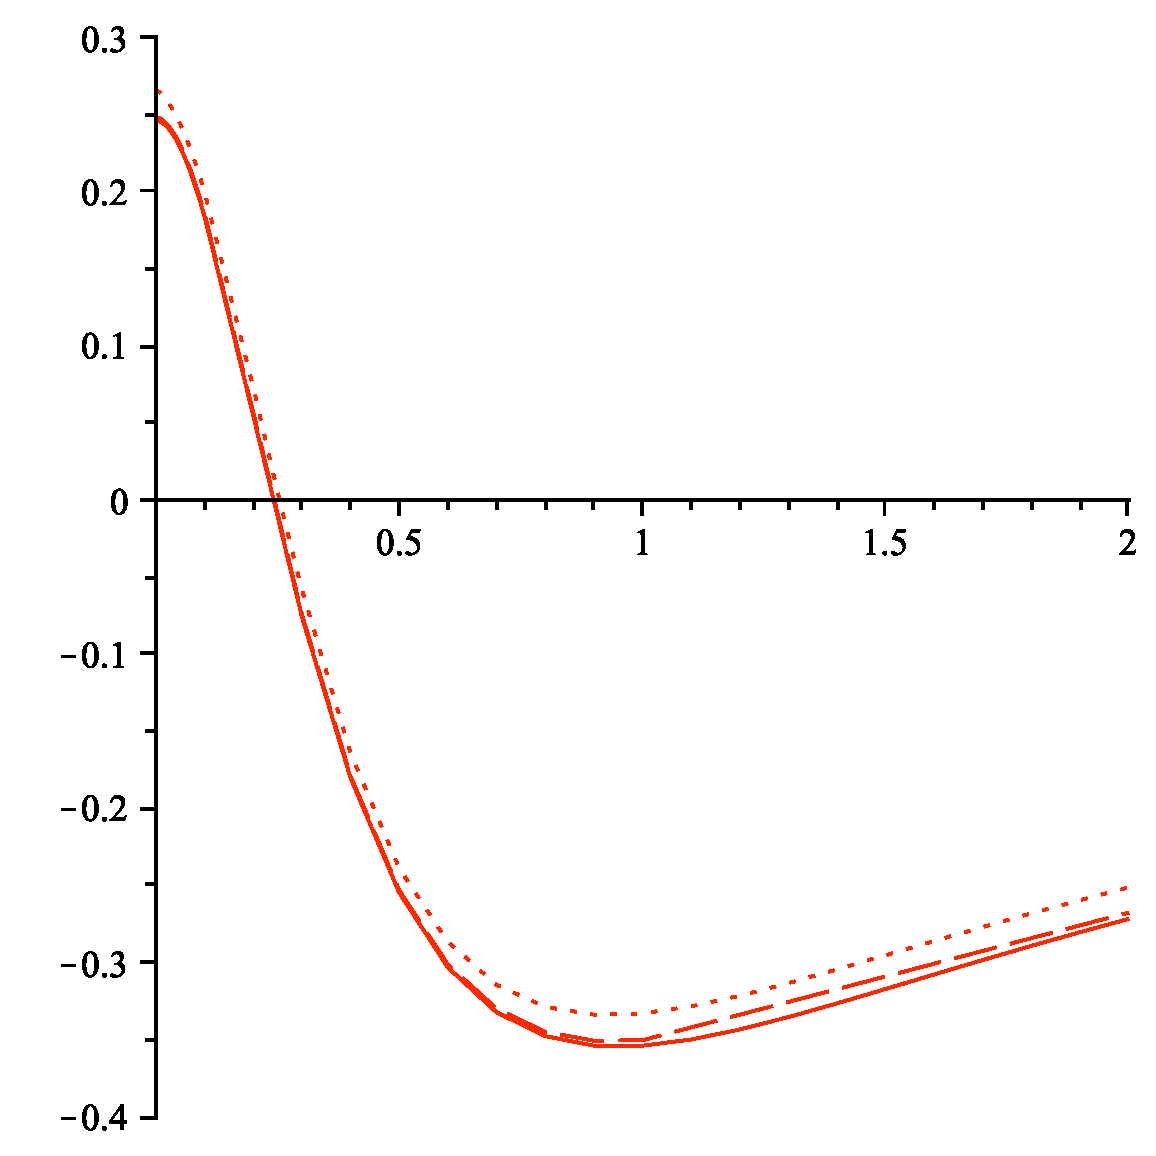
\includegraphics[scale=0.4]{images/graphics/Vacuum_Energy_2.pdf}\\
\small{$\kappa^\vac_\pt$ as a function of $\mpr \pt$\\
for $\N = 1$, $2$ and $3$ (dotted, dashed and solid lines)}
\end{center}
In $\mpr \pt = 0$, we have $\kappa^\vac_\pt \approx 0.266$, $0.248$ and $0.246$ for $\N = 1$, $2$ and $3$ respectively; as $\mpr \pt \to \infty$, we have $\kappa^\vac_\pt \to 0^-$. Since the result converges to an integral expression for $\N \to \infty$, I shall assume that the coefficients obtained by carrying out the computation for $\N = 3$ are already a good approximation.

This energy is represented by following Feynman diagram:
\begin{center}
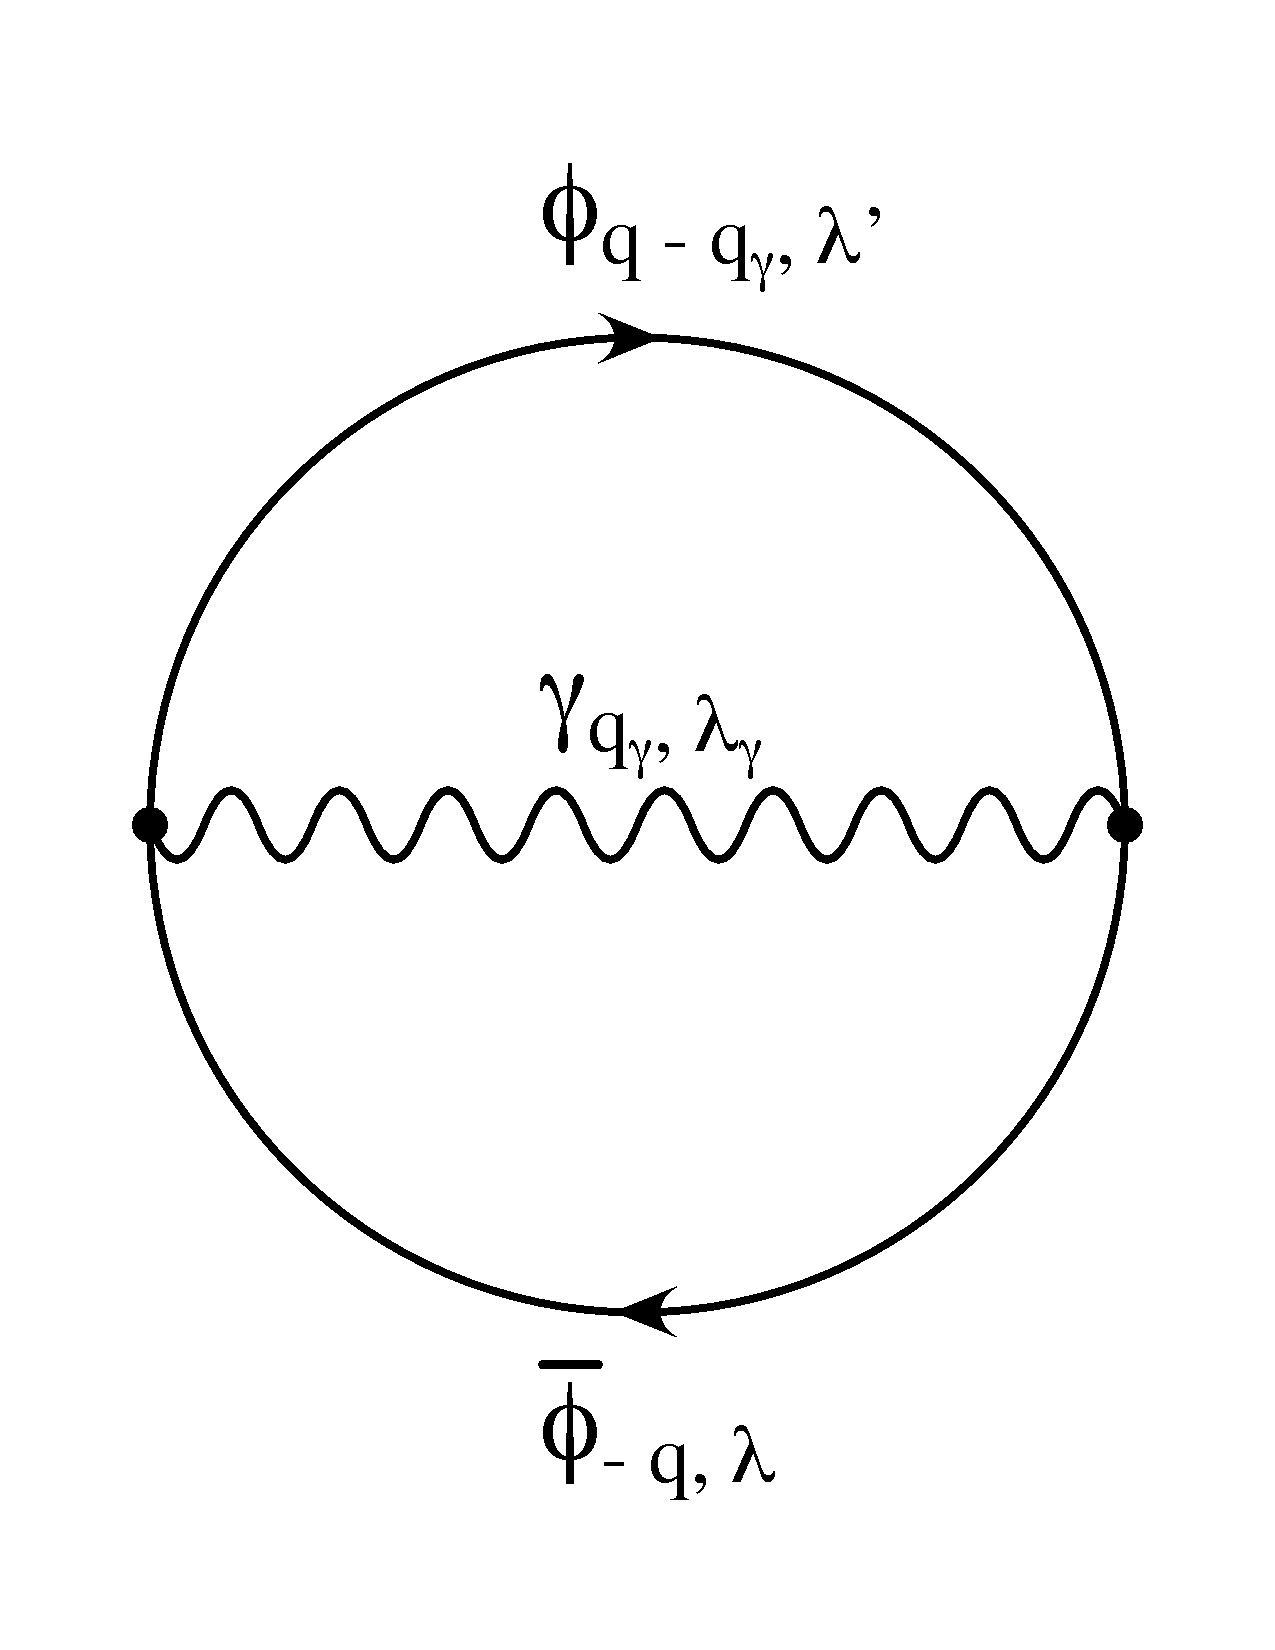
\includegraphics[scale=0.2]{images/diagrams/Vacuum_Energy_2.pdf}
\end{center}
where the Coulomb interaction term is conventionally  represented by the case $\sp_\photon = 0$.
Assuming $\kappa^\vac_\pt \approx 0.25$ for electrically charged fermions, the energy of the electromagnetically dressed vacuum evaluates up to the second order to:
\begin{equation*}
E^{(2)} \approx 0.25 ( 1 + 2 \N )^3 \frac {14} 3 \frac{\e^2}{4 \pi \vpty \a}
\end{equation*}

\section{Dressed charged fermion}

%TODO: Degenerate case! Correct formulas.

We consider an electrically charged fermion of type $\ptf$ in the bare state $\ket{\bQ 1 {\ptf} {\q_\ptf} {\sp_\ptf}}$. Up to the first order, the corresponding dressed state is composed of the bare state, of states of the form $\ket{\bQ 1 {\ptf} {\q_\ptf} {\sp_\ptf} \bQ 1 \pt {\eqp{\q-\q_\photon}} {\sp'} \bQ 1 {\antiparticle \pt} {-\q} \sp \bQ 1 \photon {\q_\photon} {\sp_\photon}}$, where $\pt$ is any electrically charged fermion, $\q_\photon \neq \sv 0$ and $(\pt, \q-\q_\photon, \sp') \neq (\ptf, \q_\ptf, \sp_\ptf)$, as well as of states of the form $\ket{\bQ 1 {\ptf} {\eqp{\q_\ptf - \q_\photon}} \sp \bQ 1 \photon {\q_\photon} {\sp_\photon}}$, where $\q_\photon \neq \sv 0$. The corresponding unnormalized coefficients  are given by:
\begin{equation*}
\FT \Phi^{(1)} = - \sqrt{\frac{\e^2}{4 \pi \vpty \h \c}} ( 1 + 2 \N )^{-3/2} \Qp \pt \frac{\ddirspin \pt {\q - \q_\photon} {\sp'} \gammat 0 \gamvec \dirspin {\antiparticle \pt} {-\q} \sp \ssp \cphotonspin {\q_\photon} {\sp_\photon}}{( 2 \pi q_\photon )^{1 / 2} \left( \Ek \pt {\q - \q_\photon} + \Ek {\antiparticle \pt} {-\q} + \Ek \photon {\q_\photon} \right) \a / \h \c}
\end{equation*}
for states of the form $\ket{\bQ 1 {\ptf} {\q_\ptf} {\sp_\ptf} \bQ 1 \pt {\eqp{\q-\q_\photon}} {\sp'} \bQ 1 {\antiparticle \pt} {-\q} \sp \bQ 1 \photon {\q_\photon} {\sp_\photon}}$, and by:
\begin{equation*}
\FT \Phi^{(1)} = - \sqrt{\frac{\e^2}{4 \pi \vpty \h \c}} ( 1 + 2 \N )^{-3/2} \Qp \ptf \frac{\ddirspin \ptf {\q_\ptf - \q_\photon} \sp \gammat 0 \gamvec \dirspin \ptf {\q_\ptf} {\sp_\ptf} \ssp \cphotonspin {\q_\photon} {\sp_\photon}}{( 2 \pi q_\photon )^{1 / 2} \left( \Ek \ptf {\q_\ptf - \q_\photon} + \Ek \photon {\q_\photon} - \Ek \ptf {\q_\ptf} \right) \a / \h \c}
\end{equation*}
for states of the form $\ket{\bQ 1 {\ptf} {\eqp{\q_\ptf - \q_\photon}} \sp \bQ 1 \photon {\q_\photon} {\sp_\photon}}$, respectively.

The corresponding energy is of second order and can be written as:
\begin{eqnarray*}
E^{(2)} & = & E^{(2)} \left( \vac \right) + \frac{\e^2}{4 \pi \vpty \a} \Qp \ptf^2 \kappa^\ptf_{\q_\ptf, \sp_\ptf} \\
\kappa^\ptf_{\q_\ptf, \sp_\ptf} & \eqdef & ( 1 + 2 \N )^{-3} \sum_{\q_\photon \neq \sv 0} \left[ \frac 1 {2 \pi q_\photon^2} \sum_\sp \left| \ddirspin \ptf {\q_\ptf - \q_\photon} \sp \dirspin \ptf {\q_\ptf} {\sp_\ptf} \right|^2 \right. \\
&& \left. - \frac {\sum_{\sp,\sp_\photon} \left| \ddirspin \ptf {\q_\ptf - \q_\photon} \sp \gammat 0 \gamvec \dirspin \ptf {\q_\ptf} {\sp_\ptf} \ssp \cphotonspin {\q_\photon} {\sp_\photon} \right|^2} {2 \pi q_\photon \left( \Ek \ptf {\q_\ptf - \q_\photon} + \Ek \photon {\q_\photon} - \Ek \ptf {\q_\ptf} \right) \a / \h \c} \right] \\
&& - ( 1 + 2 \N )^{-3} \sum_{\q_\photon \neq \sv 0} \left[ \frac 1 {2 \pi q_\photon^2} \sum_\sp \left| \ddirspin \ptf {\q_\ptf} {\sp_\ptf} \dirspin {\antiparticle \ptf} {-\q_\ptf - \q_\photon} \sp \right|^2 \right. \\
&& \left. - \frac {\sum_{\sp,\sp_\photon} \left| \ddirspin \ptf {\q_\ptf} {\sp_\ptf} \gammat 0 \gamvec \dirspin {\antiparticle \ptf} {-\q_\ptf - \q_\photon} \sp \ssp \cphotonspin {\q_\photon} {\sp_\photon} \right|^2} {2 \pi q_\photon \left( \Ek \ptf {\q_\ptf} + \Ek {\antiparticle \ptf} {-\q_\ptf - \q_\photon} + \Ek \photon {\q_\photon} \right) \a / \h \c} \right]
\end{eqnarray*}
where $E^{(2)} \left( \vac \right)$ is the second order energy of the dressed vacuum. The spin summations evaluate to:
\begin{eqnarray*}
\sum_{\sp} \left| \ddirspin \ptf {\q_\ptf - \q_\photon} \sp \dirspin \ptf {\q_\ptf} {\sp_\ptf} \right|^2 & = & \frac 1 2 \left( 1 + \frac{\mpr \ptf^2 + \eqp{\q_\ptf - \q_\photon} \ssp \q_\ptf}{\Ek \ptf {\q_\ptf - \q_\photon} \Ek \ptf {\q_\ptf} ( \a / \h \c )^2} \right) \\
\sum_{\sp,\sp_\photon} \left| \ddirspin \ptf {\q_\ptf - \q_\photon} \sp \gammat 0 \gamvec \dirspin \ptf {\q_\ptf} {\sp_\ptf} \ssp \cphotonspin {\q_\photon} {\sp_\photon} \right|^2 & = & 1 - \frac{\mpr \ptf^2 + ( \eqp{\q_\ptf - \q_\photon} \ssp \q_\photon ) ( \q_\ptf \ssp \q_\photon ) / q_\photon^2}{\Ek \ptf {\q_\ptf - \q_\photon} \Ek \ptf {\q_\ptf} ( \a / \h \c )^2} \\
\sum_{\sp} \left| \ddirspin \ptf {\q_\ptf} {\sp_\ptf} \dirspin {\antiparticle \ptf} {-\q_\ptf - \q_\photon} \sp \right|^2 & = & \frac 1 2 \left( 1 - \frac{\mpr \ptf^2 + \q_\ptf \ssp \eqp{\q_\ptf + \q_\photon}}{\Ek \ptf {\q_\ptf} \Ek {\antiparticle \ptf} {-\q_\ptf - \q_\photon} ( \a / \h \c )^2} \right) \\
\sum_{\sp,\sp_\photon} \left| \ddirspin \ptf {\q_\ptf} {\sp_\ptf} \gammat 0 \gamvec \dirspin {\antiparticle \ptf} {-\q_\ptf - \q_\photon} \sp \ssp \cphotonspin {\q_\photon} {\sp_\photon} \right|^2 & = & 1 + \frac{\mpr \ptf^2 + ( \q_\ptf \ssp \q_\photon ) ( \eqp{\q_\ptf + \q_\photon} \ssp \q_\photon ) / q_\photon^2}{\Ek \ptf {\q_\ptf} \Ek {\antiparticle \ptf} {- \q_\ptf - \q_\photon} ( \a / \h \c )^2}
\end{eqnarray*}
The vacuum energy diagram is also completed by subtracting following contribution:
\begin{center}
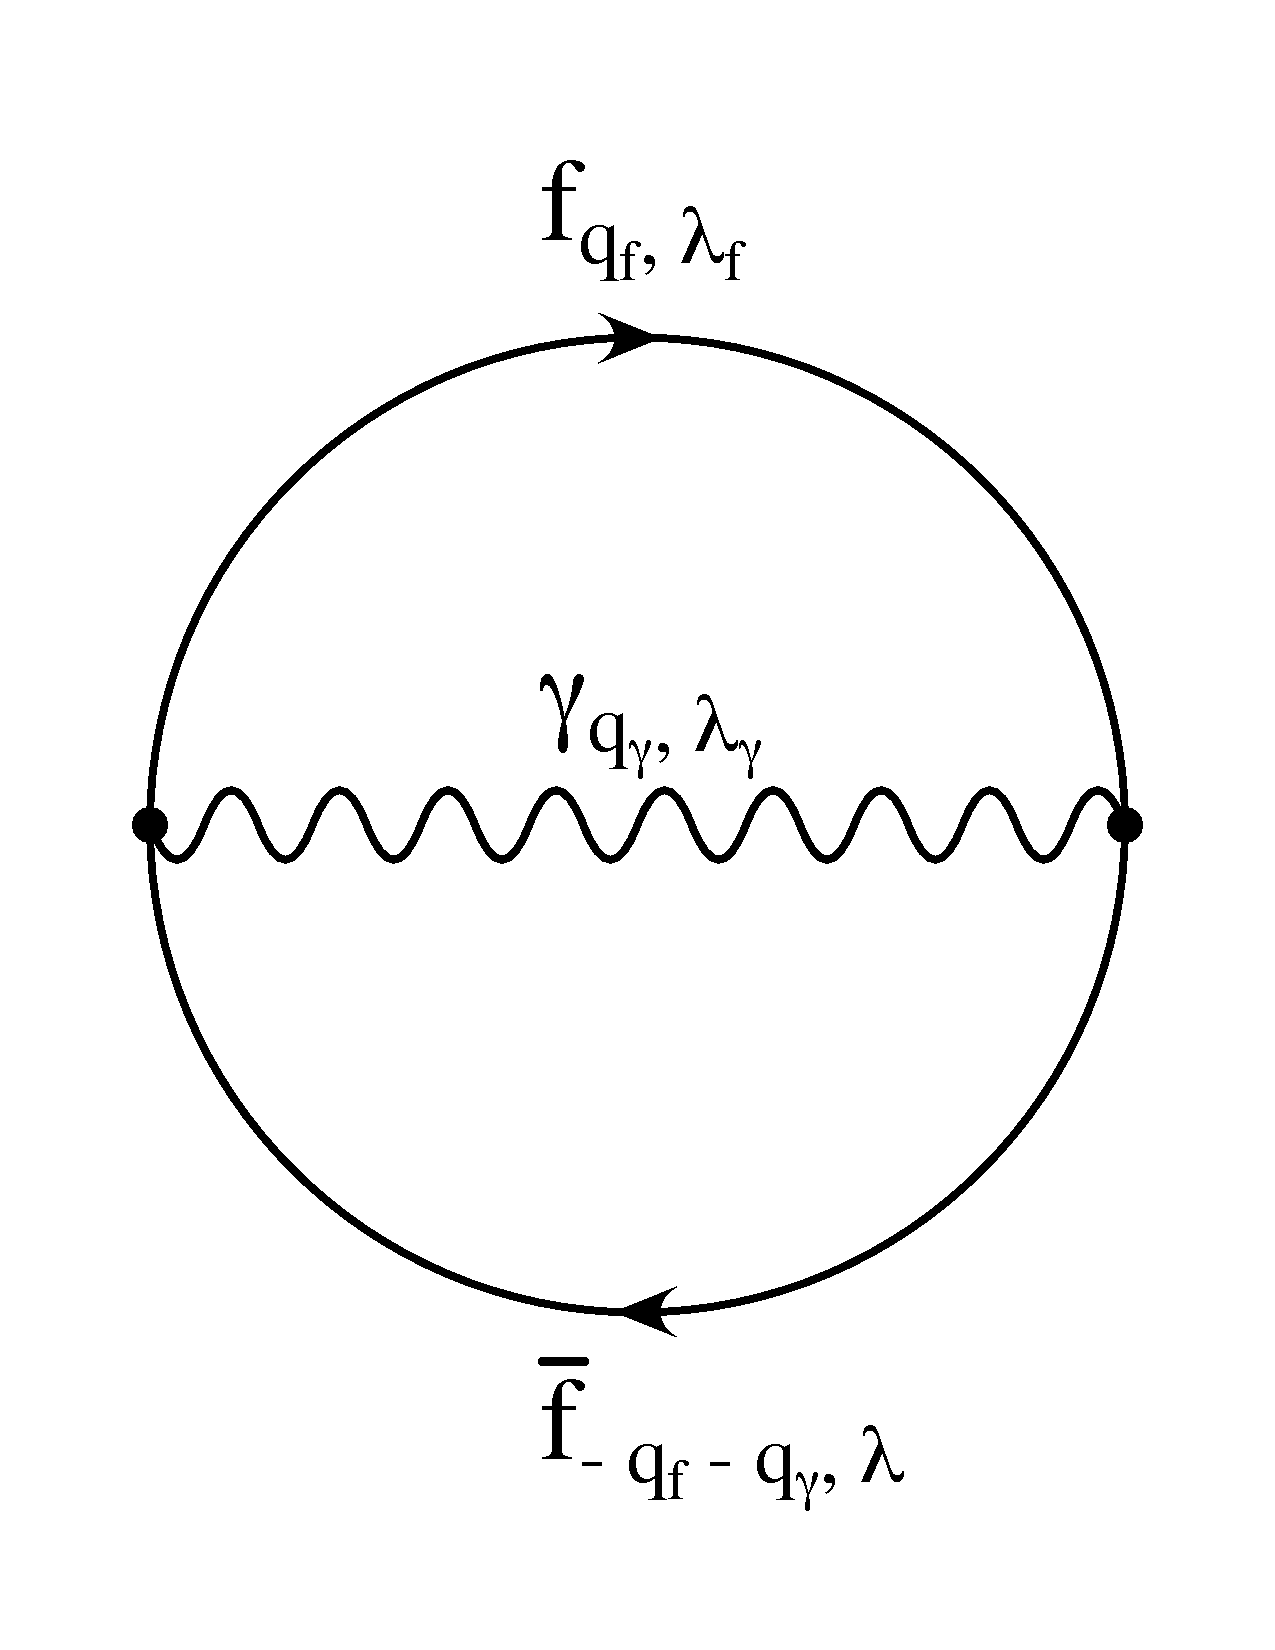
\includegraphics[scale=0.2]{images/diagrams/Charged_Fermion_Energy_2a.pdf}
\end{center}
and by adding following self-energy diagram:
\begin{center}
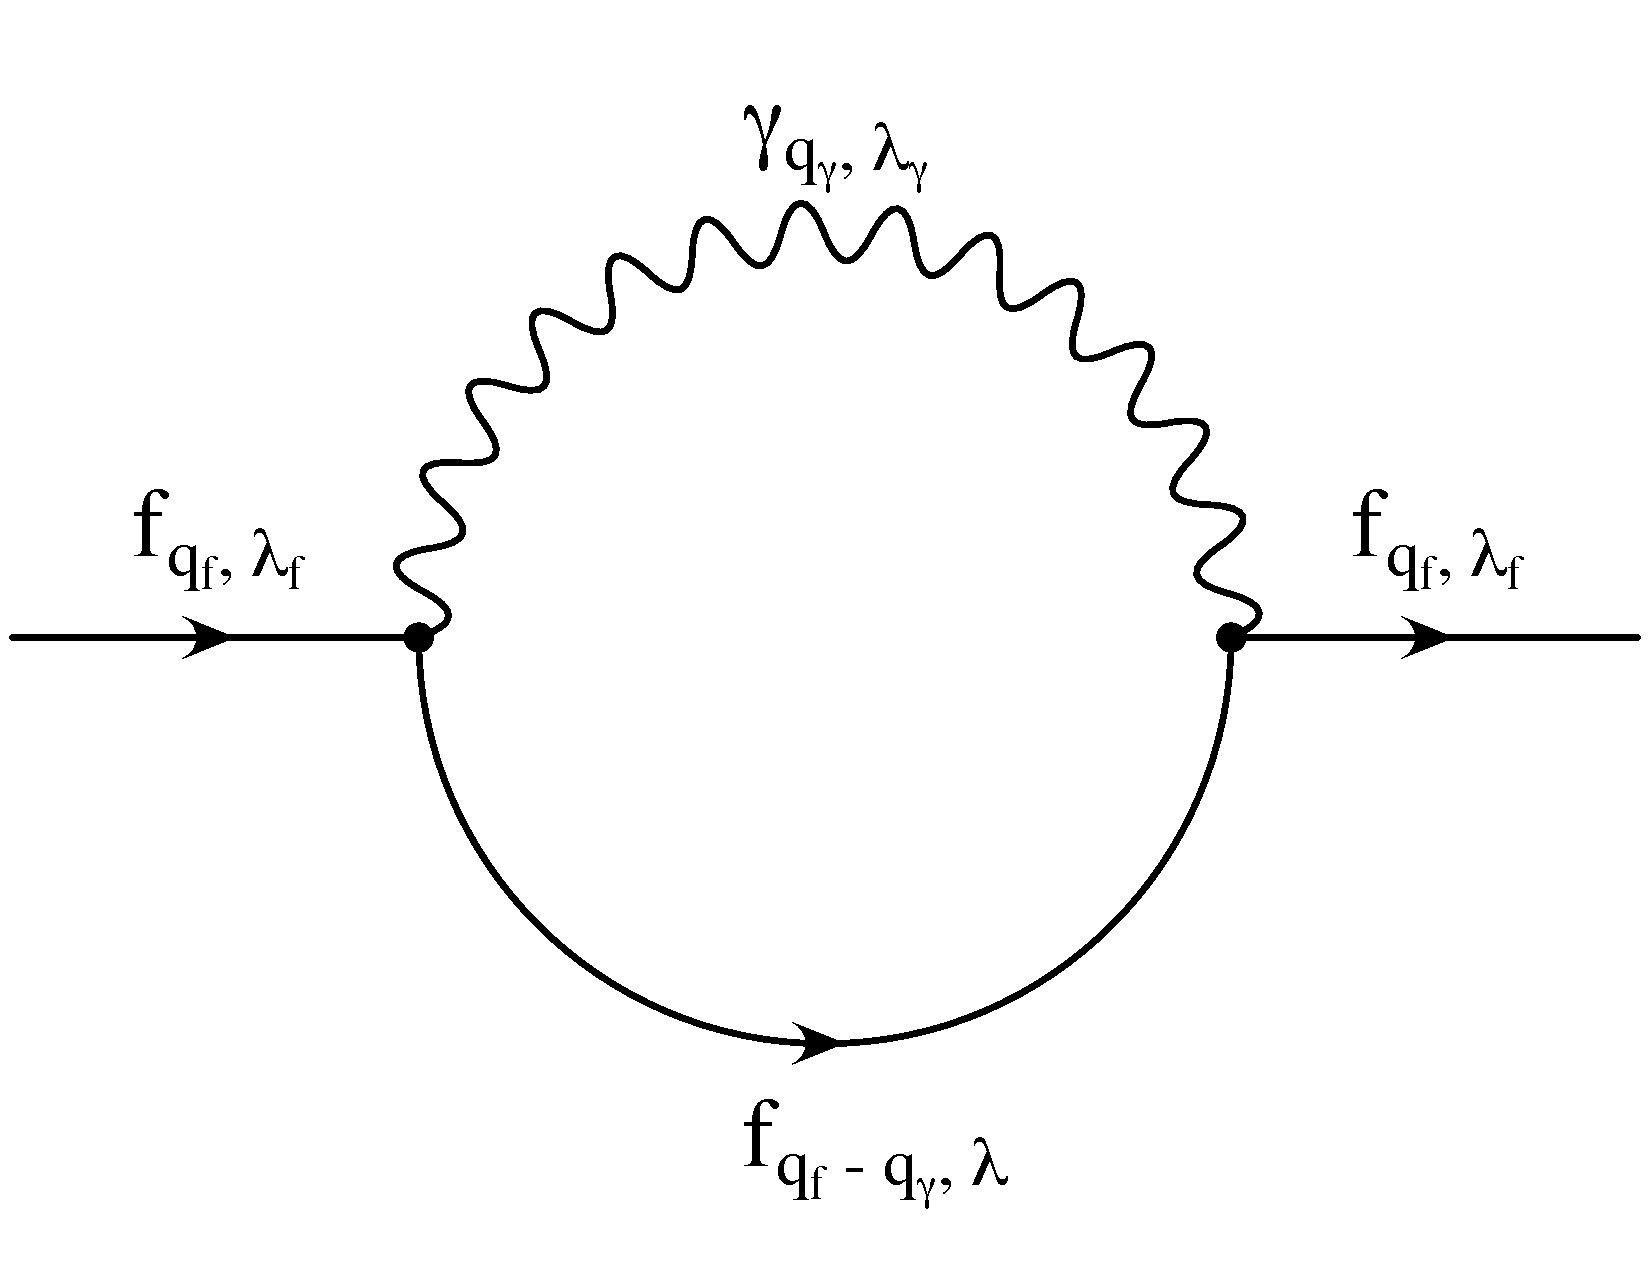
\includegraphics[scale=0.24]{images/diagrams/Charged_Fermion_Energy_2b.pdf}
\end{center}
for a given mode $(\q_\ptf, \sp_\ptf)$ of the fermion field.
%TODO: Evaluate at \q_\ptf = 0.

\section{Dressed photon}

We consider a photon in the bare state $\ket{\bQ 1 {\photon} {\q_ \photon} {\sp_ \photon}}$, where $\q_\photon \neq \sv 0$. Up to the first order, the corresponding dressed state is composed of the bare state, of states of the form $\ket{\bQ 1 {\photon} {\q_ \photon} {\sp_ \photon} \bQ 1 \pt {\eqp{\q-\q_\photon'}} {\sp'} \bQ 1 {\antiparticle \pt} {-\q} \sp \bQ 1 \photon {\q_\photon'} {\sp_\photon'}}$, where $\pt$ is any electrically charged fermion, $\q_\photon' \neq \sv 0$ and $(\q_\photon',\sp_\photon') \neq (\q_ \photon,\sp_ \photon)$, of states of the form $\ket{\bQ 2 {\photon} {\q_ \photon} {\sp_ \photon} \bQ 1 \pt {\eqp{\q-\q_\photon}} {\sp'} \bQ 1 {\antiparticle \pt} {-\q} \sp}$ as well as of states of the form $\ket{\bQ 1 {\pt} {\eqp{\q + \q_\photon}} {\sp'} \bQ 1 {\antiparticle \pt} {-\q} \sp}$. The corresponding unnormalized coefficients  are given by:
\begin{equation*}
\FT \Phi^{(1)} = - \sqrt{\frac{\e^2}{4 \pi \vpty \h \c}} ( 1 + 2 \N )^{-3/2} \Qp \pt \frac{\ddirspin \pt {\q - \q_\photon'} {\sp'} \gammat 0 \gamvec \dirspin {\antiparticle \pt} {-\q} \sp \ssp \cphotonspin {\q_\photon'} {\sp_\photon'}}{( 2 \pi q_\photon' )^{1 / 2} \left( \Ek \pt {\q - \q_\photon'} + \Ek {\antiparticle \pt} {-\q} + \Ek \photon {\q_\photon'} \right) \a / \h \c}
\end{equation*}
for states of the form $\ket{\bQ 1 {\photon} {\q_ \photon} {\sp_ \photon} \bQ 1 \pt {\eqp{\q-\q_\photon'}} {\sp'} \bQ 1 {\antiparticle \pt} {-\q} \sp \bQ 1 \photon {\q_\photon'} {\sp_\photon'}}$, by:
\begin{equation*}
\FT \Phi^{(1)} = - \sqrt{2 \frac{\e^2}{4 \pi \vpty \h \c}} ( 1 + 2 \N )^{-3/2} \Qp \pt \frac{\ddirspin \pt {\q - \q_\photon} {\sp'} \gammat 0 \gamvec \dirspin {\antiparticle \pt} {-\q} \sp \ssp \cphotonspin {\q_\photon} {\sp_\photon}}{( 2 \pi q_\photon )^{1 / 2} \left( \Ek \pt {\q - \q_\photon} + \Ek {\antiparticle \pt} {-\q} + \Ek \photon {\q_\photon} \right) \a / \h \c}
\end{equation*}
for states of the form $\ket{\bQ 2 {\photon} {\q_ \photon} {\sp_ \photon} \bQ 1 \pt {\eqp{\q-\q_\photon'}} {\sp'} \bQ 1 {\antiparticle \pt} {-\q} \sp}$, and by:
\begin{equation*}
\FT \Phi^{(1)} = - \sqrt{\frac{\e^2}{4 \pi \vpty \h \c}} ( 1 + 2 \N )^{-3/2} \Qp \pt \frac{\ddirspin \pt {\q + \q_\photon} {\sp'} \gammat 0 \gamvec \dirspin {\antiparticle \pt} {-\q} \sp \ssp \photonspin {\q_\photon} {\sp_\photon}}{( 2 \pi q_\photon )^{1 / 2} \left( \Ek \pt {\q + \q_\photon} + \Ek {\antiparticle \pt} {-\q} - \Ek \photon {\q_\photon} \right) \a / \h \c}
\end{equation*}
for states of the form $\ket{\bQ 1 {\pt} {\eqp{\q + \q_\photon}} {\sp'} \bQ 1 {\antiparticle \pt} {-\q} \sp}$, respectively.

The corresponding energy is of second order and can be written as:
\begin{eqnarray*}
E^{(2)} & = & E^{(2)} \left( \vac \right) - \frac{\e^2}{4 \pi \vpty \a} \sum_{\pt} \Qp \pt^2 \kappa^{\photon}_{\q_\photon,\sp_\photon,\pt} \\
\kappa^{\photon}_{\q_\photon,\sp_\photon,\pt} & \eqdef & ( 1 + 2 \N )^{-3} \sum_{\q} \frac {\sum_{\sp',\sp} \left| \ddirspin \pt {\q - \q_\photon} {\sp'} \gammat 0 \gamvec \dirspin {\antiparticle \pt} {-\q} \sp \ssp \cphotonspin {\q_\photon} {\sp_\photon} \right|^2} {2 \pi q_\photon \left( \Ek \pt {\q - \q_\photon} + \Ek {\antiparticle \pt} {-\q} + \Ek \photon {\q_\photon} \right) \a / \h \c} \\
&& + ( 1 + 2 \N )^{-3} \sum_{\q} \frac {\sum_{\sp',\sp} \left| \ddirspin \pt {\q + \q_\photon} {\sp'} \gammat 0 \gamvec \dirspin {\antiparticle \pt} {-\q} \sp \ssp \photonspin {\q_\photon} {\sp_\photon} \right|^2} {2 \pi q_\photon \left( \Ek \pt {\q + \q_\photon} + \Ek {\antiparticle \pt} {-\q} - \Ek \photon {\q_\photon} \right) \a / \h \c}
\end{eqnarray*}
where the spin summations evaluate to:
\begin{eqnarray*}
\sum_{\sp',\sp} \left| \ddirspin \pt {\q - \q_\photon} {\sp'} \gammat 0 \gamvec \dirspin {\antiparticle \pt} {-\q} \sp \ssp \cphotonspin {\q_\photon} {\sp_\photon} \right|^2 & = & 1 + \frac{\mpr \pt^2 + ( \eqp{\q - \q_\photon} \ssp \q_\photon ) ( \q \ssp \q_\photon ) / q_\photon^2}{\Ek \pt {\q - \q_\photon} \Ek {\antiparticle \pt} {-\q} ( \a / \h \c )^2} \\
\sum_{\sp',\sp} \left| \ddirspin \pt {\q + \q_\photon} {\sp'} \gammat 0 \gamvec \dirspin {\antiparticle \pt} {-\q} \sp \ssp \photonspin {\q_\photon} {\sp_\photon} \right|^2 & = & 1 + \frac{\mpr \pt^2 + ( \eqp{\q + \q_\photon} \ssp \q_\photon ) ( \q \ssp \q_\photon ) / q_\photon^2}{\Ek \pt {\q + \q_\photon} \Ek {\antiparticle \pt} {-\q} ( \a / \h \c )^2}
\end{eqnarray*}
The vacuum energy diagram is also completed by adding following (negative) contribution:
\begin{center}
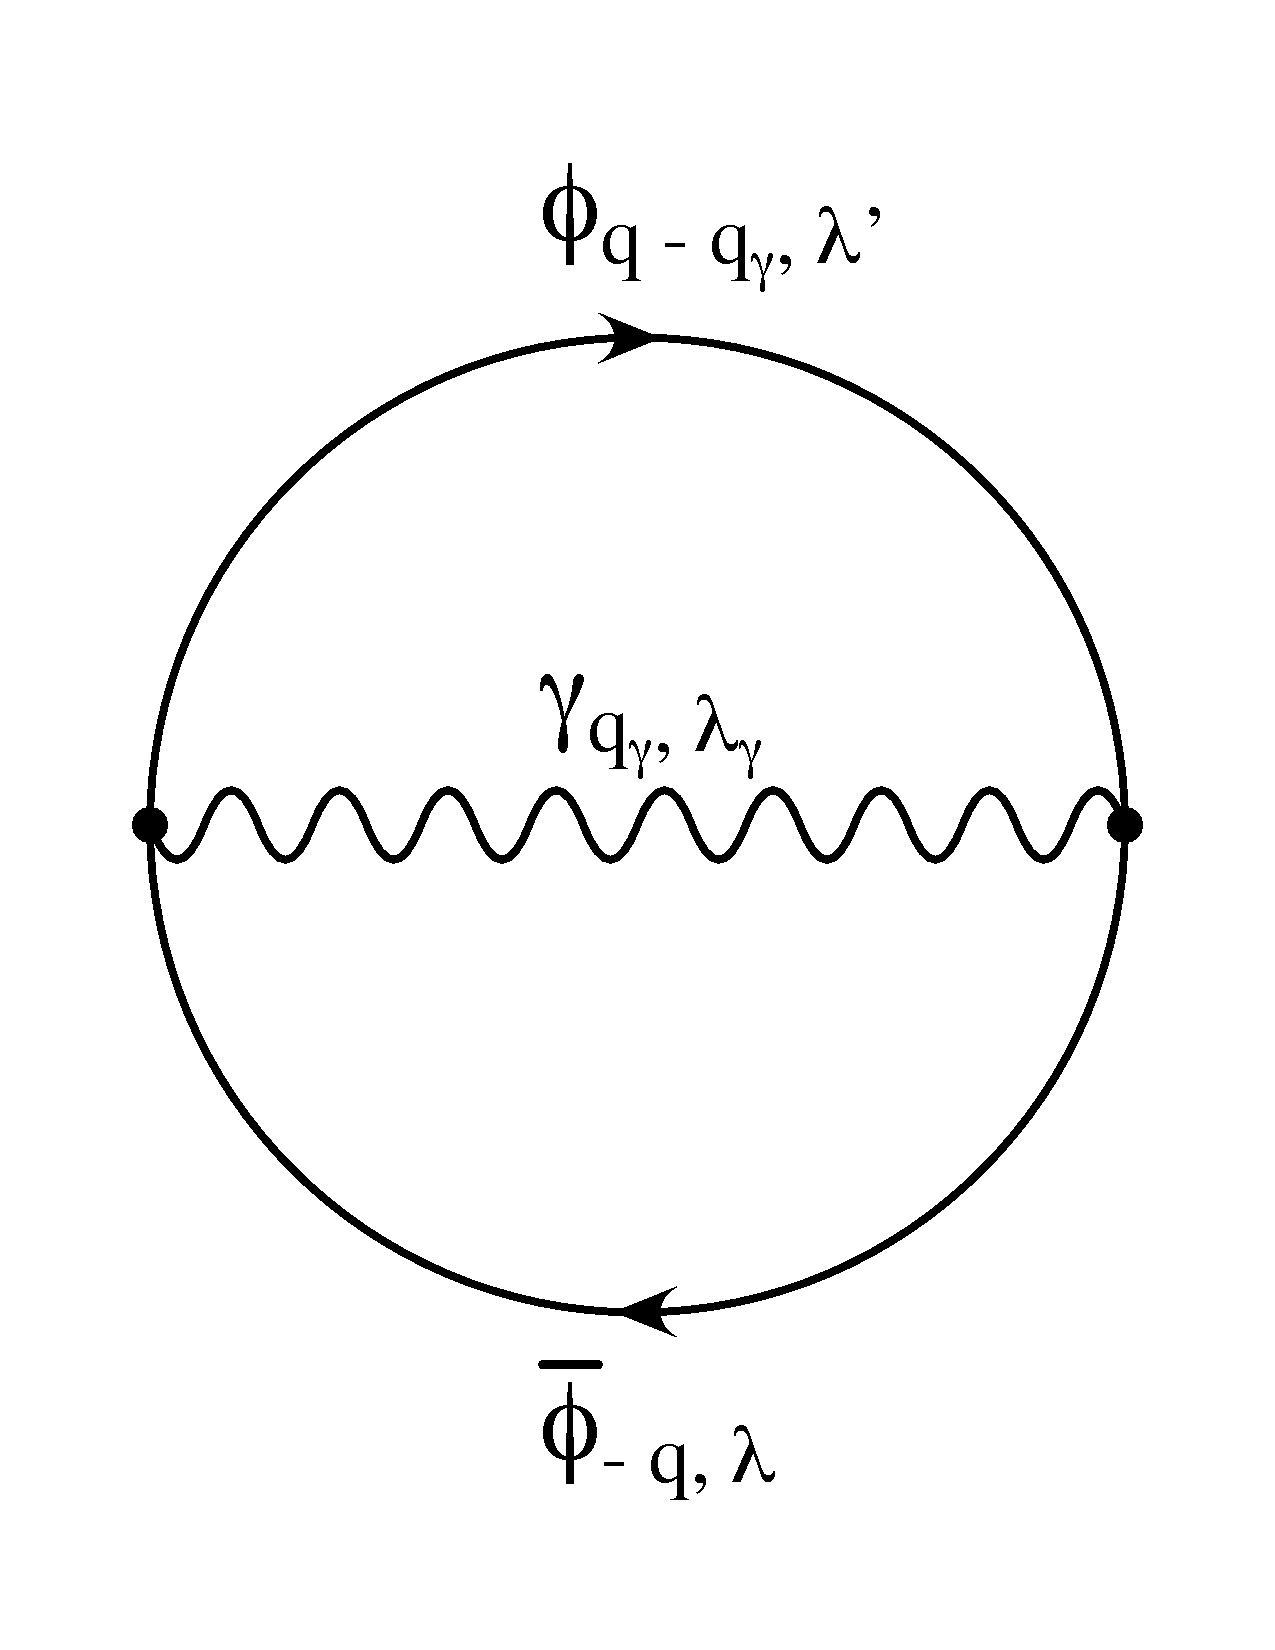
\includegraphics[scale=0.2]{images/diagrams/Photon_Energy_2a.pdf}
\end{center}
and by adding following (negative) self-energy diagram:
\begin{center}
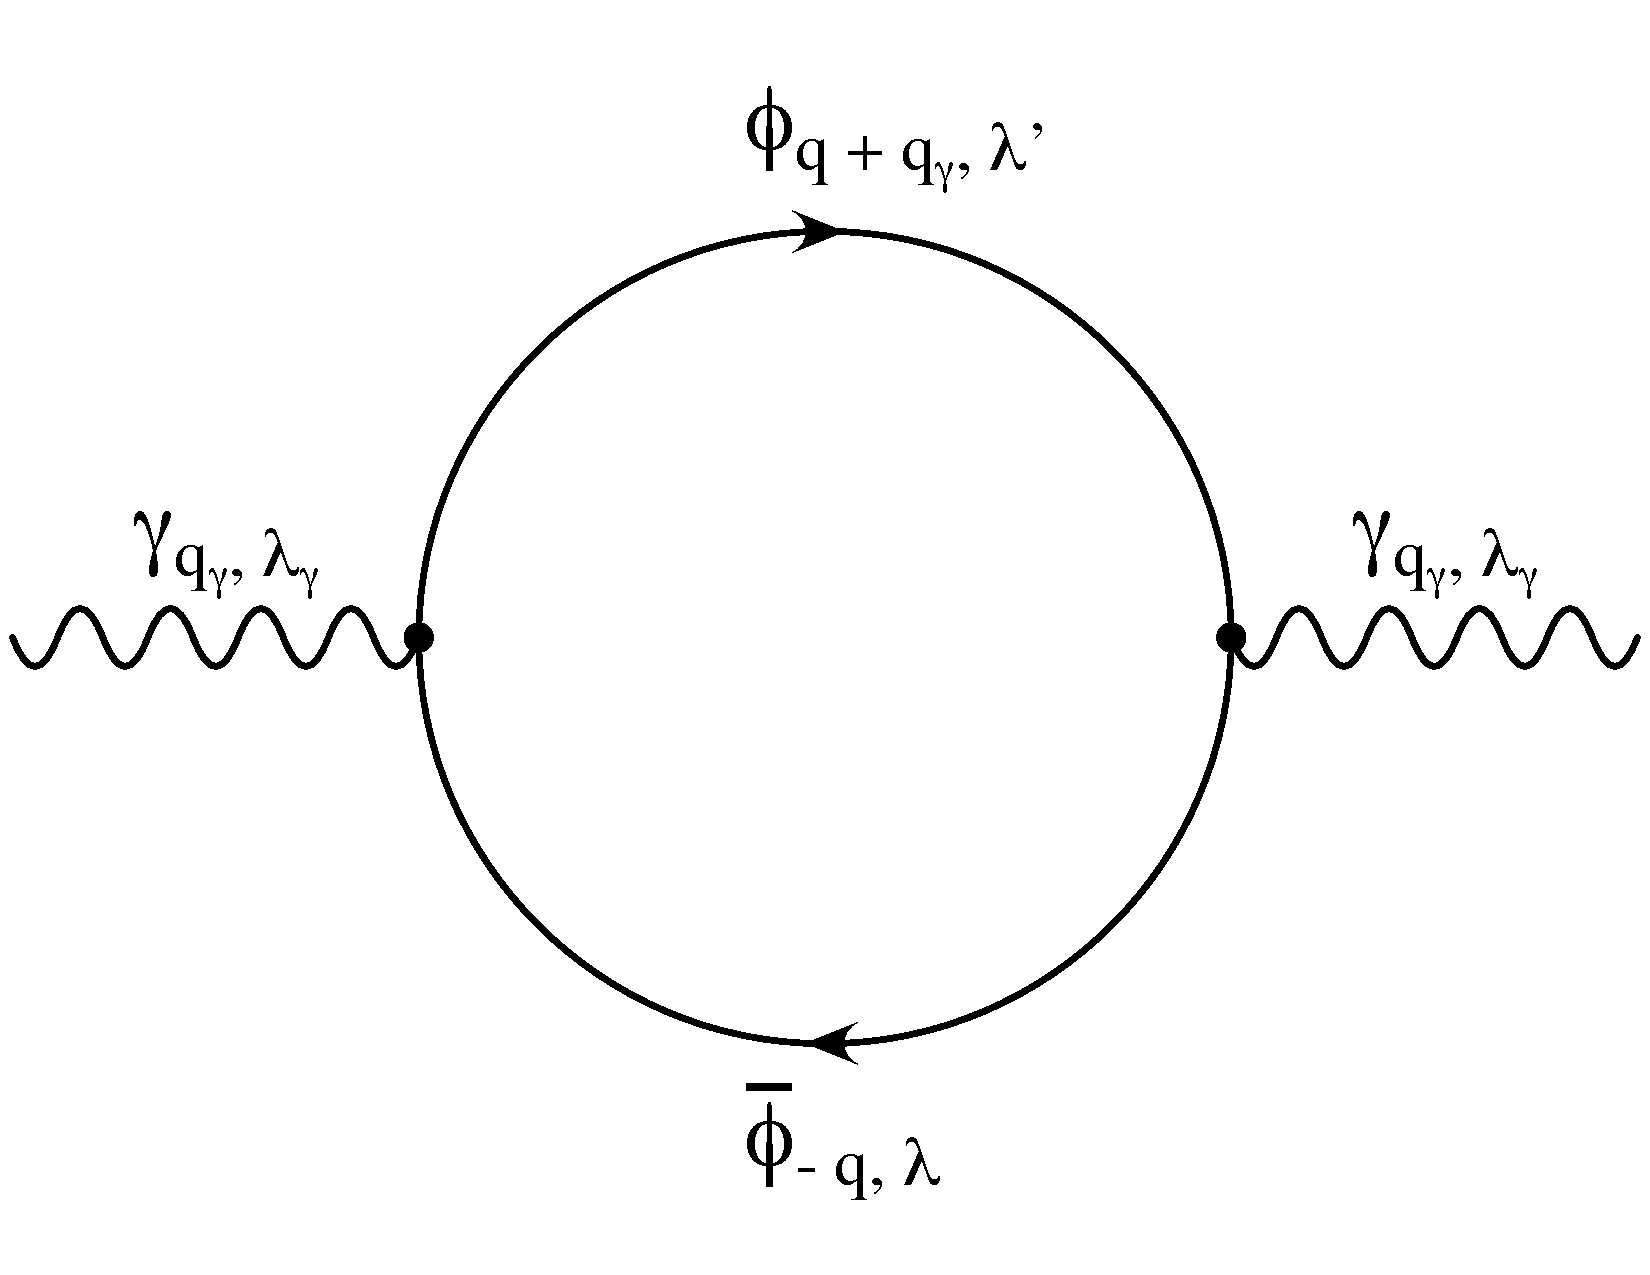
\includegraphics[scale=0.24]{images/diagrams/Photon_Energy_2b.pdf}
\end{center}
for a given mode $(\q_\photon, \sp_\photon)$ of the photon field.

\part{Examples}

\chapter{Wave packets}
\label{Wave packets}

\section{Gaussian wave packet}

A well-known consequence of the quantum formalism is the impossibility to describe a particle, like in classical mechanics, as a mass point having at each instant a well-defined position and velocity. In the quantum mechanics of a single particle in continuous space-time, the movement of the wave packet defining its statistical position can still be described, like in classical fluid mechanics, by a probability current density (which is related to the phase gradient of the wave packet), but as soon as several particles are present or are even being created and annihilated like in Quantum Field Theory, the analogy to classical fluid mechanics becomes much more elusive. It is still possible, however, to describe approximate particle trajectories in the frame of Quantum Field Theory if one considers that proper quantum effects may remain beyond the reach of experimental precision in some situations. Gaussian wave packets are a typical model of such particles with a quasi-classical behavior, i.e. with a position and a velocity being well-defined to a good approximation.

A Gaussian wave packet of a particle of type $\pt$ and in the spin state $\sp$, with a mean momentum $\q_0 \in (\IZ/(1+2\N))^3$, a mean position $\n_0 \in \IR^3$ and a width $w_0 \in \IR_+^*$, is given by:
\begin{eqnarray*}
\ket \Psi & = & \dop{G^\pt_\sp}(\q_0,\n_0,w_0) \ket \vac \\
\dop{G^\pt_\sp}(\q_0,\n_0,w_0) & \eqdef & C(\q_0,w_0) (2w_0)^{3/2} (1+2\N)^{-3/2} \\
&& \sum_{\q} \exp{-2 \pi w_0^2 \q^2 - \i 2 \pi \q \ssp \n_0} \cop\pt{\q_0+\q}\sp
\end{eqnarray*}
with the normalization factor:
\begin{equation*}
C(\q_0,w_0) \eqdef \left[ (2w_0)^3 (1+2\N)^{-3} \sum_{\q} \exp{-4 \pi w_0^2 \q^2} \right]^{-1/2}
\end{equation*}
In the usual case where $1 \ll w_0 \ll \N$, this normalization factor approximates to 1. On the position basis, the creation operator of the Gaussian wave packet can be expressed as:
\begin{eqnarray*}
\dop{G^\pt_\sp}(\q_0,\n_0,w_0) & = & C(\q_0,w_0) w_0^{-3/2} \sum_{\n} A(\n - \n_0'(\n),w_0) \\
&& \exp{-\pi (\n - \n_0'(\n))^2/2 w_0^2 + \i 2 \pi \q_0 \ssp \n} \cop\pt\n\sp
\end{eqnarray*}
with the numerical factor:
\begin{equation*}
A(\n - \n_0'(\n),w_0) \eqdef (2w_0^2)^{3/2} (1+2\N)^{-3} \sum_{\q} \exp{-2 \pi w_0^2 \left( \q - \i (\n - \n_0'(\n))/2 w_0^2 \right)^2}
\end{equation*}
where $\n_0'(\n)$ can be chosen arbitrarily in $\n_0 + ((1+2\N) \IZ)^3$. In the usual case where $1 \ll w_0 \ll \N$, this factor approximates to 1 if $\n_0'(\n)$ can be chosen such as $\| \n-\n_0'(\n) \| \ll \N$. To the zeroth order, the Hamiltonian evolution of the Gaussian wave packet $\ket{\Psi_0} = \dop{G^\pt_\sp}(\q_0,\n_0,w_0) \ket \vac$ is given by:
\begin{eqnarray*}
\ket{\Psi_t} & = & C(\q_0,w_0) (2w_0)^{3/2} (1+2\N)^{-3/2} \\
&& \sum_{\q} \exp{-2 \pi w_0^2 \q^2 - \i 2 \pi \q \ssp \n_0 -\i 2 \pi \Ek \pt {\q_0+\q} (t - t_0) / \h} \cop\pt{\q_0+\q}\sp \ket \vac
\end{eqnarray*}
If $w_0 \gg q_0^{-1}$, the saddle-point approximation $\Ek \pt {\q_0+\q} \approx \Ek \pt {\q_0} + \q \ssp \nabla_{\q} \Ek \pt {\q_0}$ can be used and it follows:
\begin{eqnarray*}
\ket{\Psi_t} & \approx & \exp{-\i 2 \pi \Ek \pt {\q_0} (t - t_0) / \h} \dop{G^\pt_\sp}(\q_0,\n_t,w_0) \ket \vac \\
\n_t & \eqdef & \n_0 + \vk \pt {\q_0} (t - t_0) / \a
\end{eqnarray*}
The mean position $\n_t$ of the particle follows therefore, in the toroidal space $(\IR / (1+2\N)\IZ)^3$,  a classical trajectory at the constant velocity $\vk \pt {\q_0}$ which would be attributed classically to a point mass of mass $\mp \pt$ and of momentum $\h \eqp{\q_0} / \a$.

\chapter{Coulomb scattering}
\label{Coulomb scattering}

\section{Leading order calculation}

We consider in this section the scattering of an electron by an atomic nucleus of atomic number $Z$. We model the nucleus by a classical point charge without magnetic moment, being at rest at the origin in the lattice reference frame and having a mass much higher than the mass of the electron. The corresponding electromagnetic field is described as a classical Coulomb potential $\V^{cl}$ given in terms of Fourier components by:
\begin{eqnarray*}
\V^{cl}_{\n} & \eqdef & ( 1 + 2 \N )^{-3} \sum_{\q_\photon \neq \sv 0} \FT \V^{cl}_{\q_\photon} \exp{\i 2 \pi \n \ssp \q_\photon} \\
\FT \V^{cl}_{\q_\photon} & \eqdef & \frac{Z \e}{4 \pi^2 \vpty \a q_\photon^2}
\end{eqnarray*}
The corresponding semi-classical interaction Hamiltonian takes the form:
\begin{eqnarray*}
\Hop' & \eqdef & \HopQED + \Hop^{cl} \\
\Hop^{cl} & \eqdef & \sum_{\n} \Qop \n \V^{cl}_{\n}
\end{eqnarray*}
and its development on the plane wave basis is given by:
\begin{eqnarray*}
\Hop^{cl} & = & \frac{Z \e^2}{4 \pi^2 \vpty \a} ( 1 + 2 \N )^{-3} \sum_{\pt, \q, \sp', \sp} \Qp \pt \sum_{\q_\photon \neq \sv 0} q_\photon^{-2} \\
&& \left( \SCop \pt {\q + \q_\photon} {\sp'} + \SAop {\antiparticle \pt} {-\q - \q_\photon} {\sp'} \right) \gammat 0 \left( \SAop \pt \q \sp + \SCop {\antiparticle \pt} {-\q} \sp \right)
\end{eqnarray*}

As initial and final states, we take:
\begin{eqnarray*}
\ket{\Psi_i} & \eqdef & \ketX 1 \electron {\q_i} {\sp_i} \\
\ket{\Psi_f} & \eqdef & \ketX 1 \electron {\q_f} {\sp_f}
\end{eqnarray*}
The matrix element of the interaction Hamiltonian is given for $\q_f \neq \q_i$ by:
\begin{equation*}
H'_{f,i} = (1 + 2 \N )^{-3} \frac {-Z \e^2}{4 \pi^2 \vpty \a \norm{\q_f - \q_i}^2} \ddirspin \electron {\q_f} {\sp_f} \dirspin \electron {\q_i} {\sp_i}
\end{equation*}
and the leading order transition probability for this process is also represented by following diagram:
\begin{center}
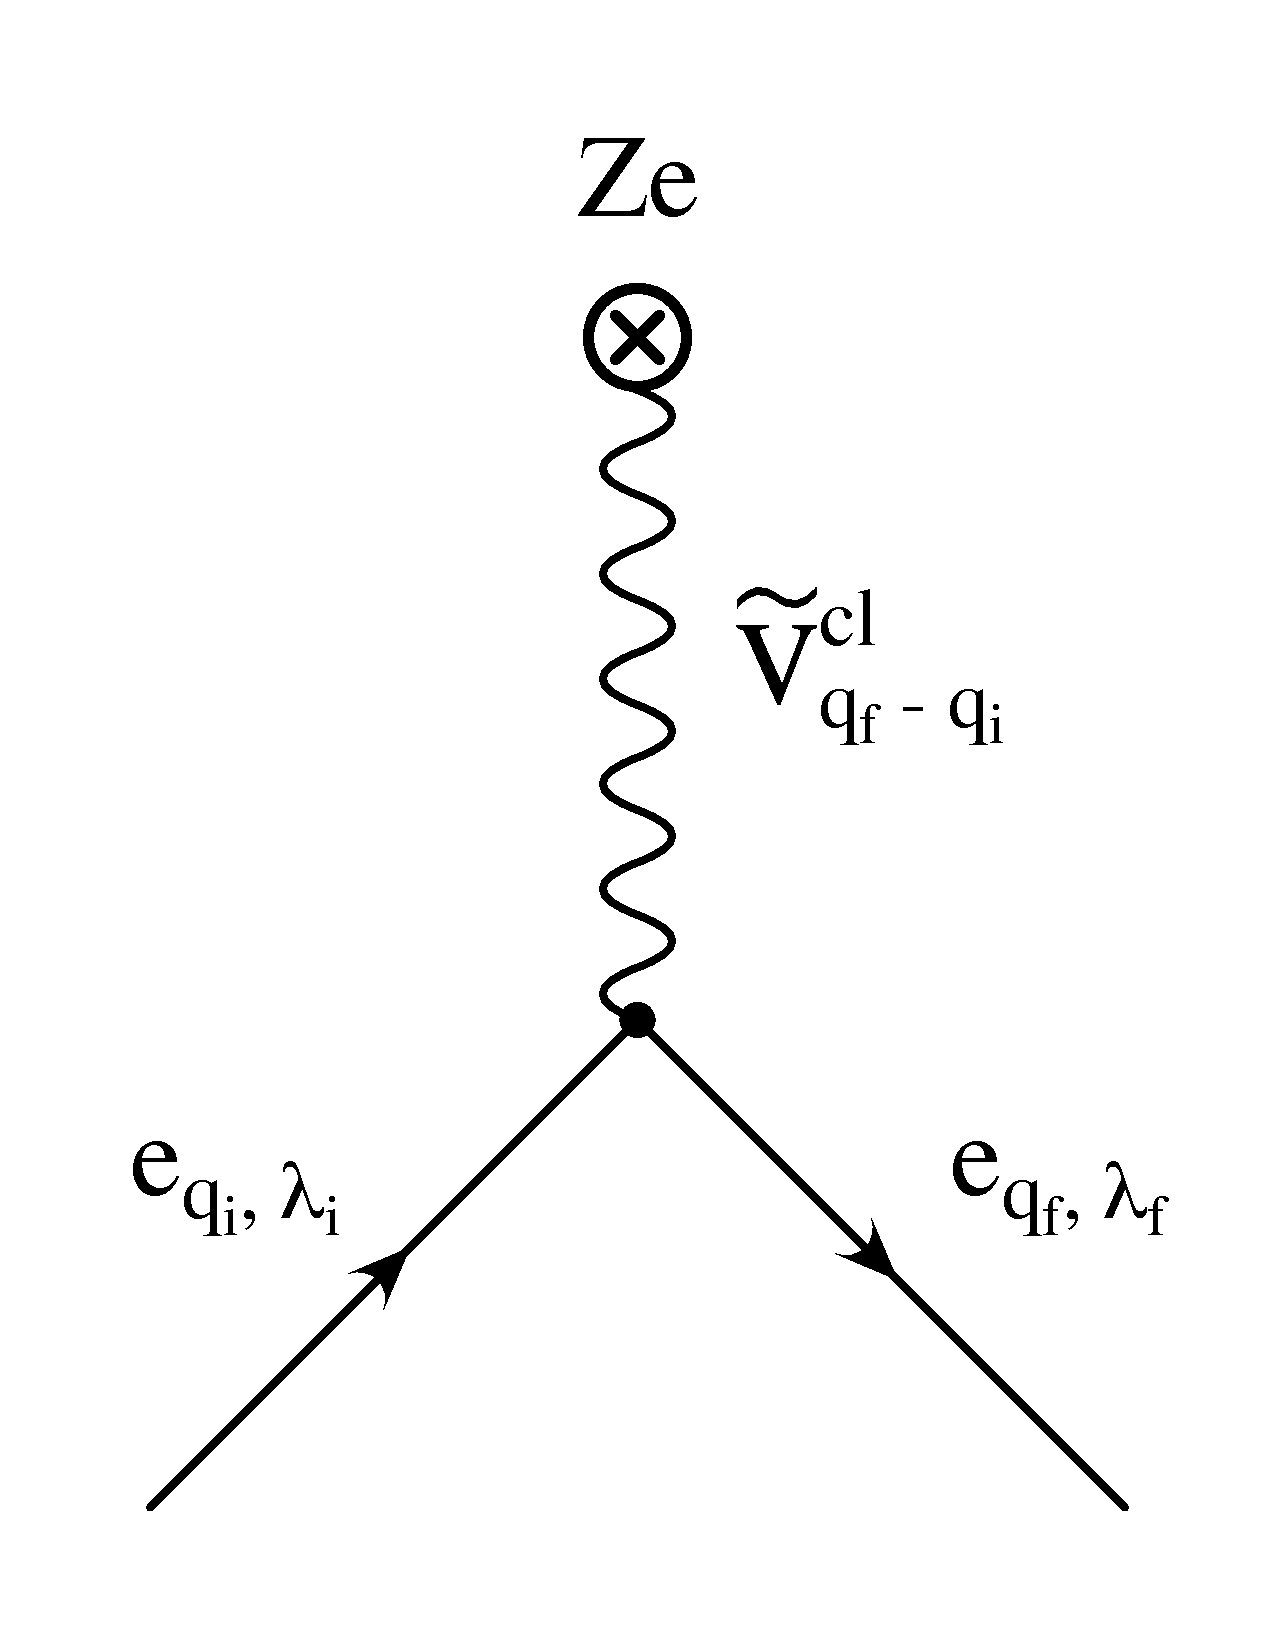
\includegraphics[scale=0.2]{images/diagrams/Coulomb_Scattering.pdf}
\end{center}
We consider a detector capturing the electrons having their momentum in the solid angle $\delta \Omega$. For $i \notin \delta \F$, the leading order transition probability takes the form:
\begin{eqnarray*}
\TPn i {\delta \F} 2 & \approx & \int_{\delta \Omega} \int_0^{\infty} ( 2 \pi )^2 \frac{t - t_0} \h \left| H'_{f + \delta \q,i} \right|^2 \deltaE2{E_{f + \delta \q} - E_i} \\
&& \left( (1 + 2 \N) \frac \a \h \right)^3 p^2 \dnp \dO
\end{eqnarray*}
By taking following continuation for the factors of the integrand:
\begin{eqnarray*}
\left| H'_{f + \delta \q,i} \right|^2 & \approx & \left( (1+2\N) \a \right)^{-6} \frac {Z^2 \e^4 \h^4}{16 \pi^4 \vpty^2 \norm{\p - \p_i}^4} \left| \ddirspin \electron \q {\sp_f} \dirspin \electron {\q_i} {\sp_i} \right|^2 \\
\deltaE2{E_{f + \delta \q} - E_i} & \approx & \deltaE2{\sqrt{(\mp \electron \c^2)^2 + (p \c)^2} - E_i}
\end{eqnarray*}
the integration over $p$ yields to:
\begin{equation*}
\TPn i {\delta \F} 2 \approx (t - t_0) j_i \CSn i {\delta \F} 2
\end{equation*}
where $\sv j_i$ is the incident particle flux, given by:
\begin{eqnarray*}
\sv j_i & \eqdef & \left( (1+2\N) \a \right)^{-3} \sv v_i \\
\sv v_i & \eqdef & \frac {\p_i} {E_i / \c^2}
\end{eqnarray*}
and $\CSn i {\delta \F} 2$ the leading order cross section, given for $i \notin \delta \F$ by:
\begin{equation*}
\CSn i {\delta \F} 2 \approx \int_{\delta \Omega} \left( \frac {Z \e^2} {8 \pi \vpty v_i p_i} \right)^2 \left| \ddirspin \electron \q {\sp_f} \dirspin \electron {\q_i} {\sp_i} \right|^2 \frac {\dO} {\sin{\theta / 2}^4}
\end{equation*}
where $\theta$ is the deviation angle of the electron.

If the incident electron beam isn't polarized and if the polarization of the scattered electron isn't being measured, the cross section is obtained by adding the cross sections corresponding to the final spin states $\sp_f$ and averaging over the cross sections corresponding to the initial spin states $\sp_i$:
\begin{equation*}
\left< \CSn i {\delta \F} 2 \right> \approx \int_{\delta \Omega} \left( \frac {Z \e^2} {8 \pi \vpty v_i p_i} \right)^2 \frac 1 2 \sum_{\sp_f,\sp_i} \left| \ddirspin \electron \q {\sp_f} \dirspin \electron {\q_i} {\sp_i} \right|^2 \frac {\dO} {\sin{\theta / 2}^4}
\end{equation*}
The spin summation is given for $E = E_i$ by:
\begin{equation*}
\frac 1 2 \sum_{\sp_f,\sp_i} \left| \ddirspin \electron \q {\sp_f} \dirspin \electron {\q_i} {\sp_i} \right|^2 = 1 - \beta_i^2 \sin{\theta / 2}^2
\end{equation*}
and the mean cross section takes also the form:
\begin{equation*}
\left< \CSn i {\delta \F} 2 \right> \approx \int_{\delta \Omega} \left( \frac {Z \e^2} {8 \pi \vpty v_i p_i} \right)^2 \left( 1 - \beta_i^2 \sin{\theta / 2}^2 \right) \frac {\dO} {\sin{\theta / 2}^4}
\end{equation*}
The total mean cross section for deviation angles $\theta \geq \theta_m$ is also given by:
\begin{equation*}
\left< \CSn i \F 2 \right> \approx \left( \frac {Z \e^2} {8 \pi \vpty v_i p_i} \right)^2 \left( \frac {4 \pi} {\tan{\theta_m / 2}^2} + 8 \pi \beta_i^2 \ln{\sin{\theta_m / 2}} \right)
\end{equation*}

%TODO: Examples: Muonium
%\chapter{Muonium}

%TODO: Examples: Muonium: Ground state
%\section{Ground state}

%TODO: Examples: Muonium: Lifetime
%\section{Lifetime}

\appendix

\part{Appendix}

\chapter{Usual functions}

\section{The sinc function}
\label{sinc}

In this document, the sinc function is defined by:
\begin{equation*}
\sinc{X} \eqdef \begin{cases}
1 & \text{for $X = 0$} \\
\sin{\pi X} / ( \pi X ) & \text{otherwise}
\end{cases}
\end{equation*}
This function admits following integral expression:
\begin{equation*}
\sinc{X} = \frac 1 X \int_{-X/2}^{X/2} \exp{\i 2 \pi x} \dx
\end{equation*}
and is normalized by:
\begin{equation*}
\int_{-\infty}^{+\infty} \sinc{X} \dX = 1
\end{equation*}

\section{The esinc function}
\label{esinc}

In this document, the esinc function is defined by:
\begin{equation*}
\esinc{X} \eqdef \exp{\i \pi X} \sinc{X}
\end{equation*}
where the sinc function is defined as in appendix \ref{sinc}. This function admits following integral expression:
\begin{equation*}
\esinc{X} = \frac 1 X \int_0^X \exp{\i 2 \pi x} \dx
\end{equation*}
can be written:
\begin{equation*}
\esinc{X} = \frac{\sin{2 \pi X}}{2 \pi X} + \i \frac{1 - \cos{2 \pi X}}{2 \pi X}
\end{equation*}
and verifies:
\begin{equation*}
\esinc{-X} = \cc{\esinc{X}}
\end{equation*}

\section{Nascent delta functions}
\label{delta}

In this document, we make use of following nascent delta functions, which converge to the delta energy distribution for $t - t_0 \to \infty$:
\begin{eqnarray*}
\deltaE1{E} & \eqdef & \frac{t - t_0} \h \sinc{\frac{t - t_0} \h E} \\
\deltaE2{E} & \eqdef & \frac{t - t_0} \h \sinc{\frac{t - t_0} \h E}^2
\end{eqnarray*}
where the sinc function is defined as in appendix \ref{sinc}. The square of the first one can be expressed in terms of the second one as:
\begin{equation*}
\deltaE1{E}^2 = \frac{t - t_0} \h \deltaE2{E}
\end{equation*}

We also make use of following family of functions converging to a distribution as $t - t_0 \to \infty$:
\begin{equation*}
\deltaE\PV{E} \eqdef 2 \frac{t - t_0} \h \esinc{\frac{t - t_0} \h E}
\end{equation*}
where the esinc function is defined as in appendix \ref{esinc}. Its limit is given by:
\begin{equation*}
\lim_{t - t_0 \to \infty} \deltaE\PV{E} = \delta(E) + \frac \i \pi \PV \left( \frac 1 E \right)
\end{equation*}
where the Cauchy principal value of $1/E$ is defined by its action on any test function $\phi(E)$ by:
\begin{eqnarray*}
\left( \PV \left( \frac 1 E \right), \phi(E) \right) & \eqdef & \PV \int_{-\infty}^{+\infty} \frac{\phi(E)}E \dE \\
& = & \lim_{\varepsilon \to 0^+} \left( \int_{-\infty}^{-\varepsilon} \frac{\phi(E)}E \dE + \int_{\varepsilon}^{+\infty} \frac{\phi(E)}E \dE \right)
\end{eqnarray*}

\chapter{Dirac and Pauli matrices}

\section{Pauli matrices}

In this document, the Pauli matrices, which act canonically as endomorphisms of $\H^2$, are represented by:
$$
\begin{array}{ccc}
\sigmat 1 \eqdef \matrix{0 & 1 \\ 1 & 0} &
\sigmat 2 \eqdef \matrix{0 & -i \\ i & 0} &
\sigmat 3 \eqdef \matrix{1 & 0 \\ 0 & -1}
\end{array}
$$
These matrices verify the anticommutation relations:
\begin{equation*}
\left\{ \sigmat a, \sigmat b \right\} \eqdef \sigmat a \sigmat b + \sigmat b \sigmat a = 2 \delta_{a,b} I_2
\end{equation*}

\section{Dirac matrices}
\label{Dirac matrices}

In this document, the Dirac matrices, which act canonically as endomorphisms of $\H^4$, are represented by:
$$
\begin{array}{cc}
\gammat 0 \eqdef \matrix{I_2 & 0 \\ 0 & -I_2} &
\gammat 1 \eqdef \matrix{0 & \sigmat 1 \\ -\sigmat 1 & 0}
\end{array}
$$
$$
\begin{array}{cc}
\gammat 2 \eqdef \matrix{0 & \sigmat 2 \\ -\sigmat 2 & 0} &
\gammat 3 \eqdef \matrix{0 & \sigmat 3 \\ -\sigmat 3 & 0}
\end{array}
$$
These matrices verify the anticommutation relations:
\begin{equation*}
\left\{ \gammat \mu, \gammat \nu \right\} \eqdef \gammat \mu \gammat \nu + \gammat \nu \gammat \mu = 2 \stthh g \mu \nu I_4
\end{equation*}
We will make use of the condensed vectorial notation:
\begin{equation*}
\gamvec \eqdef \matrix{ \gammat 1 \\ \gammat 2 \\ \gammat 3 }
\end{equation*}

\chapter{Spinor operators}

\section{Photon spinor operators}
\label{Photon spinors}

In this document, we use following conventions for the polarization vectors of photons in the lattice reference frame:
\begin{eqnarray*}
\photonspin \q 1 & \eqdef & - \frac 1 {\sqrt 2} \frac 1 {\sqrt{\svc q 1^2 + \svc q 2^2}} \frac 1 q \matrix{ \svc q 1 \svc q 3 - \i \svc q 2 q \\ \svc q 2 \svc q 3 + \i \svc q 1 q \\ -( \svc q 1^2 + \svc q 2^2 ) } \\
\photonspin \q {-1} & \eqdef & \frac 1 {\sqrt 2} \frac 1 {\sqrt{\svc q 1^2 + \svc q 2^2}} \frac 1 q \matrix{ \svc q 1 \svc q 3 + \i \svc q 2 q \\ \svc q 2 \svc q 3 - \i \svc q 1 q \\ -( \svc q 1^2 + \svc q 2^2 ) }
\end{eqnarray*}
For the special case of wave vectors $\q$ parallel to the third axis, we use the conventions:
\begin{eqnarray*}
\photonspin \q 1 & \eqdef & - \frac 1 {\sqrt 2} \matrix{ 1 \\ \i \svc q 3 / q \\ 0 } \\
\photonspin \q {-1} & \eqdef & \frac 1 {\sqrt 2} \matrix{ 1 \\ - \i \svc q 3 / q \\ 0 }
\end{eqnarray*}
For the special case of the wave vector $\q = \sv 0$, we take $\photonspin \q \sp \eqdef \sv 0$. We extend this definition periodically to all $\q \in \ILD$ by $\photonspin \q \sp \eqdef \photonspin {\eqp \q} \sp$.

The polarization vectors of photons verify the Coulomb gauge conditions:
\begin{eqnarray*}
\q \ssp \photonspin \q \sp & = & 0 \\
\photonspin {\sv 0} \sp & = & \sv 0
\end{eqnarray*}
as well as, for $\q \neq \sv 0$, the orthogonality relations:
\begin{equation*}
\cphotonspin \q {\sp'} \ssp \photonspin \q \sp = \delta_{\sp',\sp}
\end{equation*}
One can also notice the relations:
\begin{eqnarray*}
\photonspin {- \q} \sp & = & \cphotonspin \q \sp \\
\photonspin \q {- \sp} & = & - \cphotonspin \q \sp
\end{eqnarray*}

The photon annihilation and creation spinor operators, which act canonically as homomorphisms from $\H$ to $\H^3$, are defined for $\q \neq \sv 0$ by:
\begin{eqnarray*}
\tSAop \photon \q \sp & \eqdef & \left( ( 1 + 2 \N ) \a \right)^{-3/2} \sqrt{ \frac {\h \a} {8 \pi^2 \vpty \c q} } \photonspin \q \sp \aop \photon \q \sp \sqrt{\Nop \photon \q \sp} \\
\tSCop \photon \q \sp & \eqdef & \left( ( 1 + 2 \N ) \a \right)^{-3/2} \sqrt{ \frac {\h \a} {8 \pi^2 \vpty \c q} } \cphotonspin \q \sp \cop \photon \q \sp \sqrt{1 + \Nop \photon \q \sp}
\end{eqnarray*}
where $\vpty$ is the permittivity of the bare vacuum. For $\q = \sv 0$, we take $\tSAop \photon \q \sp = \sv 0$ and $\tSCop \photon \q \sp = \sv 0$. The spinor operators can also be defined on the position basis by:
\begin{eqnarray*}
\tSAop \photon \n \sp & \eqdef & \sum_{\q} \exp{\i 2 \pi \n \ssp \q} \tSAop \photon \q \sp \\
\tSCop \photon \n \sp & \eqdef & \sum_{\q} \exp{-\i 2 \pi \n \ssp \q} \tSCop \photon \q \sp
\end{eqnarray*}
We extend these definitions periodically to all $\q \in \ILD$ by $\tSAop \photon \q \sp \eqdef \tSAop \photon {\eqp \q} \sp$ and $\tSCop \photon \q \sp \eqdef \tSCop \photon {\eqp \q} \sp$.

We will make use following condensed notation, representing a matrix acting canonically as an endomorphism of $\H^4$:
\begin{equation*}
\gamvec \ssp \photonspin \q \sp \eqdef \svc {(\photonspin \q \sp)} 1 \gammat 1 + \svc {(\photonspin \q \sp)} 2 \gammat 2 + \svc {(\photonspin \q \sp)} 3 \gammat 3
\end{equation*}

\section{Fermion antisymmetrization operators}
\label{Antisymmetrization operators}

Let us define first a standard order on $\FLD$, for instance the total order relation given by $\q < \q'$ if and only if one of the following assertions holds:
\begin{equation*}
\begin{aligned}[c]
q_1 < q_1'
\end{aligned}
\hspace{1cm}
\begin{aligned}[c]
\begin{cases}
q_1 = q_1' \\
q_2 < q_2'
\end{cases}
\end{aligned}
\hspace{1cm}
\begin{aligned}[c]
\begin{cases}
q_1 = q_1' \\
q_2 = q_2' \\
q_3 < q_3'
\end{cases}
\end{aligned}
\end{equation*}
This allows us to label the particles of any field $(\pt, \sp)$ present in a plane wave state $\ket{\bFQ N \pt \q \sp}$ in a standard way, using a standard particle numbering function $\Pn \pt \sp$ defined by:
\begin{equation*}
\Pn \pt \sp \left( \bFQ N \pt \q \sp \right) \eqdef (\q_1, \q_2, \dotsc, \q_{N^\pt_\sp})
\end{equation*}
\begin{equation*}
\begin{cases}
\q_1 \leq \q_2 \leq \dotsc \leq \q_{N^\pt_\sp} \\
\left| \{ i | \q_i = \q \} \right| = \bQ N \pt \q \sp
\end{cases}
\end{equation*}
The fermion antisymmetrization operators $\Faop \pt \q \sp$ can be defined conventionally with the help of this standard particle numbering function by their action on the momentum basis:
\begin{eqnarray*}
\Faop \pt \q \sp \ket{\bFQ N \pt \q \sp} & \eqdef & (-1)^\sigma \ket{\bFQ N \pt \q \sp} \\
\sigma & = & \left| \{ i | \q_i < \q \} \right| \\
(\q_i) & = & \Pn \pt \sp \left( \bFQ N \pt \q \sp \right)
\end{eqnarray*}
These hermitian, unitary operators are always used together with the corresponding creation and annihilation operators for fermion fields. They verify following essential anticommutation properties, where the anticommutation notation $\{\cdot, \cdot\}$ is defined by $\{ \op a, \op b\} \eqdef \op a \op b + \op b \op a$:
\begin{equation*}
\{\Faop \pt \q \sp, \aop \pt \q \sp\} = 0
\end{equation*}
\begin{equation*}
\{\Faop \pt \q \sp \aop \pt \q \sp, \Faop \pt {\q'} \sp \aop \pt {\q'} \sp\} = 0
\end{equation*}
\begin{equation*}
\{\cop \pt \q \sp \Faop \pt \q \sp, \cop \pt {\q'} \sp \Faop \pt {\q'} \sp\} = 0
\end{equation*}
\begin{equation*}
\{\Faop \pt \q \sp \aop \pt \q \sp, \cop \pt {\q'} \sp \Faop \pt {\q'} \sp\} = \delta_{\q,\q'}
\end{equation*}

\section{Dirac spinor operators}
\label{Dirac spinors}

In this document, we use following conventions for the Dirac spinors in the lattice reference frame (for charged leptons $\pt \in \{ \electron, \muon, \tauon \}$, neutrinos $\pt \in \{ \neutrinoelectron, \neutrinomuon, \neutrinotauon \}$ and quarks $\pt \in \{ \quarkup, \quarkcharm, \quarktop, \quarkdown, \quarkstrange, \quarkbottom \}$):
\begin{eqnarray*}
\dirspin \pt \q {1/2} & \eqdef & \sqrt{\frac 1 2 \left( 1 + \frac {\mp \pt \c^2} E \right)} \matrix{1 \\ 0 \\ p_3 / \left( \mp \pt \c + E / \c \right) \\ \left( p_1 + i p_2 \right) / \left( \mp \pt \c + E / \c \right)} \\
\dirspin \pt \q {-1/2} & \eqdef & \sqrt{\frac 1 2 \left( 1 + \frac {\mp \pt \c^2} E \right)} \matrix{0 \\ 1 \\ \left( p_1 - i p_2 \right) / \left( \mp \pt \c + E / \c \right) \\ -p_3 / \left( \mp \pt \c + E / \c \right)}
\end{eqnarray*}
\begin{eqnarray*}
\dirspin {\antiparticle \pt} \q {1/2} & \eqdef & \sqrt{\frac 1 2 \left( 1 + \frac {\mp \pt \c^2} E \right)} \matrix{\left( p_1 - i p_2 \right) / \left( \mp \pt \c + E / \c \right) \\ -p_3 / \left( \mp \pt \c + E / \c \right) \\ 0 \\ 1} \\
\dirspin {\antiparticle \pt} \q {-1/2} & \eqdef & \sqrt{\frac 1 2 \left( 1 + \frac {\mp \pt \c^2} E \right)} \matrix{ p_3 / \left( \mp \pt \c + E / \c \right) \\ \left( p_1 + i p_2 \right) / \left( \mp \pt \c + E / \c \right) \\ 1 \\ 0}
\end{eqnarray*}
In these expressions, we used the shorthand notations $\E \eqdef \Ek \pt \q$ and $\p \eqdef \h \q / \a$ for energy and momentum.
For the special case of the wave vector $\q = \sv 0$, we take the values:
$$
\begin{array}{cccc}
\dirspin \pt {\sv 0} {1/2} \eqdef \matrix{1 \\ 0 \\ 0 \\ 0} &
\dirspin \pt {\sv 0} {-1/2} \eqdef \matrix{0 \\ 1 \\ 0 \\ 0} &
\dirspin {\antiparticle \pt} {\sv 0} {1/2} \eqdef \matrix{0 \\ 0 \\ 0 \\ 1} &
\dirspin {\antiparticle \pt} {\sv 0} {-1/2} \eqdef \matrix{0 \\ 0 \\ 1 \\ 0}
\end{array}
$$
as a definition for $\mp \pt = 0$, too.
We extend these definitions periodically to all $\q \in \ILD$ by $\dirspin \pt \q \sp \eqdef \dirspin \pt {\eqp \q} \sp$ and $\dirspin {\antiparticle \pt} \q \sp \eqdef \dirspin {\antiparticle \pt} {\eqp \q} \sp$.

These spinors verify the orthogonality relations:
\begin{eqnarray*}
\ddirspin \pt \q {\sp'} \dirspin \pt \q \sp & = & \delta_{\sp',\sp} \\
\ddirspin {\antiparticle \pt} \q {\sp'} \dirspin {\antiparticle \pt} \q \sp & = & \delta_{\sp',\sp}
\end{eqnarray*}
as well as the Dirac equations:
\begin{eqnarray*}
\gammat \mu \stvl p \mu \dirspin \pt \q \sp & = & \mp \pt \c\ \dirspin \pt \q \sp \\
\gammat \mu \stvl p \mu \dirspin {\antiparticle \pt} \q \sp & = & - \mp \pt \c\ \dirspin {\antiparticle \pt} \q \sp
\end{eqnarray*}
where we use the condensed notation:
\begin{equation*}
\gammat \mu \stvl p \mu \eqdef \frac E \c \gammat 0 - p_1 \gammat 1 - p_2 \gammat 2 - p_3 \gammat 3
\end{equation*}
The annihilation and creation spinor operators of these particles and of their anti-particles, which act canonically as homomorphisms between $\H$ and $\H^4$, are defined by:
\begin{eqnarray*}
\SAop \pt \q \sp & \eqdef & \dirspin \pt \q \sp \Faop \pt \q \sp \aop \pt \q \sp \\
\SCop \pt \q \sp & \eqdef & \ddirspin \pt \q \sp \gammat 0 \cop \pt \q \sp \Faop \pt \q \sp \\
\SAop {\antiparticle \pt} \q \sp & \eqdef & \ddirspin {\antiparticle \pt} \q \sp \gammat 0 \Faop {\antiparticle \pt} \q \sp \aop {\antiparticle \pt} \q \sp \\
\SCop {\antiparticle \pt} \q \sp & \eqdef & \dirspin {\antiparticle \pt} \q \sp \cop {\antiparticle \pt} \q \sp \Faop {\antiparticle \pt} \q \sp
\end{eqnarray*}
where the fermion antisymmetrization operators $\Faop \pt \q \sp$ are defined as in appendix \ref{Antisymmetrization operators}. These spinor operators can also be defined on the position basis by:
\begin{eqnarray*}
\SAop \pt \n \sp & \eqdef & ( 1+2\N )^{-3/2} \sum_{\q} \exp{\i 2 \pi \n \ssp \q} \SAop \pt \q \sp \\
\SCop \pt \n \sp & \eqdef & ( 1+2\N )^{-3/2} \sum_{\q} \exp{-\i 2 \pi \n \ssp \q} \SCop \pt \q \sp \\
\SAop {\antiparticle \pt} \n \sp & \eqdef & ( 1+2\N )^{-3/2} \sum_{\q} \exp{\i 2 \pi \n \ssp \q} \SAop {\antiparticle \pt} \q \sp \\
\SCop {\antiparticle \pt} \n \sp & \eqdef & ( 1+2\N )^{-3/2} \sum_{\q} \exp{-\i 2 \pi \n \ssp \q} \SCop {\antiparticle \pt} \q \sp
\end{eqnarray*}
We extend these definitions periodically to all $\q \in \ILD$ by $\SAop \pt \q \sp \eqdef \SAop \pt {\eqp \q} \sp$, $\SCop \pt \q \sp \eqdef \SCop \pt {\eqp \q} \sp$, $\SAop {\antiparticle \pt} \q \sp \eqdef \SAop {\antiparticle \pt} {\eqp \q} \sp$ and $\SCop {\antiparticle \pt} \q \sp \eqdef \SCop {\antiparticle \pt} {\eqp \q} \sp$.

\subsection*{Spinor products}

In the development of the interaction Hamiltonian on the plane waves basis, the Dirac spinors always appear in the form of products. For instance (see section \ref{QED interaction Hamiltonian}), the elastic scattering terms of the Coulomb interaction, with or without spin flip, contain following products, where we use the shorthand notations $\gamma \eqdef \gk \pt \q$ and $\gamma' \eqdef \gk \pt {\q'}$ for the Lorentz factors:
\begin{eqnarray*}
\ddirspin \pt {\q'} {\pm 1/2} \dirspin \pt \q {\pm 1/2} & = & \frac 1 2 \sqrt{1 + \frac 1 {\gamma'}} \sqrt{1 + \frac 1 \gamma} \left( 1 + \frac{\q' \ssp \q \pm \i \svc{(\q' \scp \q)} 3}{\mpr \pt^2 (1 + \gamma') (1 + \gamma)} \right) \\
\ddirspin \pt {\q'} {\minusplus 1/2} \dirspin \pt \q {\pm 1/2} & = & \frac{\i \svc{(\q' \scp \q)} 1 \minusplus \svc{(\q' \scp \q)} 2}{2 \mpr \pt^2 \sqrt{(1 + \gamma') (1 + \gamma) \gamma' \gamma}}
\end{eqnarray*}
These expressions are also valid for the corresponding antiparticles $\antiparticle \pt$.
The particle pair creation and annihilation terms of the Coulomb interaction, with equal or opposite spins, contain following products:
\begin{eqnarray*}
\ddirspin \pt {\q'} {\pm 1/2} \dirspin {\antiparticle \pt} \q {\pm 1/2} & = & \frac 1 2 \sqrt{1 + \frac 1 {\gamma'}} \sqrt{1 + \frac 1 \gamma} \left( \frac{\svc{\q'} 1 \minusplus \i \svc{\q'} 2}{\mpr \pt (1 + \gamma')} + \frac{\svc\q 1 \minusplus \i \svc\q 2}{\mpr \pt (1 + \gamma)} \right) \\
\ddirspin \pt {\q'} {\minusplus 1/2} \dirspin {\antiparticle \pt} \q {\pm 1/2} & = & \frac 1 2 \sqrt{1 + \frac 1 {\gamma'}} \sqrt{1 + \frac 1 \gamma} \left( \frac{\minusplus \svc{\q'} 3}{\mpr \pt (1 + \gamma')} + \frac{\minusplus \svc\q 3}{\mpr \pt (1 + \gamma)} \right)
\end{eqnarray*}
The calculation of transition probabilities involves the square of the absolute value of these products, given by:
\begin{eqnarray*}
\left| \ddirspin \pt {\q'} \sp \dirspin \pt \q \sp \right|^2 & = & \frac{(\q' \ssp \q)^2 + \svc{(\q' \scp \q)} 3 ^2}{4 \mpr \pt^4 (1 + \gamma') (1 + \gamma) \gamma' \gamma} + \frac 1 {4 \gamma' \gamma} \left( (1 + \gamma') (1 + \gamma) + \frac{2 \q' \ssp \q}{\mpr \pt^2} \right) \\
\left| \ddirspin \pt {\q'} {-\sp} \dirspin \pt \q \sp \right|^2 & = & \frac{\svc{(\q' \scp \q)} 1 ^2 + \svc{(\q' \scp \q)} 2 ^2}{4 \mpr \pt^4 (1 + \gamma') (1 + \gamma) \gamma' \gamma}
\end{eqnarray*}
Their sum, involved when the spin of the scattered particles isn't being measured, takes the form:
\begin{equation*}
\sum_{\sp'} \left| \ddirspin \pt {\q'} {\sp'} \dirspin \pt \q \sp \right|^2 = \frac 1 4 \left( \sqrt{1 + \frac 1 {\gamma'}}\sqrt{1 + \frac 1 \gamma} + \sqrt{1 - \frac 1 {\gamma'}}\sqrt{1 - \frac 1 \gamma} \right)^2 - \beta' \beta \sin{\theta / 2}^2
\end{equation*}
where we used the shorthand notations $\beta \eqdef \bkn \pt \q$ and $\beta' \eqdef \bkn \pt {\q'}$ and where we introduced the scattering angle $\theta$ between $\q$ and $\q'$. In the case where this angle is undefined because one of $\q$ or $\q'$ is null, the last term can be dropped.

\backmatter

\begin{thebibliography}{99}

\bibitem{Aspect1982} Aspect, A.; et al. (1982). \textit{Experimental Realization of Einstein-Podolsky-Rosen-Bohm Gedankenexperiment: A New Violation of Bell's Inequalities}. Physical Review Letters 49: 91, American Physical Society, College Park (Maryland, United States), 1982.

\bibitem{Bassi2003} Bassi, A.; Ghirardi, G. (2003). \htmladdnormallink{\textit{Dynamical Reduction Models}}{http://arxiv.org/abs/quant-ph/0302164v2}. Physics Reports 379: 257, Elsevier, Amsterdam (The Netherlands), 2003.

\bibitem{CMS2011} CMS Collaboration (2011). \htmladdnormallink{\textit{Measurement of $W^+W^-$ Production and Search for the Higgs Boson in pp Collisions at $\sqrt s$ = 7 TeV}}{http://arxiv.org/abs/1102.5429v2}. Physics Letters B 699: 25, Elsevier, Amsterdam (The Netherlands), 2011.

\bibitem{Collins1984} Collins, J. (1984). \htmladdnormallink{\textit{Renormalization: an introduction to renormalization, the renormalization group and the operator product expansion}}{http://www.cambridge.org/9780521311779}. Cambridge University Press, Cambridge (United Kingdom), 1984.

\bibitem{Descartes1637} Descartes, R. (1637). \htmladdnormallink{\textit{Discours de la méthode pour bien conduire sa raison, et chercher la vérité dans les sciences}}{http://www.gutenberg.org/ebooks/13846}. Ian Maire, Leiden (The Netherlands), 1637. \htmladdnormallink{\textit{Discourse on the Method of Rightly Conducting One's Reason and of Seeking Truth in the Sciences}}{http://www.gutenberg.org/ebooks/59}. W. Blackwood and sons, London (United Kingdom), 1870.

\bibitem{Einstein1916} Einstein, A. (1916). \textit{Über die spezielle und die allgemeine Relativitätstheorie}. Vieweg, Braunschweig (Germany), 1917. \htmladdnormallink{\textit{Relativity: The Special and General Theory}}{http://www.gutenberg.org/ebooks/5001}. Methuen \& Co. Ltd., London (United Kingdom), 1920.

\bibitem{Fauvel2013} Fauvel, S. (2010). \htmladdnormallink{\textit{Quantum Ethics: A Spinozist Interpretation of Quantum Field Theory}}{http://quantum-ethics.org/}. CreateSpace Independent Publishing Platform, Scotts Valley (California, United States), 2013.

\bibitem{Feynman1964} Feynman, R. (1964). \htmladdnormallink{\textit{The Character of Physical Law: 6. Probability and uncertainty - the quantum mechanical view of nature}}{http://www.youtube.com/watch?v=aAgcqgDc-YM}. Messenger Lectures, Cornell University, Ithaca (New York, United States), 1964. The British Broadcasting Corporation, London (United Kingdom), 1965.

\bibitem{Freedman2001} Freedman, W. L.; et al. (2001). \htmladdnormallink{\textit{Final Results from the Hubble Space Telescope Key Project to Measure the Hubble Constant}}{http://arxiv.org/abs/astro-ph/0012376v1}. The Astrophysical Journal 553 (1): 47–72, IOP Publishing, Bristol (United Kingdom), 2001.

\bibitem{Hermanns1983} Hermanns, W. (1983). \textit{Einstein and the Poet: In Search of the Cosmic Man}. Branden Press, Boston (Massachusetts, United States), 1983.

\bibitem{Kogut1993} Kogut, A.; et al. (1993). \htmladdnormallink{\textit{Dipole Anisotropy in the COBE Differential Microwave Radiometers First-Year Sky Maps}}{http://arxiv.org/abs/astro-ph/9312056v1}. The Astrophysical Journal 419: 1–6, IOP Publishing, Bristol (United Kingdom), 1993.

\bibitem{Komatsu2010} Komatsu, E.; et al. (2010). \htmladdnormallink{\textit{Seven-Year Wilkinson Microwave Anisotropy Probe (WMAP) Observations: Cosmological Interpretation}}{http://arxiv.org/abs/1001.4538v2}. The Astrophysical Journal Supplement Series 192: 18, IOP Publishing, Bristol (United Kingdom), 2011.

\bibitem{Marin2009} Marin, J. M. (2009). \htmladdnormallink{\textit{‘Mysticism’ in quantum mechanics: the forgotten controversy}}{http://harvard.academia.edu/JuanMiguelMarin/Papers/204341}. European Journal of Physics 30: 807-822, IOP Publishing, Bristol (United Kingdom), 2009.

\bibitem{Neumann1932} Neumann, J. v. (1932). \textit{Mathematische Grundlagen der Quantenmechanik}. Julius Springer, Berlin (Germany), 1932. \textit{Mathematical Foundations of Quantum Mechanics}. Princeton University Press, Princeton (New Jersey, United States), 1955.

\bibitem{Rabin1981} Rabin, J. M. (1981). \htmladdnormallink{\textit{Long Range Interactions In Lattice Field Theory}}{http://www.slac.stanford.edu/pubs/slacreports/slac-r-240.html}. Ph.D. Thesis SLAC-0240, Stanford (California, United States), 1981.

\bibitem{Spinoza1677} Spinoza, B. (1677). \textit{Ethica, Ordine Geometrico demonstrata}. Amsterdam (The Netherlands), 1677. \htmladdnormallink{\textit{The Ethics}}{http://www.gutenberg.org/ebooks/3800}. London (United Kingdom), 1883.

\end{thebibliography}

%\printindex

\end{document}

% Back cover

%This groundbreaking work is bringing together quantum physicists and philosophers in an unprecedented way... Making a tabula rasa from all its historical and heuristical developments, it presents Quantum Field Theory in its modern form in a exquisitely simple mathematical apparatus, nonetheless completely well-defined and fully functional... Focusing on the underlying ontology of Quantum Field Theory, which turns out to be very similar to the classical metaphysics of Spinoza's Ethics, it provides a solid fundament for any philosophical discussion of its interpretation.
%This book ought to become compulsory reading not only for all philosophers interested by the metaphysical and ethical implications of Quantum Physics, but also for all physicists working on the foundations of Physics, on Quantum Measurement and on Decoherence Theory.

%About the author:
%Sébastien Fauvel, born 1983, graduated from the Ecole Normale Supérieure of Paris in Physics and Comparative Literature. He has been working as a Consultant, Software and Web Developer in Lyon, Freiburg and Basel.
